% !TeX spellcheck = en_US
% !TEX program = pdflatex
\documentclass[12pt,b5paper,notitlepage]{article}
\usepackage[b5paper, margin={0.5in,0.65in}]{geometry}
%\usepackage{fullpage}
\usepackage{mathtools} % perfect math mode, but seems not well for underbrace. It is recommended to use \begingroup in the file.
\let\underbrace\overbrace\relax
\usepackage{amsmath,amscd,amssymb,amsthm,mathrsfs,amsfonts,layout,indentfirst,graphicx,caption,mathabx, stmaryrd,appendix,calc,imakeidx,upgreek,amsbsy,thmtools} % mathabx for \wtidecheck
%\usepackage{ulem} %wave underline
\usepackage[dvipsnames]{xcolor}
\usepackage{palatino}  %template

\usepackage{stmaryrd}


\usepackage{slashed} % Dirac operator
\usepackage{mathrsfs} % Enable using \mathscr
%\usepackage{eufrak}  another template/font
\usepackage{extarrows} % long equal sign, \xlongequal{blablabla}
\usepackage{pdfMsym}
\usepackage{enumitem} % enumerate label change e.g. [label=(\alph*)]  shows (a) (b) 

\usepackage{comment} % hide something


% \usepackage{titlesec}
% \usepackage{etoolbox}
% \pretocmd{\section}{\refstepcounter{section}\label{sec:\thesection}}{}{}
% \AtBeginEnvironment{theorem}{%
% 	\refstepcounter{theorem}%
% 	\edef\theoremname{\theoremname}% 获取定理的名字(如果有的话)
% 	\@ifundefined{theoremname}
%     {% 如果没有名字,只使用编号
%      \label{thm:\thesection.\thetheorem}%
%     }
%     {% 如果有名字,标签包含编号和名字
%      \label{thm:\thesection.\thetheorem.\theoremname}%
%     }
% }

%%%%%%%%%%%%%%%%%%%%%%%%%%%%%%

%\usepackage{fontspec}
%\setmainfont{Palatino Linotype}
%\usepackage{emoji}


% emoji, use lualatex  remove \usepackage{palatino}

%%%%%%%%%%%%%


\usepackage{CJK}   % Chinese package
\usepackage{pifont}




\usepackage{csquotes} % \begin{displayquote}   \begin{displaycquote}  for quotation
\usepackage{epigraph}   %\epigraph{}{}  for quotation
%\pmb  mandatory math bold 

\usepackage{fancyhdr} % date in footer



% 设置章节标题格式
% \titleformat{\section}[hang]{\normalfont\huge\bfseries}{\thesection}{2pc}{}

% \pagestyle{fancy}
% \fancyhead[L]{\rightmark}  % 左侧显示章节名
% \fancyhead[C]{}           % 中间清空
% \fancyhead[R]{}           % 右侧清空
\pagestyle{plain}

%\usepackage{soul}  %\ul underline break line automatically

\usepackage{ulem}  % \uline  underline break line   also    \uwave

\usepackage{relsize} % use \mathlarger \larger \text{\larger[2]$...$} to enlarge the size of math symbols

\usepackage{verbatim}  % comment environment


\usepackage{halloweenmath} % Interesting halloween math symbols

%%%%%%%%%%%%%%%%%%%%%%%%%%%%%%
\usepackage{tcolorbox}
\tcbuselibrary{theorems}
% box around equations   \tcboxmath
%%%%%%%%%%%%%%%%%%%%%%%%%%%%%%%%%%




%%%%%%%%%%%%%%%%%%%%%%%%%%%%%
% circled colon and thick colon \hcolondel and \colondel

\usepackage{pdfrender}

\newcommand*{\hollowcolon}{%
	\textpdfrender{
		TextRenderingMode=Stroke,
		LineWidth=.1bp,
	}{:}%
}

\newcommand{\hcolondel}[1]{%
	\mathopen{\hollowcolon}#1\mathclose{\hollowcolon}%
}
\newcommand{\colondel}[1]{%
	\mathopen{:}#1\mathclose{:}%
}

%%%%%%%%%%%%%%%%%%%%%%%%%%%%%%%%


\usepackage{setspace}  
\setstretch{1.6}



\usepackage{tikz}
\usetikzlibrary{fadings}
\usetikzlibrary{patterns}
\usetikzlibrary{shadows.blur}
\usetikzlibrary{shapes}

\usepackage{tikz-cd}
\usepackage[nottoc]{tocbibind}   % Add  reference to ToC


\makeindex


% The following set up the line spaces between items in \thebibliography
\usepackage{lipsum}  
\let\OLDthebibliography\thebibliography
\renewcommand\thebibliography[1]{
	\OLDthebibliography{#1}
	\setlength{\parskip}{0pt}
	\setlength{\itemsep}{2pt} 
}


%\hyperref{page.10}{...}

\allowdisplaybreaks  %allow aligns to break between pages
\usepackage{latexsym}
\usepackage{chngcntr}
\usepackage[colorlinks,linkcolor=blue,anchorcolor=blue, linktocpage,
%pagebackref
]{hyperref}
\hypersetup{ urlcolor=cyan,
	citecolor=[rgb]{0,0.5,0}}


\setcounter{tocdepth}{2}	 %hide subsections in the content


\counterwithin{figure}{section}

\counterwithin*{footnote}{section}   % Footnote numbering is recounted from the beginning of each subsection




% \pagestyle{plain}

% \captionsetup[figure]
% {
% 	labelsep=none	
% }
% 控制图表结构











\theoremstyle{definition}
\newtheorem{definition}{Definition}[section]
\newtheorem{example}[definition]{Example}
\newtheorem{exercise}[definition]{Exercise}
\newtheorem{remark}[definition]{Remark}
\newtheorem{observation}[definition]{Observation}
\newtheorem{assumption}[definition]{Assumption}
\newtheorem{convention}[definition]{Convention}
\newtheorem{priniple}[definition]{Principle}
\newtheorem{notation}[definition]{Notation}
\newtheorem*{axiom}{Axiom}
\newtheorem{coa}[definition]{Theorem}
\newtheorem{srem}[definition]{$\star$ Remark}
\newtheorem{seg}[definition]{$\star$ Example}
\newtheorem{sexe}[definition]{$\star$ Exercise}
\newtheorem{sdf}[definition]{$\star$ Definition}
\newtheorem{question}{Question}
\theoremstyle{remark}
\newtheorem{note}{Note}
\newtheorem*{claim}{Claim}


\newtheorem{problem}{\color{red}Problem}[section]
%\renewcommand*{\theprob}{{\color{red}\arabic{section}.\arabic{prob}}}
\newtheorem{sprob}[problem]{\color{red}$\star$ Problem}
%\renewcommand*{\thesprob}{{\color{red}\arabic{section}.\arabic{sprob}}}
% \newtheorem{ssprob}[prob]{$\star\star$ Problem}



\theoremstyle{plain}
\newtheorem{theorem}[definition]{Theorem}
\newtheorem{Conclusion}[definition]{Conclusion}
\newtheorem{thd}[definition]{Theorem-Definition}
\newtheorem{proposition}[definition]{Proposition}
\newtheorem{corollary}[definition]{Corollary}
\newtheorem{lemma}[definition]{Lemma}
\newtheorem{sthm}[definition]{$\star$ Theorem}
\newtheorem{slm}[definition]{$\star$ Lemma}

\newtheorem{spp}[definition]{$\star$ Proposition}
\newtheorem{scorollary}[definition]{$\star$ Corollary}
\newtheorem{fact}[definition]{Fact}

\newtheorem{cond}{Condition}
\newtheorem{Mthm}{Main Theorem}
\renewcommand{\thecond}{\Alph{cond}} % "letter-numbered" theorems
\renewcommand{\theMthm}{\Alph{Mthm}} % "letter-numbered" theorems


%\substack   multiple lines under sum
%\underset{b}{a}   b is under a


% Remind: \overline{L_0}



\usepackage{calligra}
\DeclareMathOperator{\shom}{\mathscr{H}\text{\kern -3pt {\calligra\large om}}\,}
\DeclareMathOperator{\sext}{\mathscr{E}\text{\kern -3pt {\calligra\large xt}}\,}
\DeclareMathOperator{\Rel}{\mathscr{R}\text{\kern -3pt {\calligra\large el}~}\,}
\DeclareMathOperator{\sann}{\mathscr{A}\text{\kern -3pt {\calligra\large nn}}\,}
\DeclareMathOperator{\send}{\mathscr{E}\text{\kern -3pt {\calligra\large nd}}\,}
\DeclareMathOperator{\stor}{\mathscr{T}\text{\kern -3pt {\calligra\large or}}\,}
%write mathscr Hom (and so on) 

\usepackage{aurical}
\DeclareMathOperator{\VVir}{\text{\Fontlukas V}\text{\kern -0pt {\Fontlukas\large ir}}\,}

\newcommand{\vol}{\text{\Fontlukas V}}
\newcommand{\dvol}{d~\text{\Fontlukas V}}
% perfect Vol symbol

\usepackage{aurical}
\usepackage[T1]{fontenc}








\newcommand{\fk}{\mathfrak}
\newcommand{\mc}{\mathcal}
\newcommand{\wtd}{\widetilde}
\newcommand{\wht}{\widehat}
\newcommand{\wch}{\widecheck}
\newcommand{\ovl}{\overline}
\newcommand{\udl}{\underline}
\newcommand{\tr}{\mathrm{tr}} %transpose
\newcommand{\Tr}{\mathrm{T}}
\newcommand{\End}{\mathrm{End}} %endomorphism
\newcommand{\idt}{\mathbf{1}}
\newcommand{\id}{\mathrm{id}}
\newcommand{\Hom}{\mathrm{Hom}}
\newcommand{\Conf}{\mathrm{Conf}}
\newcommand{\Res}{\mathrm{Res}}
\newcommand{\res}{\mathrm{res}}
\newcommand{\KZ}{\mathrm{KZ}}
\newcommand{\ev}{\mathrm{ev}}
\newcommand{\coev}{\mathrm{coev}}
\newcommand{\opp}{\mathrm{opp}}
\newcommand{\Rep}{\mathrm{Rep}}
\newcommand{\diag}{\mathrm{diag}}
\newcommand{\Dom}{\mathrm{Dom}}
\newcommand{\loc}{\mathrm{loc}}
\newcommand{\con}{\mathrm{c}}
\newcommand{\uni}{\mathrm{u}}
\newcommand{\ssp}{\mathrm{ss}}
\newcommand{\di}{\slashed d}
\newcommand{\Diffp}{\mathrm{Diff}^+}
\newcommand{\Diff}{\mathrm{Diff}}
\newcommand{\PSU}{\mathrm{PSU}(1,1)}
\newcommand{\Vir}{\mathrm{Vir}}
\newcommand{\Witt}{\mathscr W}
\newcommand{\Span}{\mathrm{Span}}
\newcommand{\pri}{\mathrm{p}}
\newcommand{\ER}{E^1(V)_{\mathbb R}}
\newcommand{\prth}[1]{( {#1})}
\newcommand{\bk}[1]{\langle {#1}\rangle}
\newcommand{\bigbk}[1]{\big\langle {#1}\big\rangle}
\newcommand{\Bigbk}[1]{\Big\langle {#1}\Big\rangle}
\newcommand{\biggbk}[1]{\bigg\langle {#1}\bigg\rangle}
\newcommand{\Biggbk}[1]{\Bigg\langle {#1}\Bigg\rangle}
\newcommand{\GA}{\mathscr G_{\mathcal A}}
\newcommand{\vs}{\varsigma}
\newcommand{\Vect}{\mathrm{Vec}}
\newcommand{\Vectc}{\mathrm{Vec}^{\mathbb C}}
\newcommand{\scr}{\mathscr}
\newcommand{\sjs}{\subset\joinrel\subset}
\newcommand{\Jtd}{\widetilde{\mathcal J}}
\newcommand{\gk}{\mathfrak g}
\newcommand{\hk}{\mathfrak h}
\newcommand{\xk}{\mathfrak x}
\newcommand{\yk}{\mathfrak y}
\newcommand{\zk}{\mathfrak z}
\newcommand{\pk}{\mathfrak p}
\newcommand{\hr}{\mathfrak h_{\mathbb R}}
\newcommand{\Ad}{\mathrm{Ad}}
\newcommand{\DHR}{\mathrm{DHR}_{I_0}}
\newcommand{\Repi}{\mathrm{Rep}_{\wtd I_0}}
\newcommand{\im}{\mathbf{i}}
\newcommand{\Co}{\complement}
%\newcommand{\Cu}{\mathcal C^{\mathrm u}}
\newcommand{\RepV}{\mathrm{Rep}^\uni(V)}
\newcommand{\RepA}{\mathrm{Rep}(\mathcal A)}
\newcommand{\RepN}{\mathrm{Rep}(\mathcal N)}
\newcommand{\RepfA}{\mathrm{Rep}^{\mathrm f}(\mathcal A)}
\newcommand{\RepAU}{\mathrm{Rep}^\uni(A_U)}
\newcommand{\RepU}{\mathrm{Rep}^\uni(U)}
\newcommand{\RepL}{\mathrm{Rep}^{\mathrm{L}}}
\newcommand{\HomL}{\mathrm{Hom}^{\mathrm{L}}}
\newcommand{\EndL}{\mathrm{End}^{\mathrm{L}}}
\newcommand{\Bim}{\mathrm{Bim}}
\newcommand{\BimA}{\mathrm{Bim}^\uni(A)}
%\newcommand{\shom}{\scr Hom}
\newcommand{\divi}{\mathrm{div}}
\newcommand{\sgm}{\varsigma}
\newcommand{\SX}{{S_{\fk X}}}
\newcommand{\DX}{D_{\fk X}}
\newcommand{\mbb}{\mathbb}
\newcommand{\mbf}{\mathbf}
\newcommand{\bsb}{\boldsymbol}
\newcommand{\blt}{\bullet}
\newcommand{\Vbb}{\mathbb V}
\newcommand{\Ubb}{\mathbb U}
\newcommand{\Xbb}{\mathbb X}
\newcommand{\Kbb}{\mathbb K}
\newcommand{\Abb}{\mathbb A}
\newcommand{\Wbb}{\mathbb W}
\newcommand{\Mbb}{\mathbb M}
\newcommand{\Gbb}{\mathbb G}
\newcommand{\Cbb}{\mathbb C}
\newcommand{\Nbb}{\mathbb N}
\newcommand{\Zbb}{\mathbb Z}
\newcommand{\Qbb}{\mathbb Q}
\newcommand{\Pbb}{\mathbb P}
\newcommand{\Rbb}{\mathbb R}
\newcommand{\Ebb}{\mathbb E}
\newcommand{\Dbb}{\mathbb D}
\newcommand{\Hbb}{\mathbb H}
\newcommand{\cbf}{\mathbf c}
\newcommand{\Rbf}{\mathbf R}
\newcommand{\wt}{\mathrm{wt}}
\newcommand{\Lie}{\mathrm{Lie}}
\newcommand{\btl}{\blacktriangleleft}
\newcommand{\btr}{\blacktriangleright}
\newcommand{\svir}{\mathcal V\!\mathit{ir}}
\newcommand{\Ker}{\mathrm{Ker}}
\newcommand{\Cok}{\mathrm{Coker}}
\newcommand{\Sbf}{\mathbf{S}}
\newcommand{\low}{\mathrm{low}}
\newcommand{\Sp}{\mathrm{Sp}}
\newcommand{\Rng}{\mathrm{Rng}}
\newcommand{\vN}{\mathrm{vN}}
\newcommand{\Ebf}{\mathbf E}
\newcommand{\Nbf}{\mathbf N}
\newcommand{\Stb}{\mathrm {Stb}}
\newcommand{\SXb}{{S_{\fk X_b}}}
\newcommand{\pr}{\mathrm {pr}}
\newcommand{\SXtd}{S_{\wtd{\fk X}}}
\newcommand{\univ}{\mathrm {univ}}
\newcommand{\vbf}{\mathbf v}
\newcommand{\ubf}{\mathbf u}
\newcommand{\wbf}{\mathbf w}
\newcommand{\CB}{\mathrm{CB}}
\newcommand{\Perm}{\mathrm{Perm}}
\newcommand{\Orb}{\mathrm{Orb}}
\newcommand{\Lss}{{L_{0,\mathrm{s}}}}
\newcommand{\Lni}{{L_{0,\mathrm{n}}}}
\newcommand{\UPSU}{\widetilde{\mathrm{PSU}}(1,1)}
\newcommand{\Sbb}{{\mathbb S}}
\newcommand{\Gc}{\mathscr G_c}
\newcommand{\Obj}{\mathrm{Obj}}
\newcommand{\bpr}{{}^\backprime}
\newcommand{\fin}{\mathrm{fin}}
\newcommand{\Ann}{\mathrm{Ann}}
\newcommand{\Real}{\mathrm{Re}}
\newcommand{\Imag}{\mathrm{Im}}
%\newcommand{\cl}{\mathrm{cl}}
\newcommand{\Ind}{\mathrm{Ind}}
\newcommand{\Supp}{\mathrm{Supp}}
\newcommand{\Specan}{\mathrm{Specan}}
\newcommand{\red}{\mathrm{red}}
\newcommand{\uph}{\upharpoonright}
\newcommand{\Mor}{\mathrm{Mor}}
\newcommand{\pre}{\mathrm{pre}}
\newcommand{\rank}{\mathrm{rank}}
\newcommand{\Jac}{\mathrm{Jac}}
\newcommand{\emb}{\mathrm{emb}}
\newcommand{\Sg}{\mathrm{Sg}}
\newcommand{\Nzd}{\mathrm{Nzd}}
\newcommand{\Owht}{\widehat{\scr O}}
\newcommand{\Ext}{\mathrm{Ext}}
\newcommand{\Tor}{\mathrm{Tor}}
\newcommand{\Com}{\mathrm{Com}}
\newcommand{\Mod}{\mathrm{Mod}}
\newcommand{\nk}{\mathfrak n}
\newcommand{\mk}{\mathfrak m}
\newcommand{\Ass}{\mathrm{Ass}}
\newcommand{\depth}{\mathrm{depth}}
\newcommand{\Coh}{\mathrm{Coh}}
\newcommand{\Gode}{\mathrm{Gode}}
\newcommand{\Fbb}{\mathbb F}
\newcommand{\sgn}{\mathrm{sgn}}
\newcommand{\Aut}{\mathrm{Aut}}
\newcommand{\Modf}{\mathrm{Mod}^{\mathrm f}}
\newcommand{\codim}{\mathrm{codim}}
\newcommand{\card}{\mathrm{card}}
\newcommand{\dps}{\displaystyle}
\newcommand{\Int}{\mathrm{Int}}
\newcommand{\Nbh}{\mathrm{Nbh}}
\newcommand{\Pnbh}{\mathrm{PNbh}}
\newcommand{\Cl}{\mathrm{Cl}}
\newcommand{\diam}{\mathrm{diam}}
\newcommand{\eps}{\varepsilon}
\newcommand{\Vol}{\mathrm{Vol}}
\newcommand{\LSC}{\mathrm{LSC}}
\newcommand{\USC}{\mathrm{USC}}
\newcommand{\Ess}{\mathrm{Rng}^{\mathrm{ess}}}
\newcommand{\Jbf}{\mathbf{J}}
\newcommand{\SL}{\mathrm{SL}}
\newcommand{\GL}{\mathrm{GL}}
\newcommand{\Lin}{\mathrm{Lin}}
\newcommand{\ALin}{\mathrm{ALin}}
\newcommand{\bwn}{\bigwedge\nolimits}
\newcommand{\nbf}{\mathbf n}
\newcommand{\dive}{\mathrm{div}}
\newcommand{\Alt}{\mathrm{Alt}}
\newcommand{\Sym}{\mathrm{Sym}}



\renewcommand{\epsilon}{\varepsilon}
% \renewcommand{\phi}{\varphi}





\usepackage{tipa} % wierd symboles e.g. \textturnh
\newcommand{\tipar}{\text{\textrtailr}}
\newcommand{\tipaz}{\text{\textctyogh}}
\newcommand{\tipaomega}{\text{\textcloseomega}}
\newcommand{\tipae}{\text{\textrhookschwa}}
\newcommand{\tipaee}{\text{\textreve}}
\newcommand{\tipak}{\text{\texthtk}}
\newcommand{\mol}{\upmu}
\newcommand{\dmol}{d\upmu}




\usepackage{tipx}
\newcommand{\tipxgamma}{\text{\textfrtailgamma}}
\newcommand{\tipxcc}{\text{\textctstretchc}}
\newcommand{\tipxphi}{\text{\textqplig}}















\numberwithin{equation}{section}
% count the eqation by section countation



\title{Differential Geometry}
\author{
	{{\bf Instructor:} Jianfeng Lin}\\
	{{\bf Notes Taker:} Zejin Lin}\\
	{\small \sc Tsinghua University.}\\
	{\small linzj23@mails.tsinghua.edu.cn}\\
	{\small \href{lzjmaths.github.io}{lzjmaths.github.io}}
}

\DeclareMathOperator{\sign}{sign}
\DeclareMathOperator{\dom}{dom}
\DeclareMathOperator{\ran}{ran}
\DeclareMathOperator{\ord}{ord}
\DeclareMathOperator{\img}{Im}
\newcommand{\dd}{\mathrm{d}}
\newcommand{\ie}{ \textit{ i.e. } }
\newcommand{\st}{ \textit{ s.t. }}
\newcommand{\name}[1]{\textbf{#1}\index{#1}}
\newcommand{\subname}[2]{\textbf{#1}\index{#2!#1}}
\newcommand{\stdO}{\mathcal{O}_{\mathrm{std}}}
\newcommand{\stdwedge}[1]{\dd {#1}^1\wedge\cdots\wedge\dd {#1}^n}
\newcommand{\stddownwedge}[1]{\dd {#1}_1\wedge\cdots\wedge\dd {#1}_n}

\newcommand{\opensub}{\overset{\text{open}}{\subset}}
\newcommand{\chart}[2]{({#1}_\alpha,{#2}^1,\cdots,{#2}^n)}
\newcommand{\<}{\left<}
\renewcommand{\>}{\right>}
\renewcommand{\|}{\Vert}
\renewcommand{\hat}[1]{\widehat{#1}}
\renewcommand{\tilde}[1]{\widetilde{#1}}
% \newcommand{\Romannumer}[1]{\uppercase\expandafter\romannumeral#1}


\renewcommand{\div}{\mathrm{div}}
%\makeindex[columns=2,title=Index, options=-s example_style.ist]
\usepackage{pgfplots}
\pgfplotsset{width=7cm,compat=1.18}

\usepackage{chemarrow}

% \usepackage{tikz-3dplot} 
% \renewcommand{\xrightarrow}[2]{\autorightarrow{#1}{#2}}

% \excludecomment{proof}
% \excludecomment{remark}
% \excludecomment{definition}
% \excludecomment{example}
% \excludecomment{exercise}

\tikzset{
  curarrow/.style={
  rounded corners=8pt,
  execute at begin to={every node/.style={fill=red}},
    to path={-- ([xshift=-50pt]\tikztostart.center)
    |- (#1) node[fill=white] {$\scriptstyle d$}
    -| ([xshift=50pt]\tikztotarget.center)
    -- (\tikztotarget)}
    }
}

\begin{document}
\sloppy
\pagenumbering{arabic}
\maketitle
\tableofcontents
\newpage

\section{Smooth Manifold}
\begin{definition}[Topological manifold]
    A space  $ M  $ is called a topological manifold if 
    \begin{enumerate}
        \item locally Euclidean
        \item Hausdorff
        \item second countable
    \end{enumerate}
\end{definition}
\begin{definition}[Smooth Manifold]
     A smooth structure is given by an equivalence class of smooth atlas  $ \{(U_\alpha,\varphi_\alpha)\} $ \st  $ \varphi_{\alpha\beta}:\varphi_\alpha(U_\alpha\cap U_\beta)\rightarrow \varphi_\beta(U_\alpha\cap U_\beta) $  is smooth  $ \forall \alpha,\beta $.  $ M=\cup U_\alpha $.\\
     A \name{smooth manifold} is a topological manifold with a smooth structure.\\
     Define when a continuous map  $ f:M_1\rightarrow M_2 $ is smooth if  $ \forall (U_1,\varphi_1)\in\mathcal{A}_1,(U_2,\varphi_2)\in\mathcal{A}_2 $, we have  $ \varphi_2\circ f\circ \varphi_1^{-1}:\varphi_1(U_1\cap U_2)\rightarrow \varphi_2(U_1\cap U_2) $ is smooth. 
\end{definition}
\begin{definition}
    Given  $ (M_1,\mathcal{A}_1),(M_2,\mathcal{A}_2) $. A homeomorphism  $ f:M_1\rightarrow M_2 $ is called a diffeomorphism if   $ f $, $ f^{-1} $  is smooth. \\
    In this case we say  $ (M_1,\mathcal{A}_1),(M_2,\mathcal{A}_2) $ are diffeomorphism. 
\end{definition}
\begin{theorem}[Kervaire]
     $ \exists  $ 1 10-dimensional topological manifold without smooth manifold.
\end{theorem}
\begin{theorem}[Milnor]
     $ \exists  $ a smooth manifold  $ M  $ \st  $ M\cong S^7 $ but not in diffeomorphism meaning.  
\end{theorem}
\begin{theorem}[Kervaire-Milnor]
     $ \exists  $ 28 smooth structures (up to orientation preserving diffeomorphism) on  $ S^7 $ 
\end{theorem}
\begin{theorem}[Morse-Birg]
    On  $ S^7  $. If  $ n \leq 3  $, then any  $ n  $-dimensional topological manifold  $ M  $ has a unique smooth structure up to diffeomorphism.
\end{theorem}
\begin{theorem}[Stallings]
    If  $ n\neq4  $, then  $ \exists  $ a unique smooth structure on  $ \mathbb{R}^n  $ up to diffeomorphism.
\end{theorem}
\begin{theorem}[Donaldson-Freedom-Gompf-Faubes]
     $ \exists  $ uncountable smooth structures on  $ \mathbb{R}^4 $ up to diffeomorphism. 
\end{theorem}
\begin{definition}[topological manifold with boundary]
    A space  $ M  $ is called a topological manifold with boundary if 
    \begin{enumerate}
        \item  $ M  $ is Hausdorff
        \item  $ M  $ is second countable 
        \item  $ \forall  p\in M $,  $ \exists   $ a neighbourhood  $ U  $ of  $ p  $ and a homeomorphism  $ \varphi:U\rightarrow V    $  where  $ V  $ is open in  $ \mathbb{H}^n $ 
    \end{enumerate}
    We say a manifold  $ M  $ is closed if  $ M  $ is compact and  $ \partial M  $ is empty.
\end{definition}
Our motivation for studying manifold is to study the space of solution for equations.
\begin{question}
    Given  $ f:\mathbb{R}^n\rightarrow \mathbb{R} $ smooth,  $ q\in \mathbb{R}^n $, when is  $ f^{-1}(q)  $ is a smooth manifold?
\end{question}

For  $ f:U\rightarrow \mathbb{R}^n $ smooth,  $ U  $ open in  $ \mathbb{R}^m $,  the differential of  $ f  $ at  $ p\in U  $ denoted as  $ \mathrm{d}f(p) $.  
\begin{definition}
    We say  $ p\in U  $ is a \textbf{regular point}\index{regular point} of  $ f  $ if  $ \mathrm{d}f(p)  $ is surjective. Otherwise we say  $ p\in U  $ is a \textbf{critical point}\index{critical point}.\\
    A point  $ q\in \mathbb{R}^n  $ is called a \textbf{regular value}\index{regular value} of  $ f  $ if  $ \forall  p\in f^{-1}(q)  $ ,  $ p  $ is a regular point of  $ f $.\\
    A point  $ q\in \mathbb{R}^n  $ is called a \textbf{critical value}\index{critical value} of  $ f  $ if  $ \forall  p\in f^{-1}(q)  $ ,  $ p  $ is a critical point of  $ f $.
\end{definition}
\begin{theorem}[Implicit function theorem]
    If  $ p\in U  $ is a regular point of  $ f:U\rightarrow \mathbb{R}^n  $. Then there exists 
    \begin{itemize}
        \item An open neighbourhood  $ V  $ of  $ p  $ in  $ U  $
        \item An open subset  $ V'  $ of  $ \mathbb{R}^m $
        \item  A diffeomorphism  $ \varphi:V\rightarrow V'  $ such that  $ P\circ \varphi=f $ where  $ P  $ is the projection from  $ \mathbb{R}^m $ to  $ \mathbb{R}^n $. 
    \end{itemize}
    In other words, near a regular point, we can do local coordinate change to turn  $ f  $ into the projection.
\end{theorem}
\begin{remark}
    Inverse function theorem and Implicit function theorem gives a way to find the related from "a point" to "a beibourhood"!
    
    In particular, we have a homeomorphism
    \[ f^{-1}(f(p))\cap V \xrightarrow[\text{restriction of  $ \varphi $ }]{\cong }\{(x_1,\dots,x_m)\in V'|(x_1,\cdots.x_n)=f(p)\}\]
    \ie if we set  $ M=f^{-1}(f(p)) $, then  $ (M\cap V,\varphi_p) $ is a chart that contains  $ p  $.  
\end{remark}
\begin{corollary}
    If  $ q  $ is a regular value of  $ f:U\rightarrow \mathbb{R}^n $ then  $ f^{-1}(q) $ is a smooth manifold.
\end{corollary}
\begin{remark}
    It suffices to show that the corresponding charts are compatible.
\end{remark}
\begin{theorem}[Sard]
    If  $ f:U\rightarrow \mathbb{R}^n $ is a smooth map, then the set of critical values of  $ f $ has measure $  0 $.
\end{theorem}
\begin{remark}
    For a "generic"  $ q  $,  $ f^{-1}(q)  $ is a manifold of dimension  $ m-n $. 
\end{remark}
\begin{corollary}
    If  $ f:U\rightarrow\mathbb{R}^n $ is smooth and  $ m<n  $ then  $ f(U ) $ has measure $  0  $. 
\end{corollary}

\subsection{Lie groups and homogeneous spaces}

\begin{definition}
    We say  $ G  $ is a \name{Lie group} if it is a topological group with a smooth structure such that the multiplication map $ \cdot : G \times G \to G $ and the inverse map  $ G\rightsquigarrow G  $  is smooth. 
\end{definition}
\begin{example}
     $ GL(n,\mathbb{R})=\{n\times n \text{ matrices with non-zero determinant}\}\subset \mathbb{R}^{n\times n } $\\
      $ O(n)=\{A\in GL(n,\mathbb{R})|AA^T=I\} $\\
       $ SO(n)=\{A\in O(n)|\det A=1\} $\\
        $ U(n)=\{A\in GL(n,\mathbb{C})|A\overline{A}^T=1\} $\\
         $ SU(n)=\{A\in U(n)|\det A=1\} $     
\end{example}
\begin{exercise}
    \begin{align}
        O(1)&\cong S^2 &SO(1)&\cong *\\
            SO(2)&\cong S^1 &SO(3)&\cong \mathbb{R}\mathbb{P}^3 \\
            SU(2)&\cong S^3 &U(n)&\cong S^1\times SU(n)
    \end{align}
    The last one is a diffeomorphism but do not preserve the multiplicatioin, \ie not an isomorphism of Lie group.
\end{exercise}
\begin{theorem}[Carton]
    Let  $ H  $ be a closed subgroup of Lie group  $ G  $. Then  $ H  $ is a Lie group. More precisely,  $ H  $ is topological manifold, carries a canonical smooth structure that makes  the multiplication and inverse smooth. Also,  $ G/H  $ is a smooth manifold
\end{theorem}
\begin{definition}
    Let  $ M  $ be a smooth manifold. We say   $ M  $ is a \name{homogeneous space} if  $ \exists  $ a Lie group 
     $ G  $ with a smooth transitive action $ \rho: G\times M \rightarrow M  $.
\end{definition}
\begin{definition}
    For  $ M  $ be a homogeneous space.
    The \name{isotropy} group of  $ x\in M  $ is defined as 
    \[Iso(x)=\{g\in G|gx=x\}\]
    closed subgroup of  $ G $\\
    Given any  $ x,x'\in M  $,  $ Iso(x)\cong Iso(x') $ because the group  action is transitive. \\
    Hence, we have a well-defined map 
    \begin{align}
        p:G/_{Iso(x)}&\rightarrow M \\
        g\mapsto gx
    \end{align}
\end{definition}
\begin{theorem}
     $ p  $ is always a diffeomorphism.
\end{theorem}
Therefore, we have this proposition
\begin{proposition}
    $ M  $ is a homogeneous space  $ \Leftrightarrow  $  $ M=G/H  $ for some closed subgroup  $ H  $.
\end{proposition}
\begin{example}
    If  $ M=S^n  $, let  $ G=SO(n+1)  $.\\
    Then  $ Iso(1,0,\cdots,0)\cong SO(n) $.\\
    So  $ S^n\cong SO(n+1)/(SO(n)) $. \\
    Similarly, we can prove  $ \mathbb{RP}^n\cong SO(n+1)/(O(n)) $,  $ \mathbb{CP}^n\cong SO(n+1)/(U(n))$\\
    The isotropy k dimensional linear subspaces of  $ \mathbb{R}^n  $ can be  $ O(k)\times O(n-k) $ if  $ G=O
    (n) $   
\end{example}
A connected closed surface is a homogeneous space if and only if it is diffeomorphic to  $ \mathbb{RP}^2,S^2,T^2 $ and Klein bottle. 
\begin{theorem}[Whithead]
    Any smooth manifold has a triangulation.
\end{theorem}
\begin{theorem}[Poincare-Hopf]
     $ G  $ is compact Lie group  $ \Rightarrow  $  $ \chi(G)=0 $. 
\end{theorem}
\begin{theorem}[Mostow2005]
     $ M  $ is a compact homogeneous space  $ \Rightarrow  $  $ \chi(M) \geq 0 $. 
\end{theorem}
\subsection{Bump Function and Partition of Unity}
\begin{theorem}[Urysohn smooth version]
    Given  $ M  $, closed disjoint  $ A,B  $,  $ \exists  $ smooth  $ f:M\rightarrow[0,1] $ \st  $ f|_A=0,f|_B=1 $.  
\end{theorem}
\begin{theorem}[Tietze]
    Given  $ M  $, closed  $ A  $, smooth  $ f:A\rightarrow \mathbb{R}^n  $, there exists smooth  $ \hat{f }:M\rightarrow \mathbb{R}^n $ \st  $ \hat{f}|_A=f $  
\end{theorem}
To prove these and much more result we need partition of unity theorem.

First we define bump function.
\begin{lemma}
    Let  $ U  $ be a neighbourhood of  $ p\in M $. Then  $ \exists   $ smooth  $ \sigma:M\rightarrow [0,1]  $ \st 
    \begin{enumerate}
        \item  $ \sigma \equiv 1  $ near  $ p $
        \item Supp $ \sigma \subset U  $  
    \end{enumerate}
    Such  $ \sigma  $ is called a \name{bump function } at  $ p  $, supported in  $ U $. 
\end{lemma}
\begin{definition}
    An open cover of a space  $ X  $ is \name{locally finite} if any point has a neighbourhood that intersects only finite many open sets of this cover.
\end{definition}
\begin{proposition}
    Given compact  $ K\subset U $ and open neighbourhood  $ U  $ of  $ K  $,  $ \exists  $ a smooth  $ g:M\rightarrow [0,+\infty )$ \st  $ g|_K\equiv 1 $ and  $ Supp \,g\subset U $.  
\end{proposition}
\begin{definition}
    An \name{exhaust} of a space  $ X  $ is a sequence of open sets  $ \{U_i \} $ \st 
    \begin{enumerate}
        \item  $ X=\bigcup\limits_{i=1}^\infty  U_i $ 
        \item  $ \overline{U_i }  $ is compact and contained in  $ U_{i+1}  $
    \end{enumerate}
\end{definition}
\begin{theorem}
    Any topological manifold has an exhaust.
\end{theorem}
Given two open covers  $ \mathcal{ U}, \mathcal{V} $, we say  $ \mathcal{V } $ is a \name{refinement} of  $ \mathcal{U }  $ if  $ \forall U_\alpha\in U  $,  $ \exists V_\beta\in \mathcal{V} $ \st $ V_\beta\subset U_\alpha $.

We say a space  $ X  $ is paracompact if any open cover has a locally finite refinement.

Actually, any metric space is paracompact.(The proof is hard)
\begin{proposition}
    Let  $ \mathcal{U}=\{U_\alpha \}  $ be an open cover of a topological manifold  $ M  $. Then there exists countable open covers  $ \mathcal{W}=\{W_i \} $,  $ \mathcal{V}=\{V_i\}    $\st
    \begin{itemize}
        \item For any  $ i  $,  $ \overline{V_i } $ is compact and  $ \overline{V_i}\subset W_i $
        \item  $ \mathcal{W } $ is locally finite.
        \item  $ \mathcal{W }  $ is a refinement of  $ \mathcal{U} $.  
    \end{itemize} 
\end{proposition}
As a corollary, we have any topological manifold  is paracompact.
\begin{definition}
    Given open cover  $ \mathcal{U } $ of a smooth  $ M  $, a partition of unity subordinate\index{partition of unity subordinat(P.O.U)} to  $ \mathcal{U } $ is a collection of smooth functions  $ \{\rho_\alpha:M\rightarrow [0,1] \}_{\alpha\in \mathcal{A}} $ \st
    \begin{enumerate}
        \item  $ \forall p\in M  $,  $ \exists  $ only finitely many  $ \alpha\in \mathcal{A} $ \st  $ p\in Supp\,\rho_\alpha $  
        \item  $ \sum\limits_{\alpha\in \mathcal{A}} \rho_\alpha(p) =1 $ 
        \item  $ Supp\,\rho_\alpha\subset U_\alpha $ 
    \end{enumerate} 
\end{definition}
\begin{theorem}[Existence of P.O.U]
    For any open cover  $ \mathcal{U } $ of smooth  $ M  $,  $ \exists  $ a P.O.U subordinate to  $ \mathcal{U} $  
\end{theorem}
\begin{theorem}[Whitney approximation theorem]
    Given any smooth  $ M  $, any closed  $ A  $ and any continuous  $ f:M\rightarrow \mathbb{R } $,  $ \delta:M\rightarrow (0,+\infty ) $. Suppose  $ f  $ is smooth on  $ A  $. Then  $ \exists g:M\rightarrow \mathbb{R} $ smooth \st
    \begin{itemize}
        \item  $ g|_A=f|_A $ 
        \item  $ \forall p\in M $, $ |g(p)-f(p)|<\delta(p) $.  
    \end{itemize}
\end{theorem}
\section{Tangent space and tangent vectors}
\subsection{Tangent Space}
Given  $ p\in M  $, consider the set  $ C_p^\infty(M)=\{\text{smooth function } V\rightarrow \mathbb{R}\}/_\sim $ where  $ f_1\sim f_2 $ if and only if  $ \exists $ neighbourhood  $ U $ of  $ p $,  $ f_1|_U=f_2|_U $.

 $ C_p^\infty(M) $ is the space of \name{genus of smooth function} near  $ p $. 

 
A \name{partial-derivative} of  $ p $ is a  $ \mathbb{R} $-linear map  $ D:C_p^\infty(M)\rightarrow \mathbb{R} $ that satisfies the Leibniz rule:
\[D(fg)=D(f)g(p)+f(p)D(g)\] 
\begin{definition}
    A \name{tangent vector} of  $ M  $ at  $ p  $ is a partial-derivative at  $ p $.
    
    Define the \name{tangent space}  $ T_pM=\{\text{all partial-derivative at  $ p $ }\} $, which is a  $ \mathbb{R} $-vector space.   
\end{definition}
\begin{proposition}
    For  $ M=U\subset \mathbb{R}^n $ open. We have  $ \{\dfrac{\partial }{\partial x_i}\} $ is a basis for  $ T_pU $.   
\end{proposition}
\begin{proposition}
    \[\frac{\partial }{\partial x^i}|_p=\sum\limits_{1 \leq i \leq n}\frac{\partial y^i}{\partial x^i}\cdot \frac{\partial }{\partial y^i}|_p\]
\end{proposition}

Now we try to define differential of a smooth map.

 $ M,N  $ smooth manifolds,  $ C^\infty(N,M)=\{\text{smooth } F:N\rightarrow M\} $.
 
 Given  $ F\in C^\infty(N,M) $,  $ F  $ induces  $ F^*:C^\infty_{F(p)}(M)\rightarrow C^\infty_p(N) $ $ f\rightarrow f\circ F $.
 
 By taking dual, we get 
 \[F_*:T_pN\rightarrow T_{F(p)}M\]    
 we also write  $ F_*  $ as  $ F_{*,p} $, call it the \name{differential} of  $ F $ at  $ p $. 
 
 where 
 \[F_*(\frac{\partial }{\partial x^i}|_p)=\sum\limits_{k}\frac{\partial F^k}{\partial x^i}\cdot \frac{\partial }{\partial y^k}|_{F(p)}\]
 \begin{proposition}
    The differential satisfies the composition law.
    \[(G\circ F)_*=G_*\circ F_*:T_pN\rightarrow T_{G\circ F(p)}W\]
 \end{proposition}
 \begin{definition}
    A smooth \name{curve} is a smooth map  $ \gamma:(a,b)\rightarrow M $. We say  $ \gamma  $ starts at  $ p  $ if  $ \gamma(0)=p $. We define the \subname{velocity}{curve} of  $ \gamma  $ at  $ \gamma(0) $ as  $ \gamma_*(\frac{\partial}{\partial t}|_0)\in T_{\gamma(0)}M $
    
    Take charts  $ (U,x^1,\cdots,x^n) $ about  $ p  $, let  $ \gamma^i=x^i\circ \gamma $.
    
    We say  $ \gamma, \delta $ are \subname{tangent}{curve} to each other at  $ p  $ if  $ (\gamma^i)'(0)=(\delta^i)'(0) $.       
 \end{definition}
 Now we can define 
 \[(T_pM)_{curve}:=\{\text{smooth curves  $ \gamma  $ starting at  $ p  $ }\}/_\sim\]
 where  $ \gamma\sim \delta  $ iff they are tangent to each other.
 
 Then these definition is more geometric.
 
 \begin{lemma}
    Given  $ F\in C^\infty(M,M) $,  $ p\in N $, the diagram commutes:
    \begin{center}
        \begin{tikzcd}
            \gamma\in (T_pN)_{curve} \arrow[r,"\cong"]\arrow[d] & T_pN\arrow[d]\\
            F\circ \gamma\in (T_{F(p)}M)_{curve}\arrow[r,"\cong"] & T_{F(p)}M
        \end{tikzcd} 
    \end{center}
 
 \end{lemma}
 \subsection{Tangent Bundle}
 Let  $ (M,\mathcal{A}) $ be a smooth manifold,  $ TM=\dps\bigcup_{p\in M}T_pM $, called the \name{tangent bundle}
 
 Now we want to define a natural topology and smooth structure on  $ TM $. Take any chart  $ (U,\varphi)=(U,x^1,\cdots,x^n)\in \mathcal{A} $.
 
 We have a map 
 \begin{align}
    \hat{\varphi}:TU&\xrightarrow{\cong}\varphi(U)\times\mathbb{R}^n\subset \mathbb{R}^n\times\mathbb{R}^n\\
    X\in T_pU&\mapsto (\varphi(p),X^1,\cdots,X^n)
 \end{align}  
 where  $ X=\sum X^i\frac{\partial}{\partial x^i}|_p $.
 
 Then pull back standard topology on  $ \varphi(U)\times\mathbb{R}^n $ to a topology on  $ TU $.
 \[\mathcal{B}=\{\hat{\varphi}^{-1}(V)|(\varphi,U)\in \mathcal{A},  V \text{ open in  $ \varphi(U)\times\mathbb{R}^n $ }\}\]
 There is some fact in topology:
 \begin{itemize}
    \item  $ \mathcal{B} $ is a basis
    \item  $ \mathcal{B} $ generates a Hausdorff, second countable topology on  $ TM $. 
 \end{itemize} 
 So  $ TM  $ is a topological manifold covered by charts  $ \hat{\mathcal{A}}=\{(TU,\hat{\varphi})|(U,\varphi)\in\mathcal{A}\} $.
 
Given  $ (TU,\hat{\varphi}),(TV,\hat{\psi})\in \hat{\mathcal{A}} $, the transition function is 
\begin{align}
    \varphi(U\cap V)\times\mathbb{R}^n&\xrightarrow{\hat{\psi}\circ\hat{\varphi}^{-1}}\psi(U\cap V)\times \mathbb{R}^n\\
    (p,x)&\mapsto (\psi\circ\varphi^{-1},J(\psi\circ \varphi^{-1})|_p(X))
\end{align}   
So  $ \hat{\mathcal{A}} $ is a smooth atlas on  $ TM  $, making  $ TM  $ into a smooth manifold.
\begin{definition}[vector bundle]
    Given a continuous map  $ f:E\rightarrow B $, we say  $ f $ is a  $ n $-dimensional \name{vector bundle} if: $ \exists $ an open cover  $ \mathcal{U}=\{U_\alpha\}_{\alpha\in I} $ of  $ B $ and homeomorphisms  $ \{f^{-1}(U_\alpha)\xrightarrow[\cong ]{\rho_\alpha}U_\alpha\times \mathbb{R}\} $ \st   
    \begin{itemize}
        \item  
        \begin{tikzcd}
            f^{-1}(U_\alpha)\arrow[d,"f"]\arrow[r,"\rho_\alpha"]&U_\alpha\times \mathbb{R}^n\arrow[ld,"projection"]\\
            U_\alpha
        \end{tikzcd}
        commutes for  $ \alpha\in I $ 
        \item  $ \forall  $  $ p\in U_\alpha\cap U_\beta $, the map 
        \[\mathbb{R}^n=\{p\}\times\mathbb{R}^n\xrightarrow{\rho_\alpha}f^{-1}(p)\xrightarrow{\rho_\beta}\{p\}\times \mathbb{R}^n=\mathbb{R}^n\] 
        is linear.
    \end{itemize}
    Call  $ f^{-1}(p)  $  the \name{fiber} over  $ p $. 
\end{definition} 
\begin{proposition}
    Given vector bundle  $ f:E\rightarrow B $, the fiber  $ f^{-1}(p) $ has a structure of a vector space.  
\end{proposition}
\begin{example}[Product bundle]
    $ E=\mathbb{R}^n\times B $ 
\end{example}
\begin{example}[Tautological bundle]
    \[B=\mathbb{CP}^n= \{\text{1-dim complex subspace of }\mathbb{C}^{n+1}\},E= \{(L,v)\in\mathbb{CP}^n\times \mathbb{C}^{n+1}\}  \]
    
    And we map  $ (L,v)\mapsto L $  
\end{example}
Given vector bundles  $ E_1\xrightarrow{\pi_1} B_1,E_2\xrightarrow{\pi_2} B_2 $, a bundle map consists of  $ (\hat{f},f) $ \st
\begin{itemize}
   \item \begin{tikzcd}
       E_1\arrow[r,"\hat{f}"]\arrow[d,"\pi"] & E_2\arrow[d,"\pi"] \\
       B_1\arrow[r,"f"] & B_2
   \end{tikzcd} commutes.
   \item  $ \forall b\in  B  $,  $ \hat{f}:\pi_1^{-1}(b)\rightarrow \pi_2^{-1}(f(b)) $ is linear.
\end{itemize}
If  $ \hat{f},f $ are diffeomorphisms, then we call  $ (\hat{f},f) $ an \subname{isomorphism}{vector bundle} of vector bundle.

An isomorphism to a product bundle is called a \name{trivialization}. An bundle is \textbf{trivial} if it has a trivialization.

\begin{example}
    $ TS^1,TS^2 $ are both trivial.
    
     $ S^1\cong O(1)\cong SO(2),S^3\cong SU(2) $ 
\end{example}
\begin{theorem}
   If  $ G  $ is a Lie group, then  $ TG  $ is trivial.
\end{theorem}
\begin{proof}
    For $(x^1,x^2,\cdots,x^n)$ is a basis of $T_eG$
    The bundle isomorphism is 
    \[G\times \mathbb{R}^n\xrightarrow{\varphi}TG,\, (g,c^1,\cdots,c^n)\mapsto (g,(l_g)_{*,e}(\sum_ic^ix^i))\] 
    where 
    \[l_g:G\rightarrow G, h\mapsto gh\]
    is a diffeomorphism. Hence, it induces the isomorphism $(l_g)_*$\\
\end{proof}
\begin{proposition}[Adams, 1960s]
    $ TS^n  $ is trivial if and only if  $ n=0,1,3,7 $. 
\end{proposition}
\begin{proposition}
   \begin{enumerate}
       \item Given any  $ F\in C^\infty(M,N) $,  $ F_*:TM\rightarrow TN $ is a bundle map.
       \item  $ TS^n $ is isomorphic to the following bundle:
        \[B=s^n\qquad E=\{(p,v)\in S^n\times \mathbb{R}^{n+1}|v\perp p\}\]   
   \end{enumerate}
\end{proposition}
\begin{definition}[smooth section]
   Given a smooth vector bundle  $ \pi:E\rightarrow B $, a \name{smooth section} is a smooth map  $ S:B\rightarrow E $ \st  $ \pi\circ S=id_b $.
   
    $ s_0:B\rightarrow E, b\mapsto 0\in\text{0-vector in  $ \pi^{-1}b $ } $. 
\end{definition}
\subsection{Vector Field, Curves and Flows}
\begin{definition}
   A (tangent) \name{vector field} is a smooth section of  $ TM $. \ie a smooth map  $ M\xrightarrow{X} TM $ \st  $ X(p)\in T_pM $,$ \forall p\in M $  
\end{definition}
Given any  $ f:\mathbb{R}^n\rightarrow \mathbb{R} $, define the \name{gradient vector field} 
\[\dps\triangledown f_p:=\sum\limits_{1 \leq i \leq n}\frac{\partial f}{\partial x^i}(p)\frac{\partial}{\partial x^i}\] 
\begin{example}
    $ X=f^1\partial x^1+f^2\partial x^2 $ is a gradient field if and only if  $ \dfrac{\partial f^1}{\partial x^2}=\dfrac{\partial f^2}{\partial x^1} $ 
\end{example}
\begin{theorem}[Poincare-Hopf]
   For closed  $ M  $,  $ M  $ has a nowhere vanishing vector field if and only if  $ \chi(M)=0 $. 
\end{theorem}
So  $ S^n $ has a  nowhere vanishing vector field if and only if  $ n  $ is odd.
\begin{theorem}[MaoQiu]
    $ S^2 $ has no no-where vanishing vector field.
    
   
\end{theorem}
So We cannot smooth out all the hairs on a ball.

   Given  a vector field  $ X=\{X_p\}_{p\in M} $, a curve  $ \gamma:(a,b)\rightarrow M $ is called an \name{integral curve} of  $ X $ if  $ \gamma'(t)=X_{\gamma(t)} $, $ \forall t\in (a,b) $, 
   where  $ \gamma'(t)=\gamma_*(\dfrac{\partial }{\partial t})\in T_{\gamma(t)}M $.
   
   We say  $ \gamma  $ is maximal if the domain cannot be extended to a larger interval.     
Denote the set of all smooth vector fields on  $ M $ by \name{$ \mathfrak{T}M $} 

Recall that   $ \gamma  $ is maximal if it's domain can not be extended to a large open interval.

In a local chart  $ (U,x^1,\cdots,x^n) $,  $ \dps X|_U=\sum_{i=1 }^{n}a^i\partial x^i $. Then  $ \gamma $ is an integral curve if and only if  $ (\gamma^i)'(t)=a^i(\gamma(t)) $,  $ \forall 1 \leq i \leq n $, where  $ \gamma^i=x^i\circ\gamma:(a,b)\rightarrow \mathbb{R} $.

And in this case the initial value condition:  $ \gamma(0)=p $ $ \Leftrightarrow $ $ \gamma^i(0)=p^i $.

Locally, solving integral curve starting at  $ p  $ is equivalent to solving ODE with initial value  $ p^1,\cdots,p^n $.
 By existence and uniqueness of solutions of ODE, we have
 \begin{theorem}[Fundamental theorem of integral curve]
    Let  $ X\in \mathfrak{T}M $,  $ p\in M $, then:
    \begin{enumerate}
        \item [(1)](Uniqueness) Given any two integral curves  $ \gamma_1,\gamma_2 :(a,b)\rightarrow M$, then we have:
        \[\gamma_1(c)=\gamma_2(c)\text{ for some  $ c\in (a,b) $ }\Rightarrow \gamma_1=\gamma_2\] 
        \item[(2)] there exists a unique max integral curve  $ \gamma:(a(p),b(p))\rightarrow M $ starting at  $ p $.  
        \item[(3)](integral curve smoothly depend on initial values)  $ \exists  $ Nbh  $ U  $ of  $ p $, $ \epsilon>0 $, and smooth  $ \varphi:(-\epsilon,\epsilon)\times U\rightarrow M $ \st  $ \forall q\in U $,  $ \varphi_\epsilon:=\varphi(-,q):(-\epsilon,\epsilon)\rightarrow M $ is an integral curve starting at  $ p $.      
    \end{enumerate} 
    we call such  $ \varphi $ a local \name{flow} generated by  $ X $. 
 \end{theorem}
 \begin{definition}
    Given  $ X\in \mathfrak{T}M $, a global \name{flow} generated by  $ X $ is a smooth map  $ \varphi:\mathbb{R}\times M\rightarrow M $ \st  $ \forall q\in M $,  $ \varphi_q:=\varphi(-,q) $ is the maximal integral curve of  $ X  $ starting at  $ q $.\\
     $ \Leftrightarrow $  $ \dps \frac{\partial \varphi}{\partial t}(s,p)=X_{\varphi(s,p)} $,  $ \forall s\in\mathbb{R}, p\in M $ and  $ \varphi(0,p)=p,\forall p\in M $.   
 \end{definition}
 If such global flow exists, then we say  $ X  $ is \name{complete}.
 \begin{example}
    \,
    \begin{itemize}
        \item  $ X=x\cdot\partial x\in\mathfrak{T}\mathbb{R} $ is complete, where global flow  $ \varphi:\mathbb{R}\times M\rightarrow M $,  $ \varphi(t,p)=p\cdot e^t $.
        \item  $ X=x^2\partial x $ is not complete. Max integral curve starting at  $ 1 $ is given by  $ \gamma(t)=\dps\frac{1}{1-t},t\in (-\infty,1)\not=\mathbb{R} $.  
    \end{itemize}
 \end{example}
 Given  $ X\in \mathfrak{T}M $, we define \name{$ \Supp X $}$=\overline{\{p\in M:X_p\not=0\}}  $.
 \begin{theorem}
    If a vector field  $ X  $ is compactly supported, then  $ X  $ is complete.\label{completeness of compact supported vector field}
 \end{theorem}  
\begin{corollary}
    Any vector field on closed  manifold is complete.
\end{corollary}
\begin{lemma}[Escaping lemma]
    Suppose  $ \gamma:(a,b)\rightarrow M $ is a max integral curve, with  $ (a,b)\not=\mathbb{R} $. Then  $ \not\exists  $ compact  $ K\subset M $ \st  $ \gamma(a,b)\subset K $    
\end{lemma}
\begin{proof}
    Otherwise, suppose  $ \gamma(a,b)\subset K $. WLOG, we may assume  $ b<+\infty $.

    Take  $ (t_i)\rightarrow b $ from left. Then  $ \gamma(t_i)\in K $. After passing to subsequence, we may assume   $ (\gamma(t_i))\rightarrow p\in K $.

    Then  $ \exists $  $ U $ Nbh of  $ p $, local flow $ \varphi:(-\epsilon,\epsilon)\times U\rightarrow M $. Take  $ n $ large enough \st  $ b-t_n<\epsilon $,  $ \gamma(t_n)\in U $. Then  $ \gamma(-+t_n):(a-t_n,b-t_n)\rightarrow M $,  $ \varphi(-,\gamma(t_n)):(-\epsilon,\epsilon)\rightarrow M $ are both integral curves for  $ X  $ starting at  $ \gamma(t_n) $. By uniqueness, they coincide.

    Let  $ \hat{\gamma}:(a,t_n+\epsilon)\rightarrow M $ be defined by  $ \dps\hat{\gamma}(t)=
        \begin{cases}
            \gamma(t),t\in (a,b)\\
            \varphi(t-t_n,\gamma(t_n)), t\in [b,t_n+\epsilon)
        \end{cases} $  

    Then  $ \hat{\gamma} $ is an integral curve with larger domain, then  $ \gamma $ contradiction with the maxity of  $ \gamma $.   
\end{proof}
\begin{proof}[Proof of \ref{completeness of compact supported vector field}]
    Take any max integral curve  $ \gamma:(a,b)\rightarrow M $. Suppose  $ (a,b)\not=\mathbb{R} $. Then  $ X_{\gamma(s)}\not=0 $, $ \forall s $. Otherwise, the constant map  $ \mathbb{R}\rightarrow M,t\mapsto \gamma(s) $ is an integral curve with lager domain.
    
    So  $ \forall s $,  $ \gamma(s)\in \Supp X $ $ \Rightarrow  $ $ \gamma(a,b)\subset \Supp X $ which is compact  $ \Rightarrow $  $ (a,b)=\mathbb{R} $ by the lemma. This causes contradiction!      
\end{proof}
A smooth  $ \varphi:\mathbb{R}\times M\rightarrow M $ is called an \name{one-parameter transformation group} if 
\begin{enumerate}
    \item[(1)]  $ \varphi_0:=\varphi(0,-)=\id_M $ 
    \item[(2)]  $ \varphi_s\circ \varphi_t=\varphi_{s+t} $ for all  $ s,t\in \mathbb{R} $. In particular,  $ \varphi_s^{-1}=\varphi_{-s} $.   
\end{enumerate} 
\begin{theorem}\label{equivalence of one-parameter transformation group}
     $ \varphi\in C^\infty(\mathbb{R}\times M,M) $, then  $ \varphi $ is an one-parameter transformation group if and only if  $ \varphi $ is the global flow generated by some  $ X\in \mathfrak{T}M $   
\end{theorem}
\begin{lemma}[Translation lemma]
    If  $ \gamma:(a,b)\rightarrow M $ is an integral curve for some  $ X\in \mathfrak{T}M $, then  $ \forall s\in \mathbb{R} $,  $ \gamma(-+s) :(a-s,b-s)\rightarrow M$ is also an integral curve for  $ X$.   
\end{lemma}
\begin{proof}
    Let $ \iota=\gamma(-+s) $. Then  $ \iota'(t)=X_{\gamma'(t+s)}=X_{\iota(t)} $  
\end{proof}
\begin{lemma}
    Let  $ \varphi:(-\epsilon,\epsilon)\times U\rightarrow M $ be a local flow for some  $ X\in \mathfrak{T}M $. Then  $ \varphi_s\circ \varphi_r(p)=\varphi_{s+r}(p) $ provided that  $ s,t,s+t\in (-\epsilon,\epsilon), p,\varphi_r(p)\in U $.    
\end{lemma}
\begin{proof}
     $ \gamma_p=\varphi(-,p) $ is an integral curve for  $ X $.
     
      $ \Rightarrow  $  $ \gamma_p(-+s) $ is an integral curve for  $ X  $ starting at  $ \gamma_p(s)=\varphi_s(p) $. But  $ \gamma_{\varphi_s(p)} $ is also an integral curve starting at  $ \varphi_s(p) $. Thus  $ \gamma_{\varphi_s(p)}=\gamma_p(-+s) $ $ \Rightarrow $  $ \varphi_r\circ \varphi_s(p)=\gamma_{r+s}(p) $     
\end{proof}
\begin{lemma}
    Let  $ \varphi:(-\epsilon,\epsilon)\times U\rightarrow M $ be a local flow for some  $ X\in \mathfrak{T}M $. Then  $ \varphi_{s,*}(X_p)=X_{\varphi_s(p)}\in T_{\varphi_s(p)}M $ \ie any vector field is invariant under its flow.  
\end{lemma}
\begin{proof}
    Take  $ f\in C^\infty_{\varphi(p)}(M) $.  
    \begin{align}
        \varphi(s,*)(X_p)(f)&=X_p(f\circ \varphi_s)\\
        &=\frac{\mathrm{d}}{\mathrm{d}t}(f\circ\varphi_s(\varphi_t(p)))|_{t=0}\\
        &=\frac{\mathrm{d}}{\mathrm{d}t}(f\circ\varphi_t(\varphi_s(p)))|_{t=0}\\
        &=X_{\varphi_s(p)}(f)
    \end{align} 
\end{proof}
\begin{proof}[Proof of \ref{equivalence of one-parameter transformation group}]
    "$ \Leftarrow $" is because the lemma  $ \varphi_s\circ \varphi_r=\varphi_{s+r} $ 

     "$ \Rightarrow $" Let  $ X=\{X_p\} $  where  $ X_p=\dps\frac{\partial\varphi}{\partial t}|_{(0,p)} $.
     
     Leave it as an exercise.
\end{proof}

\subname{Time dependent}{vector field} vector field is a smooth map  $ X:\mathbb{R}\times M\rightarrow TM $ \st  $ X_{(t,p)}\in T_pM $.

A smooth curve  $ \gamma(a,b)\rightarrow M $ is the \name{integral curve} for  $ X $ if  $ \gamma'(t)=X_{(t,\gamma(t))} $.

In local chart, solving  $ \gamma $ is still solving ODE, so most results still holds for time dependent vector field. Those are some properties:
\begin{itemize}
    \item Uniqueness:  $ \gamma_1,\gamma_2 $ are both integral curves for  $ X  $,  $ \gamma_1(c)=\gamma_2(c)\Rightarrow \gamma_1\equiv\gamma_2 $  
    \item Max integral curve exists and is unique.
    \item Local flow exists.
\end{itemize}

Now define \name{$ \Supp X $}$ =\overline{\{p\in M: X_{t,p}\not=0\text{ for some }t\}} $.

Then  $ X  $ is compactly supported, then  $ X $ is complete(\ie a global flow  $ \varphi:\mathbb{R}\times M \rightarrow M$)

But something is not true for time dependent vector field:
\begin{itemize}
    \item translation lemma is not true.
    \item vector field change under its flow.
    \item global flow can not implies one-parameter transformation group.
\end{itemize}
\subsection{Another definition of vector field}
A derivation on   $ M  $ is a  $ \mathbb{R} $-linear map  $ C^\infty(M)\xrightarrow{D}C^\infty(M) $ that satisfies the Leibniz rule:
\[D(f\cdot g)=Df\cdot g+f\cdot Dg\] 
\begin{theorem}

    We have a bijection:
    \begin{align*}
        \rho:\mathfrak{T}M&\xrightarrow{1:1}\{\text{derivation on }M\}\\
        X&\mapsto D_X:f\mapsto X(f)
    \end{align*}
\end{theorem} 

\begin{lemma}\label{Lemma A}
    $D_p:\mathfrak{T}_p{M} \rightarrow \mathbb{R}$-linear map $\mathbb{C}^\infty(M)\rightarrow\mathbb{R} \st D_p(f\cdot g)=D_p(f)\cdot g(p)+f(p)\cdot D_p(g)$ is an isomorphism of vector spaces.
\end{lemma}
\begin{proof}

     Leave it as an exercise.
\end{proof}
\begin{lemma}\label{Lemma B}
    Given a vector field(not necessarily smooth) $X=\left\{X_p\right\}_{p\in M}$ , X is smooth $\Leftrightarrow$ $\forall f \in C^\infty(M),X(f)$ is smooth.
\end{lemma}
\begin{proof}
    "$ \Leftarrow $" $\forall p\in M$, take chart $(U,x^1,x^2,\cdots,x^n)$ around $p$. $X|_U=\sum_{i=1}^{n}{f^i\frac{\partial}{\partial x^i}}$  $f^i:U\rightarrow \mathbb{R}$, where $f^i=X|_U(x^i)$.
    Take $\varphi:M\rightarrow [0,1] \st \varphi \equiv 1 $ near $p$, $\Supp \varphi\subset U$,$\varphi \cdot x^i\in C^\infty(M)$.
    
    Then $X(\varphi \cdot x^i)=f^i$ near $p$. By assumption, $f^i$ is smooth near $p$. So $f^i$ is smooth, so $X$ is smooth.
    
     "$ \Rightarrow $" Similar.
\end{proof}
\begin{theorem}
    The map $\rho:\mathfrak{T}M\rightarrow \{\text{derivation on }M\},X\mapsto (D_x:f\mapsto X(f))$ is well-defined and bijective.
\end{theorem}
\begin{proof}
     $ \rho $ is well-defined: $ X(f)\in C^\infty(M) $ by Lemma \ref{Lemma B}, and  $ D_x(fg)=D_x(f)g+fD_x(g) $ since  $ X $ is a point-derivation.
     
      $ \rho $ is injective: $ D_x=D_y\Rightarrow $ $ D_{X_p}=D_{Y_p} $ as maps  $ C^\infty(M) $ to  $ \mathbb{R} $. By Lemma \ref{Lemma A}, we have  $ X_p=Y_p,\,\forall p $. So  $ X=Y $.  
      
       $ \rho $ is surjective: Given  $ D:C^\infty(M)\rightarrow C^\infty(M) $. Define  $ D_p:C^\infty(M)\rightarrow \mathbb{R} $ by  $ D_p(f):=D(f)(p) $ satisfies the Leibniz rule. By Lemma \ref{Lemma A},  $ D_p=D_{X_p} $ for some  $ X_p\in T_pM $. Define  $ X=\{X_p\}_{p\in M} $. Then  $ X(f)=D(f) ,\,\forall f\in C^\infty(M)$. By Lemma\ref{B},  $ X $ is a smooth vector field.    
\end{proof}
\subsection{Lie bracket}
In this section, we can actually find those identification:
\begin{align*}
    \{\text{Tangent vector at $ p $}\}&=\{\text{point derivation at $ p $}\}\\
    &=\{\text{$ \mathbb{R} $-linear maps  $ C^\infty_p(M)\xrightarrow{D_p} \mathbb{R} $ \st}\\&D_p(fg)=D_p(f)g(p)+f(p)D_p(g)\}
\end{align*}
\begin{align*}
    \{\text{smooth vector fields}\}&=\{\text{smooth sections of  $ TM $}\}\\
    &=\{\text{derivation on  $ M $}\}
\end{align*}
\begin{notation}
    We will identify  $ X\in \mathfrak{T}M$  with its derivation  $ D_x:C^\infty(M)\rightarrow C^\infty(M) $. So a vector field is just a  $ \mathbb{R} $-linear map  $ X:C^\infty(M)\rightarrow C^\infty(M) $ \st  $ X(fg)=fX(g)+X(f)g $.    
\end{notation}
\begin{definition}[Lie bracket]
    Given two (smooth) vector field  $ X,Y:C^\infty(M)\rightarrow C^\infty(M) $, we define the \name{Lie bracket}
    \[[X,Y]=X\circ Y-Y\circ X:C^\infty(M)\rightarrow C^\infty(M)\] 
\end{definition}
\begin{theorem}
    For any  $ X,y\in\mathfrak{T}M $,  $ [X,Y]\in \mathfrak{T}M $  
\end{theorem}
\begin{proof}
    Easy to check that  $ [X,Y] $ is linear.
    
    By Leibuniz rule,
    \begin{align*}
        [X,Y](fg)&=X\circ Y(fg)-Y\circ X(fg)\\
        &=X(Yf\cdot g+f\cdot Yg)-Y(Xf\cdot g+f\cdot Xg)\\
        &=(X\cdot Y)(f)\cdot g+f\cdot(X\circ Y)(g)-(Y\cdot X)(g)-f\cdot ((Y\circ X)(g))\\
        &=[X,Y](f)\cdot f\cdot [X,Y](g)
    \end{align*}
\end{proof}
So What is the geometric meaning of  $ [X,Y] $? Non commutatiy of flows.
\begin{fact}
    Given  $ X,Y\in \mathfrak{T}M $, we say  $ X,Y $ are commutative vector field if  $ [X,Y]=0 $
    
    $ X,Y $ are commuative iff  for any local flows  $ \varphi^X:(-\epsilon,\epsilon)\times U\rightarrow M $, $ \varphi^Y:(-\epsilon,\epsilon)\times U\rightarrow M $  we have $ \varphi_s^X\circ \varphi_t^T=\varphi_t^Y\circ\varphi_s^X $   
\end{fact} 


\begin{proposition}[Calculation of    { $ \left[V,W\right] $ }    using local charts]
    Chart  $ (U,x^1,\cdots,x^n) $,  $ V,W\in \mathfrak{T}M $,  $ V|_U=\dps\sum_{i=1}^n V^i\frac{\partial }{\partial  x^i} $,  $ W|_U=\dps\sum_{i=1}^nW^i\frac{\partial}{\partial x^i} $. Then 
    \begin{align*}
        [V,W]|_U&=\sum_{i=1}^n(V(W^i-W(V^i)))\frac{\partial}{\partial x^i}\\
        &=\sum_{i=1}^n(\sum_{j=1}^nV^j\frac{\partial W^i}{\partial x^j}-W^j\frac{\partial V^i}{\partial X^j})\frac{\partial }{\partial x^j}\\
        &=\sum_{1 \leq i,j \leq n}(V^j\frac{\partial W^i}{\partial x^j}-W^j\frac{\partial V^i}{\partial x^j})\frac{\partial}{\partial x^j}
    \end{align*}
\end{proposition}
\begin{example}
     $ V=x\partial x+y\partial y $,  $ W=-y\partial x+x\partial y $ commutes.  
\end{example}
\begin{proposition}[Properties of Lie bracket]\label{properties of Lie bracket}
    \,
    \begin{enumerate}
        \item[(a)] Natuality under push-forword.
        
        Given any  $ F\in \Diff(M,N) $,  $ V\in \mathfrak{T}M, W\in \mathfrak{T}M  $, we have  $ [F_*V,F_*W]=F_*[V,W] $.
        \item[(b)]  $ \mathbb{R} $-linearity  $ \forall a,b\in \mathbb{R} $
        \begin{align*}
            [aX+bV,W]&=a[X,W]+b[V,W]\\
            [W,aX+bV]&=b[W,X]+a[W,V]
        \end{align*}  
        
        \item[(c)] anti-symmetric  $ [V,W]=-[W,V] $
        \item[(d)] Jacobi identity 
        \[[V,[W,X]]+[W,[X,V]]+[X,[V,W]]=0\]     
        \item[(f)] Leibuniz rule 
        \[[fV,gW]=fg[V,W]+(f\cdot Vg)W-(g\cdot Wf)V\]
    \end{enumerate}
\end{proposition}
\begin{definition}
    Given  $ F\in C^\infty(M,N) $,  $ V\in \mathfrak{T}M $,  $ W\in \mathfrak{T}N $. We say  $ W $ is  \name{$ F $-related} to  $ V $ if  $ \forall p\in M $,  $ F_{p,*}(V_p)=W_{F(p)}, F_{p,X}:T_pM\rightarrow T_{f(p)}N $      
\end{definition}
\begin{example}
     $ F:S^1\rightarrow \mathbb{R}^2,\theta\mapsto (\cos \theta,\sin \theta) $,  $ V=\partial \theta,W=-y\partial x+x\partial y $. 
\end{example}
\begin{note}
    In general, given  $ V\in\mathfrak{T}M $ and  $ F\in C^\infty(M,N) $. There may not exist  $ W\in \mathfrak{T}M $ \st  $ V,W $ are  $ F $-related. Even such  $ W  $ exists, it may not be unique.
    
    However, if  $ F $ is a diffeomorphism, given any  $ V $,  $ \exists $ unique  $ W $ \st  $ V $ and  $ W $ are  $ F $-related. Actually,  $ W_p=F_*V_{F^{-1}(p)} $.     
    
    Such  $ W $ is called \name{push forward} of  $ V $ along  $ F $, denoted by  $ F_*V $, only defined when  $ F $ is a diffeomorphism.     
\end{note}
\begin{lemma}
     $ \forall V\in\mathfrak{T}M, W\in \mathfrak{T}N $,  $ F\in C^\infty (M,N) $. Then  $ W $ is  $ F $-related to  $ V $ iff  $ \forall  f\in C^\infty (N) $,  $ V(f\circ F)=W(f)\circ F\in C^\infty (M) $     
\end{lemma}
\begin{proof}
    Check that  $ F_{p,*}(V_p)(f)=W_{F(p)}(f) $,  $ \forall f\in C^\infty(N) $
\end{proof}
\begin{proposition}
    Given  $ V_0,V_1\in \mathfrak{T}M $,  $ W_0,W_1\in \mathfrak{T}N $,  $ F\in C^\infty(M,N) $,  $ W_i $ is  $ F $-related to  $ V_i $, $ i=0,1 $  $ \Rightarrow  $ $ [W_0,W_1] $  is  $ F $-related to  $ [V_0,V_1] $         
\end{proposition}
\begin{corollary}[Natuality of Lie bracket]
    Given any  $ F\in \Diff(M,N) $,  $ V\in \mathfrak{T}M, W\in \mathfrak{T}M  $, we have  $ [F_*V,F_*W]=F_*[V,W] $   
\end{corollary}


The rest of Proposition \ref{properties of Lie bracket} is easy to check if it is viewed as a mapping  $ C^\infty(M)\rightarrow C^\infty(M) $.

\subsection{Lie algebra of a Lie group}
\begin{definition}
    A \name{Lie algebra} $ g $ is  $ \mathbb{R} $-linear space  $ g $ with map   $ [-,-]:g\times g\rightarrow g $ \st it is bilinear, anti-symmetric and satisfies the Jacobian identity.
    
    Then  $ (\mathfrak{T}M,[-,-]) $ is an infinite dimensional Lie algebra.
\end{definition}
For  $ G $ Lie group,  $ \forall g\in G $ we have diffeomorphism  
\begin{align*}
    l^g:G\rightarrow G&,h\mapsto gh\\
    r^g:G\rightarrow G&,h\mapsto hg   
\end{align*}
We say  $ X\in \mathfrak{T}G $ is \name{left invariant} if  $ l_*^g(X)=X $,  $ \forall g\in G $. Similarly,  $ X $ is \name{right invariant} if  $ r_*^g(X)=X $.   
\begin{proposition}
     $ X,Y $ are left/right invariant  $ \Rightarrow  $  $ [X,Y] $ is left/right invariant.  
\end{proposition}
\begin{proof}
     $ l_*^g[X,Y]=[l_*^gX,l_*^gY]=[X,Y] $ 
\end{proof}
So we can find a natural Lie algebra of  $ G $: 
\[\name{$ \Lie(G) $}:=\{\text{left invariant vector fields on  $ G $}\},\text{with  $ [-,-] $ restricted from  $ \mathfrak{T}G $}\]
\begin{theorem}\label{left invariant vector field is determined at e}
    Given any  $ V\in T_eG $,  $ \exists $ unique left invariant  $ \hat{V}\in \mathfrak{T}G $ \st  $ \hat{V_e}=V $.    
\end{theorem} 
\begin{corollary}
     $ \dps \Lie(G)\cong T_eG $ as vector spaces. 
\end{corollary}
\begin{proof}[Proof of Theorem \ref{left invariant vector field is determined at e}]\,

    \textbf{Uniqueness of  $ \hat{V} $:}  $ \hat{V_g}=l_{e,*}^g(\hat{V_e})=l_{e,*}^g(V) $. So  $ \hat{V} $ is determined by  $ V $.
    
    \textbf{Existence of  $ \hat{V} $:} Let  $ \hat{V}=\{\hat{V_g}\}_{g\in G} $ where  $ \hat{V_g}=l_{e,*}^g(\hat{V_e}) $.
    
     $ \hat{V} $ is left-invariant because 
     \[\dps(l_*^h(\hat{V}))_g=l_{h^{-1}g,*}^h(\hat{V}_{h^{-1}g})=l_{h^{-1}g,*}^h(l_{e,*}^{h^{-1}g}(V))=l_{e,*}^g(V)=\hat{V_g}\] 

      $ \hat{V} $ is smooth: Take any  $ f\in C^\infty(G) $ suffices to show  $ \hat{V}(f)\in C^\infty(G) $.
      
      Take any smooth  $ \gamma:\mathbb{R}\rightarrow G $ \st  $ \gamma(0)=e,\gamma'(0)=V $. Then  $ l^g\circ \gamma :\mathbb{R}\rightarrow G $ satisfies  $ l^g\circ\gamma(0)=g,(l^g\circ\gamma)(0)=g,(l^g\circ \gamma)'(0)=l_{e,*}^g(V)=\hat{V_g} $   

      So  \begin{equation}
        \hat{V}(f)(g)=\hat{V_g}(f)=\dps\frac{\mathrm{d}}{\mathrm{d}t}f(l^g\circ \gamma(t))|_{t=0}=\frac{\mathrm{d}}{\mathrm{d}t}f(g\cdot \gamma(t))|_{t=0} \label{eq:lie derivative}
      \end{equation}
      
      Consider the map 
      \begin{align*}
        \hat{f}:G\times \mathbb{R}&\xrightarrow{\id\times \gamma}G\times G&\xrightarrow{\cdot}G&\xrightarrow{f}\mathbb{R}\\
        (g,t)&\mapsto (g,\gamma(t))&\mapsto g\cdot\gamma(t)&\mapsto f(g\cdot\gamma(t))
      \end{align*}
      Then  $ \hat{f} $ s smooth,  $ \dps\frac{\partial \hat{f}}{\partial t}|_{t=0}:G\rightarrow \mathbb{R} $ is smooth, but  $ \dps\frac{\partial f}{\partial t}|_{t=0}(g)=\hat{V}(f)(g) $ by \ref{eq:lie derivative}. So  $ \hat{V}(f)\in C^\infty(G) $.    
\end{proof}
\begin{example}
     $ G=\GL(n,\mathbb{R})=\{A\in M_n(\mathbb R)|\det A\not=0\}\subset M_n(\mathbb{R})\cong \mathbb{R}^2 $.
     
      \name{$ \mathrm{gl}(n,\mathbb{R}) $}$ =\Lie(\GL(n,\mathbb{R}))=T_I\GL(n,\mathbb{R})=M_n(\mathbb{R}) $ 
\end{example}
\begin{theorem}\label{Theorem:Lie bracket of GLn}
     $ \forall A,B\in\mathrm{gl}(n,\mathbb{R})=M_n(\mathbb{R}) $,  $ [A,B]=AB-BA $.  
\end{theorem}
\begin{remark}
    This theorem shows that the Lie bracket viewed as the Lie algebra and matrix are the same. In some sense, it means the Lie bracket defined in three sets  $ \mathrm{gl}(n,\mathbb{R})=T_I\GL(n,\mathbb
    R)=M_n(\mathbb{R}) $ can commute with those corresponding, or equivalently, are just the same. 
\end{remark}
\begin{lemma}
     $ \forall A\in \mathrm{gl}(n,\mathbb{R}) $, the left invariant vector field  $ \hat{A} $ is complete and generated the flow  $ \dps\varphi_t:\GL(n,\mathbb{R})\rightarrow \GL(n,\mathbb{R}), \varphi_t(g)=ge^{At}=g(I+At+\frac{A^2t^2}{2!}+\cdots) $   
\end{lemma}
\begin{proof}
     \[\hat{A_g}=g\cdot A\in T_gG=M_n(\mathbb{R})\]
      \[\frac{\partial}{\partial t}\varphi_t(g)=\frac{\partial}{\partial t}(g(e^{At}))=ge^{At}A=\hat{A_{g\cdot e^{At}}}=\hat{A}_{\varphi_t(g)}\]
\end{proof}
\begin{proof}[Proof of Theorem \ref{Theorem:Lie bracket of GLn}]
    Take  $ A,B\in \mathrm{gl}(n,\mathbb{R}) $. Want to show  $ [\hat{A},\hat{B}]_I=AB-BA $.
    
    Pick  $ f\in C^\infty_I(G) $, need to show  $ A(\hat{B}(f))-B(\hat{A}(f))=(AB-BA)(f) $
    
    Further Simplification: Just need to focus on  $ f=x^{ij} $, where  $ x^{ij}:\GL(n,\mathbb{R})\rightarrow \mathbb{R}, E\mapsto (E-I)_{ij} $.
    
    Such  $ f $ satisfies  $ f(I+-) $ is  $ \mathbb{R} $-linear.
    
    Recall that Given  $ W\in \mathfrak{T}M $,  $ W(f)(p)=\dps\frac{\mathrm{d}}{\mathrm{d}t}f(\varphi_t^W(p))|_{t=0} $.
    
    So  $ \hat{B}(f)(g)=\dps\frac{\mathrm{d}}{\mathrm{d}t}f(ge^{tB})|_{t=0} $.
    
    So  \[\dps A(\hat{B}(f)) =\frac{\mathrm{d}}{\mathrm{d}t}(\hat{B}(f)(e^{As}))|_{s=0}=\frac{\mathrm{d}^2}{\mathrm{d}s\mathrm{d}t}f(I+sA+tB+\frac{s^2}{2}A^2+stAB+\frac{t^2}{2}B^2+\cdots)|_{s=t=0}\]
    Similarly,
    \[\dps B(\hat{A}(f))=\frac{\mathrm{d}^2}{\mathrm{d}s\mathrm{d}t}f(I+sA+tB+\frac{s^2}{2}A^2+stBA+\frac{t^2}{2}B^2+\cdots)|_{s=t=0}\]
    So $ A(\hat{B}(f))-B(\hat{A}(f))=f(I+(AB-BA))=(AB-BA)(f) $ since  $ f $ is  $ \mathbb{R} $-linear.  
\end{proof}
Similarly, for  $ G=\GL(n,\mathbb{C}), \Lie(G)=\mathrm{gl}(n,\mathbb{C})=M_n(\mathbb{C}) $, we have  $ [A,B]=AB-BA $.
  
Actually, we have those properties of Lie group and Lie algebra.
\begin{itemize}
    \item Any simply connected Lie group are determined by its Lie algebra.
    \item Given any connected Lie group  $ G $, its universal cover  $ \hat{G} $  is simply-connected with  $ \pi^{-1}(G)\subset Z(\hat{G}) $. 
\end{itemize}
What is the meaning of Lie bracket. There is a fact about it:
\begin{fact}
     $ G $ is connected Lie group.  $ G $ is abelian iff  $ [-,-]=0 $ on  $ \Lie(G) $    
\end{fact}
\subsection{Morphisms between Lie group and Lie algebras}
A smooth map  $ F:G\rightarrow H $ between two Lie group is called a \name{morphism} if  $ F(gh)=F(g)F(h) $.

A linear map  $ L:g\rightarrow h$ between Lie algebra is called a \name{morphism} if  $ L[u,v]=[Lu,Lv] $. 
\begin{proposition}
     Let  $ F:G\rightarrow H $ be a morphism of Lie groups. Then  $ F_{e,*}:\Lie(G)\rightarrow \Lie(H) $ is a morphism of Lie algebra.  
\end{proposition}
\begin{proof}
      $ V_0,V_1\in \Lie(G)=T_eG $,  $ W_i=F_{e,*}(V_i)\in \Lie(H)=T_eH $. Let  $ \hat{V},\hat{W} $ be left-invariant vector fields.   
     \begin{claim}
          $ \hat{W_i} $ is  $ F $-compatible with  $ \hat{V_i} $ for  $ i=0,1 $.    
     \end{claim}
     \begin{proof}[Proof of Claim]
          $ \forall g\in G $,  $ F_*(\hat{V_g})=F_*(l_*^g(V))=(F\circ l^g)_*(V)=(l^{F(g)}\circ F)_*(V)=l^{F(g)}(W)=\hat{W}_{F(g)} $  
     \end{proof}
     So  $ [\hat{W_0},\hat{W_1}] $ is  $ F $-compatible with  $ [\hat{V_0},\hat{V_1}] $. In particular,  $ [W_0,W_1]=F_*([V_0,V_1]) $.  
\end{proof}


 

% !TEX root = lecture/Differential_Geometry.tex

\section{Vector Field}

\subsection{Canonical form of a Field}
Recall that  $ V\in \mathfrak{T}M $,  $ p\in M $ is called a \name{regular point} if  $ V_p\neq 0 $, and is called a \name{singular point} if  $ V_p=0 $.
\begin{theorem}[Canonical Form Theorem]\label{Canonical Form Theorem}
    Let  $ p $ be a regular point of  $ V $. Then  $ \exists $ local chart  $ (U,x^1,\cdots,x^n) $ around  $ p $ \st  $ V|_U=\partial x^1 $      
\end{theorem}    
\begin{proof}
    This is a local problem. We may assume  $ M\subset \mathbb{R}^n $ open. We may also assume  $ p=0,V_0=\partial r^1|_0$ where  $ r^i $ coordinate function.
    
    Let  $ \varphi:(-\epsilon,\epsilon)\times (-\epsilon,\epsilon)^n\rightarrow M $ be the local flow of  $ V $.
    
    Define  $ \psi:(-\epsilon,\epsilon)^n\rightarrow M $ by  $ \psi(t,r^2,\cdots,r^n)=\varphi(t,(0,r^2,\cdots,r^n)) $. Then  $ \psi(-,r^2,\cdots, r^n) $ is an integral curve for  $ V $. Therefore,  $ \psi_*(\partial t)=V $.   
    
    At  $ \vec{0} $, we have  $ \psi_{\vec{0},*}(\partial t)=V_{\vec{0}}=\partial r^1 $,  $ \psi_{\vec{0},*}(\partial r^i)=\partial r^i $.
    
    So  $ \psi_{*,\vec{0}}:T_{\vec{0}}(-\epsilon,\epsilon)^n\rightarrow T_{\vec{0}}M $ is an isomorphism.

    By the inverse function theorem,  $ \exists U'\subset (-\epsilon,\epsilon)^n $,  $ U\subset M $ \st  $ \psi|_{U'}:U'\rightarrow U $ is a diffeomorphism.
    
    Then  $ (U,(\psi|_{U'})^{-1}) $ is the local chart what we need.
\end{proof}
\begin{remark}
    Regular point in a vector field is simple, as we can view it in the standard chart locally. However, behavior of  $ V $ art a singular point can be complicated. For example,
    for  $ f(x,y)=x^2-y^2 $,  $ \nabla f=2x\partial x-2y\partial y$,  $ g:\mathbb{C}\rightarrow C,z\mapsto z^n $, they behave differently at  $ \vec{0} $.     
\end{remark}
\subsection{Lie Derivative of Vector Field}
 $ V,W\in \mathfrak{T}M $,  \name{$ \mathcal{L}_VW $} is the directional derivative of  $ W $ in the direction of  $ V $.
 \begin{definition}
    The \name{Lie derivative}  $ \mathcal{L}_VW\in \mathfrak{T}M $ is defined as follows: $ \forall p\in M $, let  $ \{\theta_t:U\rightarrow M\}_{t\in (-\epsilon,\epsilon)} $ be the local flow for  $ V $. Then  \[\dps (\mathcal{L}_VW)_p=\lim\limits_{t\to 0}\frac{(\theta_{-t})_*W_{\theta_t(p)}-W_p}{t} \]    
 \end{definition}
\begin{remark}
    This defintion is actually a difference between  $ T_{\theta_t(p)} $ and  $ T_p $, which need pullback.  
\end{remark}
 \begin{lemma}
     $ \mathcal{L}_VW $ is well-defined  and smooth.
 \end{lemma}    
\begin{proof}
    For  $ p\in M $, take local chart  $ (U,x^1,\cdots,x^n) $. Let  $ \theta :(-\epsilon,\epsilon)\times U\rightarrow M $ be the flow of  $ V $. Take  $ J_0\subset(-\epsilon,\epsilon) $,  $ U_0\subset U $. Let  $ \theta ^i=x^i\circ \theta:J_0\times U_0\rightarrow \mathbb{R} ,  $   $ \dps W|_U=\sum\limits_{i=1}^nW^i\partial x^i $.    
    
    Under the basis  $ \{\partial x^i\} $,  $ (\theta_{-t})_*:T_{\theta_t(p)}M\rightarrow T_pM $ is represented by 
    \[ \left(\dps\frac{\partial \theta^i(-t,\theta(t,x))}{\partial x^j}\right)_{i,j}\]
    
    So  $ \dps(\theta_{-t})_*W_{\theta_t(x)}=\sum\limits_{i,j}\frac{\partial \theta^i(-t,\theta(t,x))}{\partial x^j}W^j(\theta(t,x))\cdot \partial x^i $ is smooth in  $ t,x $.
    So 
    \[(\mathcal{L}_VW)_x=\dps\frac{\partial ((\theta_{-t})_*(W_{\theta_t(x)}))}{\partial t}|_{t=0}\] is well-defined and smooth.  
\end{proof}
 \begin{theorem}
    For all  $ V,W\in \mathfrak{T}M $,  $ \mathcal{L}_VW=[V,W] $.  
 \end{theorem}
\begin{proof}
    For  $ p $ is a regular point of  $ V $.  By canonical form theorem \ref{Canonical Form Theorem},  $ \exists $ local chart  $ (U,x^1,\cdots,x^n) $ around  $ p $\st  $ V|_U=\partial x^1 $. Let  $ W|_U=\dps\sum\limits_{i=1}^nW^i\partial x^i $.
    
    Then  $ \theta_t(x_1,\cdots,x_n)=(x_1+t,x_2,\cdots,x_n) $. So  \[ \mathcal{L}_VW|_U=\dps\sum\limits_i\frac{\partial W^i}{\partial x^1}\cdot \partial x^i \].  \[[V,W]|_U=\dps\sum\limits_iV(W^i)\partial x^i-\sum\limits_iW(V^i)\partial x^i=\sum\limits_i\frac{\partial W^i}{\partial x^1}\cdot\partial x^i \]
    Then  $ [V,W]|_U=\mathcal{L}_VW $.
    
    For  $ p $ is a singular point but  $ p\in \Supp(V) $. Then  $ \exists  $ $ p_i\rightarrow p $ \st  $ V_p\neq 0 $. By the previous case  $ (\mathcal{L}_VW)_{p_i}=[V,W]|_{p_i} $. By continuity,  We have  $ (\mathcal{L}_VW)_p=[V,W]_p $.
    
    For  $ p \not\in \Supp(V)$,  $ \exists $ Nbd  $ U $ of  $ p $ \st  $ V|_U=0 $. Then  $ \theta_t(q)=q $. So 
    \[(\mathcal{L}_VW)|_U=0=[V,W]|_U\]     
\end{proof}
\begin{corollary}
    \,
    \begin{itemize}
        \item  $ \mathcal{L}_VW $ is  $ \mathbb{R} $-linear with respect to  $ V,W $.
        \item  $ \mathcal{L}_VW=-\mathcal{L}_WV $.
        \item (Jacobian identity)  $ \mathcal{L}_V[W,X]=[\mathcal{L}_VW,X]+[W,\mathcal{L}_VX] $.
        \item (Jacobian identity) $ \mathcal{L}_{[V,W]}X=\mathcal{L}_V\mathcal{L}_WX-\mathcal{L}_W\mathcal{L}_VX $.
        \item  $ \mathcal{L}_V(fW)=(Vf)\cdot W+f\mathcal{L}_VW $
        \item Let  $ F:M\rightarrow N $ be a diffeomorphism. Then  $ F_*(\mathcal{L}_VW)=\mathcal{L}_{F_*(V)}F_*(W) $.           
    \end{itemize}
\end{corollary}
 \subsection{Commuting Vector Fields}
\begin{definition}
    We say  $ V,W\in\mathfrak{T}M $ \name{commutes} if  $ [V,W]=0 $.  
\end{definition}
 \begin{theorem}\label{Equivalent condition of Commuting vector fields}
    TFAE:
    \begin{enumerate}[label=\arabic*]
        \item  $ V,W $ commutes.
        \item   $ W $ is invariant under the flow generated by  $ V $,\ie  $ \theta_{t,*}(W_p)=W_{\theta_t(p)} $
        \item The flow for  $ V,W $ commutes, \ie  $ \theta_t\circ \eta_s=\eta_s\circ \theta_t $ whenever either side is defined or equivalently, whose the domain is compatible.     
    \end{enumerate}
 \end{theorem}
\begin{lemma}
     Given  $ F\in C^\infty(M,N) $,  $ V\in\mathfrak{T}M ,W\in \mathfrak{T}N$. Then  $ W $ is  $ F $-related to  $ V $ if and only  if  $ \forall t\in \mathbb{R} $,  $ \eta_t\circ F=F\circ \theta_t $ on the domain of  $ \theta_t $, which means 
    \begin{center}
        % \tikzset{external/export=false}
        \begin{tikzcd}
            M\arrow[r,"F"]\arrow[d,"\theta_t"]&N\arrow[d,"\eta_t"]\\
            M\arrow[r,"F"]&N
        \end{tikzcd}
        % \tikzset{external/export=true}
        commutes.
    \end{center}
    
      
\end{lemma}
\begin{proof}
    "$ \Rightarrow $" Let  $ \gamma=F\circ \theta^p:J\rightarrow N $ satisfies 
     \[\gamma'(t)=(F\circ \theta^p)'(t)=F_*((\theta^p)'(t))=F_*(V_{\theta^p(t)})=W_{F(\theta^p(t))}=W_{\gamma(t)}\]
     So  $ \gamma $ is an inetgral curve of  $ W $ starting at  $ \gamma(0)=F(p) $\ie  $ F\circ \theta^p =\gamma(t)=\eta^{F(p)}(t)$ \ie  $ F\circ \theta_t=\eta\circ F $.
     
     "$ \Leftarrow $" Suppose  $ F\circ \theta_t =\eta\circ F $. Then   $ (F\circ \theta^p)(t)=\eta^{F(p)}(t) $.
     
     Then  $ F_*V_p=F_*((\theta^p)'(0))=(F\circ \theta^p)'(0)=(\eta^{F(p)})'(0)=W_{F(p)} $. So  $ W $ is  $ F $-related to  $ V $.   
\end{proof}
\begin{proof}[Proof of Theorem \ref{Equivalent condition of Commuting vector fields}]
     $ 2\Rightarrow 1 $:  $ (\theta_{-t})_*(W_{\theta_t(p)})=W_p $. So  \[ \mathcal L_VW=\dps\lim\limits_{t\to 0}\frac{(\theta_{-t})_*(W_{\theta_t(p)})-W_p}{t}=0 \]
     
     
     $ 1\Rightarrow 2 $: Let  $ X(t)=(\theta_{-t})_*(W_{\theta_t(p)}) $,  $ p\in M $.
     
     Want to show that  $ X(t)=X_p $ for all  $ t $. Suffices to show  $ \dps\frac{\mathrm{d}}{\mathrm{d}t}|_{t=t_0}X(t)=0 $. 
     
     For  $ t_0=0 $,  $ \dps\frac{\mathrm{d}}{\mathrm{d}t}|_{t=0}X(t)=(\mathcal{L}_VW)_p=0 $.
     
     In general, set  $ s=t-t_0 $,  $ X(t)=(\theta_{-t_0})_*\circ (\theta_{-s})_*(W_{\theta_s(\theta_{t_0}(p))}) $.
     Then 
     \begin{align*}
        \frac{\mathrm{d}}{\mathrm{d}t}|_{t=t_0}X(t)&=\frac{\mathrm{d}}{\mathrm{d}s}|_sX(s+t_0)\\
        &=\frac{\mathrm{d}}{\mathrm{d}s}|_s(\theta_{-t_0})_*\circ (\theta_{-s})_*(W_{\theta_s(\theta_{t_0}(p))})\\
        &=(\theta_{t_0})_*\frac{\mathrm{d}}{\mathrm{d}s}|_{s=0}(\theta_{-s})_*(W_{\theta_s(\theta_{t_0}(p))})\\
        &=(\theta_{t_0})_*(\mathcal{L}_VW)_{\theta_{t_0}(p)}\\
        &=0
     \end{align*}
     
      $ 2\Rightarrow3 $. For simplicity, assume  $ V,W $ are complete.  $ F=\theta_s:M\rightarrow M $. By 2,  $ W $ is  $ F $-related to  $ W $. So by the lemma,
      \begin{center}
        % \tikzset{external/export=false}
        \begin{tikzcd}
            M\arrow[r,"F"]\arrow[d,"\theta_t"]&M\arrow[d,"\eta_t"]\\
            M\arrow[r,"F"]&M
        \end{tikzcd}
        % \tikzset{external/export=true}
        commutes.
    \end{center}  
    
    $ \eta_t $ is flow for  $ W $. \ie  $ \theta_s\circ\eta_t=\eta\circ \theta_s $ 
      
       $ 3\Rightarrow 2 $  is similar. The diagram commutes, so  $ W $ is  $ F $-related to  $ W $.   
\end{proof}

\subsubsection{Canonical form of commuting vector field}
\begin{theorem}
    Given  $ V_1,\cdots,V_k\in\mathfrak{T}M $, \st  
    \begin{enumerate}[label=\arabic*)]
        \item  $ [V_i,V_j]=0 $,  $ \forall i,j $.  
        \item  $ V_{1,p},V_{2,p},\cdots,V_{k,p} $ linearly independent at some  $ p\in M $ 
    \end{enumerate} 
    Then  $ \exists $ local chart  $ (U,x^1,\cdots,x^n) $ around  $ p $ \st  $ V_i|_U=\dps\frac{\partial}{\partial x^i} $, $ \forall 1 \leq i \leq k $    
\end{theorem}
We prove it using the inverse function theorem.
\begin{proof}
    This is a local problem. So we may assume  $ M\subset \mathbb{R}^m $ be open with coordinate function  $ r^i:M\rightarrow \mathbb{R},1 \leq i \leq m $.
    
    After translation and linear transformation, we may assume  $ p=\vec{0} $,  $ V_{i,\vec{0}}=\left.\dps\frac{\partial}{\partial x^i}\right|_{\vec{0}},1 \leq i \leq k $.
    
    Take local flow  $ \{\theta_t^i:(-\epsilon,\epsilon)^m\rightarrow M\}_{t\in (-\epsilon,\epsilon)} $ for  $ V_i $.
    
    Define  $ \psi:(-\epsilon,\epsilon)^k\times (-\epsilon,\epsilon)^{m-k}\rightarrow M $,  $ \psi(t^1,\cdots,t^k,r^{k+1},\cdots,r^m)=\theta_{t_1}^1\circ \theta_{t_2}^2\cdots\circ\theta_{t_k}^k(0,0,\cdots,0,r^{k+1},\cdots,r^m) $, where  $ \theta^i $ commutes with each other.
    
    So if we fix  $ t^j,j\not=i $ except  $ t^i $,  $ \psi(t^1,\cdots,t^{i-1},-,t^{i+1},\cdots,t^k,r^{k+1},\cdots,r^{m}) $ is an integral curve for  $ V^i $.  
    Then  $ V^i $ is  $ \psi $-related to  $ \partial t^i $.
    
    On the other hand.  $ \psi(0,0,\cdots,0,r^{k+1},\cdots,r^m)=(0,0,\cdots,0,r^{k+1},\cdots,r^m) $. So  $ \psi_{\vec{0},*}:T_{\vec{0},*}:T_{\vec{0}}(-\epsilon',\epsilon')^m\rightarrow T_{\vec{0}}M,\partial t^i\mapsto V_{i,0}=\partial x^i|_0 $ and  $ \partial r^i\mapsto \partial r^i, k+1 \leq i \leq m $.
    
    So  $ \psi_{\vec{0},*} $ is an isomorphism.
    
    By the inverse function theorem,  there exists Nbh  $ U'\subset(-\epsilon',\epsilon')^m $\st  $ \psi:U'\rightarrow U $ is a diffeomorphism and  $ U\subset M $ open.
    
    Then  $ (U,(\psi|_U)^{-1}) $ is the local chart we need. 
\end{proof} 
\subsection{The constant rank theorem}
$ F\in C^\infty (M,N) $,  $ p\in M $. The \name{rank} of  $ F $ at  $ p  $  is 
     \begin{align*}
        \rank_pF&:=\rank(F_{p,*}:T_pM\rightarrow T_{F(p)}N)\\
        &=\rank\left(\dps\frac{\partial F^i(p)}{\partial x^j}\right)_{i,j}
     \end{align*}
We say  $ F $ has \subname{constant rank}{rank}  $ k $ near  $ p $ if $ \exists $ Nbh  $ U $ of  $ p $ \st  $ \rank_qF=k $,  $ \forall q\in U $        

\begin{proposition}
    \[\rank_q(F) \leq \min(\dim(M),\dim(N))\]
\end{proposition}
     
\begin{theorem}[The constant rank theorem]\label{The constant rank theorem}
     Suppose  $ F:M\rightarrow N $ has constant rank  $ k $ near  $ p\in M $, then  $ \exists  $ local charts  $ U\xlongrightarrow[\cong]{\varphi}\mathbb{R}^m $ around  $ p $,  $ V\xlongrightarrow[\cong]{\psi}\mathbb{R}^n $ around  $ F(p) $ \st 
     \[\psi\circ F\circ \varphi^{-1}:\mathbb{R}^m\rightarrow \mathbb{R}^n\text{ is given by }(x^1,\cdots,x^m)\mapsto (x^1,\cdots,x^k,0,\cdots,0)\]         
\end{theorem}
\begin{proof}
    This is a local problem. So we may assume  $ M=\mathbb{R}^m,N=\mathbb{R}^n $ by restricting to local charts. And  $ p=0, F(p)=0 $. Afer changing orders of coordinates, may assume 
     $ \dps\left(\frac{\partial F^i}{\partial x^j}(0)\right)_{1 \leq i,j \leq k} $ is invertible. Write  $ \mathbb{R}^m=\mathbb{R}^k\times \mathbb{R}^{m-k},\mathbb{R}^n=\mathbb{R}^k\times \mathbb R^{n-k} $.
     
     Then  $ F(x,y)=(Q(x,y),R(x,y)) $. Consider  $ \varphi:\mathbb{R}^m\rightarrow \mathbb{R}^m, (x,y)\mapsto (Q(x,y),y) $. Then 
     \begin{equation}
        \varphi_{(0,0),*}=\begin{bmatrix}
            \dps\frac{\partial Q^i}{\partial x^j}(0)&0\\ \\
            \dps\frac{\partial Q^i}{\partial y^j}(0)&I_{m-k}
        \end{bmatrix}
     \end{equation}  
     is invertible.

     By inverse function theorem,  $ \exists  $ Nbh  $ U_0\subset \mathbb{R}^m $,  $ \tilde{U_0}\subset \mathbb{R}^m $ of  $ 0 $ \st  $ \varphi:U_0\rightarrow \tilde{U_0} $ is a diffeomorphism.
     
     \begin{align*}
        \tilde{U_0}&\xrightleftharpoons[\varphi]{\varphi^{-1}}U_0\xrightarrow{F}\mathbb{R}^n\\
        (Q(x,y),y)&\mapsfrom (x,y)\mapsto (Q(x,y),R(x,y))
     \end{align*}
     So  $ F\circ \varphi^{-1}:\tilde{U_i} \rightarrow \mathbb{R}^n,(x,y)\mapsto (x,A(x,y))$.
     And 
     \begin{equation}
        (F\circ\varphi^{-1})_{p,*}=\begin{bmatrix}
            I_k&0\\ \\
            \dps\frac{\partial A}{\partial x}(p)&\dps\frac{\partial A}{\partial y}(p)
        \end{bmatrix}
     \end{equation} 
     Since  $ \rank(F\circ\varphi^{-1}) $ is k,  $ \dps\frac{\partial A}{\partial y}(p)=0 $. \ie  $ A(x,y)=A(x) $.
     
     We can find a map  $ \psi:(x,y)\mapsto (x,y-A(x)) $ in a smaller neighbourhood of  $ 0 $   by the inverse theorem similarly.
     
     And  $ \psi\circ F\circ \varphi $ maps  $ (x,y) $ to  $ (x,0) $.  So we end the proof.
\end{proof}
\begin{definition}
     $ F\in C^\infty(M,N) $. 
     
     We say  $ F $ is \name{submersion} if  $ F_{p,*} $ is surjective $ \forall p\in M $.
     
     We say  $ F $ is \name{immersion} if  $ F_{p,*} $ is injective $ \forall p\in M $.

     We say  $ F $ is \name{embedding} if  $ F $ is  immersion and  $ F $ is a topological embedding.(i.e.  $ F:M\rightarrow F(M) $ is a homeomorphism) 

     If  $ F $ is embedding(immersion resp.), we say  $ M $ or  $ F(M) $ is an \name{embedded submanifold}(\name{immersed submanifold},resp.) of  $ N $.   
     
     Denote  \name{$ M\looparrowright N $} be the immersion. \name{$M\hookrightarrow N$} be the embedding.
\end{definition}
\begin{example}
    \,\begin{itemize}
        \item There is an example  $ F:S^1\rightarrow\mathbb{R}^2 $ where  $ F $ is an immersion but not an embedding.
        \item  Projection $ M\times N\rightarrow M $ is a submersion.
        \item  $ E\xrightarrow{p}B $ is a smooth vector bundle, then  $ p $ is a submersion.
        \item  $ \gamma:\mathbb{R}\rightarrow M $ is an immersion $ \Leftrightarrow $ $ \gamma'(t)\not=0 $,  $ \forall t $.
        \item There is an example  $ \gamma:\mathbb{R}\rightarrow \mathbb{R}^2 $ is injective immersion but not an embedding   
        \item  $ \gamma:\mathbb{R}\rightarrow \mathrm{T}^2=\mathbb{R}/_\mathbb{Z}\times   \mathbb{R}/_\mathbb{Z} $,  $ x\mapsto (x,cx) $,  $ c\not\in \mathbb{Q} $ is injective immersion but not embedding.         
    \end{itemize}
\end{example}
\begin{definition}
    For  $ F:X\rightarrow Y $, we say  $ F $ is \name{proper} if for any compact set  $ K\subset N $,  $ F^{-1}(K) $ is compact.    
\end{definition}
\begin{lemma}
     $ X $ is compact,  $ Y $ Hausdorff, then  $ F:X\rightarrow Y $ is proper.  
\end{lemma}
\begin{proposition}
     $ F\in C^\infty(M,N)  $ is an injective immersion, and  $ F $ is proper. Then  $ F $ is an embedding.   
\end{proposition}
\begin{proof}
     $ F:M\rightarrow F(M) $ is a closed map. 
\end{proof}
\begin{definition}
    For  $ F\in C^\infty(M,N) $.
    
     $ p\in M $ is called \name{regular point} if  $ F_{p,*}:T_pM\rightarrow T_{F(p)}N $ is surjective.
     
      $ p\in M $ is called \name{critical point} if  $ F_{p,*}:T_pM\rightarrow T_{F(p)}N $ is not surjective. 
     
      $ q \in N$ is called \name{regular value} if  $ \forall p\in F^{-1}(q) $,  $ p $ is a regular point.
      
       $ q\in N $ is called \name{critical value}(or \name{singular value}) if  $ \exists p\in F^{-1}(q) $,  $ p $ is a critical point. 
\end{definition}
\begin{theorem}[Sard]
    Singular value has measure  $ 0 $. 
\end{theorem}
\begin{proof}
    We will not prove it in this lecture. 
\end{proof}
\begin{theorem}
     $ M $ is an embedded submanifold of  $ N $ if and only if   $ \forall p\in M\subset N $,  $ \exists $ local chart  $ (U,x^1,\cdots,x^n) $ around  $ p $ of  $ N $ \st  $ M\cap U=\{(x^1,\cdots,x^m,0,\cdots,0)\} $       
\end{theorem}
\begin{proof}
    "$ \Rightarrow $": $ F:M\rightarrow N $ is embedding  $ \Rightarrow  $ $ F $ has constant rank  $ m $. Apply constant rank theorem near  $ p $, and we finish the proof of  "$\Rightarrow $"

    The converse is trivial.
    
\end{proof}
\begin{theorem}
     $ F\in C^\infty(M,N) $,  $ q $ is a regular valur of  $ F $. Then  $ F^{-1}(q) $ is an embedded submanifold of  $ M $. And 
     \[\forall p\in F^{-1}(q),T_pF^{-1}(q)=\ker(F_{p,*}:T_pM\rightarrow T_{F(p)}N)\]     
\end{theorem}
\begin{proof}
     $ q $ is regular value $ \Rightarrow  $ $ \rank_pF=n $, $ \forall p\in F^{-1}(q) $.

      $ \Rightarrow  $ $ \rank_{p'}F=n $,  $ \forall p' $ near  $ p $, since we know  the rank of  $ p' $ near  $ p $ should not be less than that of  $ p $ 
      
      So by the constant rank theorem,  $ F^{-1}(q) $ is a submanifold near  $ p $.  
      
\end{proof}
Denote  \[\mathfrak{so}(n)=\mathfrak{o}(n)=\{A\in M_n(\mathbb{R})|A+A^T=0\} \]
\[\mathfrak{u}(n)=\{A\in M_n(\mathbb{C})|A+A^*=0\}\]
\[\mathfrak{su}(n)=\{A\in \mathfrak u(n)|\tr A=0\}\]
\[\mathfrak{sl}(n,\mathbb{R})=\{A\in M_n(\mathbb{R})|\tr A=0\}\]
\[\mathfrak{sl}(n,\mathbb{C})=\{A\in M_n(\mathbb{C})|\tr A=0\}\]
\index{$\mathfrak{so}(n),\mathfrak{0}(n),\mathfrak{u}(n),\mathfrak{su}(n),\mathfrak{sl}(n)$}

\section{Differential forms}
\subsection{Introduction}
Our goal is to define the integration  $ \dps\int_M\alpha $ \st 
\begin{itemize}
    \item Works for any smooth manifold  $ M $, without embedding  $ M $ into  $ \mathbb{R}^n  $
    \item Generalize two types of surface integral, \ie $ \int_\Sigma f\mathrm{d}S $ and  $ \int_\Sigma f\mathrm{d}x\wedge \mathrm{d}y $     
\end{itemize}
For Canton's idea,  $ \alpha $ is a "differential $ k $-form" on  $ M $ \st   
\begin{itemize}
    \item  $ \forall F\in C^\infty(N,M) $,  $ F^*(\alpha) $ is a  $ k $-form on  $ N $
    \item If  $ k=\dim M $, then  $ \int_M\alpha\in\mathbb{R} $      
\end{itemize}   
\subsection{Alternating vector linear algebra}
For  $ V_1,\cdots,V_n,W $ be  $ \mathbb{R} $-vector spaces,  $ f:V_1\times\cdots \times V_n\rightarrow W $ is called \name{multi  $ \mathbb{R} $-linear} if 
\begin{equation}
    \begin{aligned}
        f(v_1,\cdots,v_{i-1},av_i+bv_i',v_{i+1},\cdots,v_n)&=af(v_1,\cdots,v_{i-1},v_i,v_{i+1},\cdots,v_n)\\
        &+bf(v_1,\cdots,v_{i-1},v_i',v_{i+1},\cdots,v_n)
    \end{aligned}
\end{equation}
\begin{example}
    \,
    \begin{itemize}
        \item Inner product  $ \mathbb{R}^n\times\mathbb{R}^n\xrightarrow{\cdot}\mathbb{R} $.
        \item Matrix multiplication  $ M_{n\times m}(\mathbb{R})\times M_{m\times k}(\mathbb{R})\rightarrow M_{n\times k}(\mathbb{R}) $.
        \item Cross product  $ \mathbb{R}^3\times \mathbb{R}^3\xrightarrow{\times} \mathbb{R}^3$.
        \item Bilinear form.   
    \end{itemize}
\end{example}
We hope that we can construct a vector space  $ V_1\otimes\cdots\otimes V_n $ \st we have canonical isomorphism:
\begin{equation}
    \{\text{multi  $ \mathbb{R} $-linear maps }V_1\times \cdots\times V_n\rightarrow W\}\cong \{\text{linear map }V_1\otimes\cdots\otimes  V_n\rightarrow W\}
\end{equation}
Then we can transform the study of multilinear algebra into the study of the normal linear algebra.

For any set  $ S $, let 
\begin{equation}
    \name{$ \mathbb{R}\left<S\right> $}=\left\{\text{formal linear combination }\dps\sum_{i=1}^na_is_i|a_i\in\mathbb{R},s_i\in S,n<\infty\right\}
\end{equation} 
Consider  $ \mathbb{R}\left<V_1\times \cdots \times V_n\right>=\left\{\dps\sum_{i=1}^ka^i(V_{i,1},\cdots,V_{i,n})|a^i\in\mathbb{R},v_{i,j}\in V_j\right\} $. Denote 
\begin{equation}
    W=\Span\{(\cdots,av_i+bv_i',\cdots)-a(\cdots,v_i,\cdots)-b(\cdots,v_i',\cdots)|a,b\in \mathbb{R},v_i,v_i'\in V_i\}
\end{equation}
Define  \name{$ V_1\otimes \cdots\otimes V_n $}$ =\mathbb{R}\left<V_1\times \cdots\times V_n\right>/_W $, write  $ \left[(v_1,\cdots,v_n)\right] $ as  $ v_1\otimes \cdots\otimes v_n $, called a \name{$ n $-tensor}.   

\begin{proposition}[Universal Property]\label{Universal Property of tensor space}
    We have a multi  $ \mathbb{R } $-linear map  $ q:V_1\times \cdots \times V_n\rightarrow V_1\otimes \cdots \otimes V_n $,  $ (v_1,v_2,\cdots,v_n)\mapsto v_1\otimes v_2\otimes \cdots\otimes v_n $. It satisfies the universal property:
     
     $ \forall  $ multi  $ \mathbb{R} $-linear map  $ f:V_1\times \cdots \times V_n\rightarrow W $,  $ \exists $  unique linear map  $ \tilde{f}:V_1\otimes \cdots \otimes V_n\rightarrow W $ \st  $ \tilde{f}\circ q =f$. \ie The diagram commutes:
     \begin{center}
        \begin{tikzcd}
            V_1\otimes \cdots \otimes V_n\arrow[rd,"\exists ! \tilde{f}"]\\
            V_1\times \cdots\times V_n\arrow[u,"\rho"]\arrow[r,"f"]&W
        \end{tikzcd}
     \end{center}
\end{proposition}
\begin{corollary}
    \begin{equation}
        \begin{aligned}
            \{\text{multi  $ \mathbb{R} $-linear maps }V_1\times \cdots \times V_n\rightarrow W\}&\cong \{\text{linear map }V_1\otimes \cdots \otimes V_n\rightarrow W\}\\
            f&\leftrightarrow \tilde{f}
        \end{aligned}
    \end{equation}
\end{corollary}
\begin{proposition}
    \,\begin{itemize}
        \item Any element in  $ V_1\otimes \cdots \otimes V_n $ can be written as  $ \dps\sum a_i\dps v_i^1\otimes\cdots\otimes v_i^n$ for some  $ a_i\in\mathbb{R} $.
        \item If  $ (e_i^j)_{j\in \mathcal{A}_i} $ is a basis for  $ V_i $, then  $ \{e_1^{j_1}\otimes e_2^{j_2}\otimes \cdots \otimes e_{n}^{j_n}|j_i\in \mathcal{A}_i\} $ is a basis of  $ V_1\otimes \cdots \otimes V_n $.
        \item  $ \dim (V_1\otimes \cdots \otimes V_n)=\dps\prod_{i=1}^n \dim(V_i) $    
    \end{itemize}
\end{proposition}
\begin{proposition}
    Denote  $ W^*=\Hom(W,\mathbb{R}) $, then  we have an injection 
    \begin{equation}
        \begin{aligned}
            V\otimes W^*&\xrightarrow{e}\Hom(W,V)\\
            v\otimes f&\mapsto \left(w\mapsto f(w)\cdot v\right) 
        \end{aligned}
    \end{equation}
    If  $ \dim V $ or  $ \dim W $ is finite, then  $ e $ is an isomorphism.
    
    Indeed, if  $ \dim V=\infty $, then  $ \id_V\not\in e(V\otimes V^*) $  
\end{proposition}
Given any  $ l_i\in \Hom(V_i,W_i) $, $ 1 \leq i \leq n $, we define 
\begin{equation}
    \begin{aligned}
        l_1\otimes\cdots \otimes l_n&\in \Hom(V_1\otimes \cdots \otimes V_n,W_1\otimes \cdots W_n)\\
        (l_1\otimes\cdots \otimes l_n)(v_1\otimes \cdots \otimes v_n)&=l_1(v_1)\otimes \cdots \otimes l_n(v_n)
    \end{aligned}
\end{equation}  
\begin{proposition}
    If  $ \dim V_i<\infty $,  $ \forall 1 \leq i \leq n $, then we have isomorphism 
    \begin{equation}
        \begin{aligned}
            V_1^*\otimes \cdots \otimes V_n^*&\xrightarrow{\cong}(V_1\otimes \cdots \otimes V_n)^*\\
            f_1\otimes \cdots \otimes f_n&\mapsto \left((v_1\otimes \cdots \otimes v_n\mapsto \prod_{i=1}^nf_i(v_i))\right)
        \end{aligned}
    \end{equation}
\end{proposition}
For  \(\dps\bigotimes\limits_{n}V=\dps\underbrace{\dps V\otimes\cdots \otimes V}_n \),  $ S_n=\left\{\text{bijection on }\{1,2,\cdots,n\}\right\} $ acts on  $ \bigotimes\limits_n V $, where 
\begin{equation}
    \begin{aligned}
        \sigma\cdot (v_1\otimes \cdots \otimes v_n)&=v_{\sigma(1)}\otimes \cdots \otimes v_{\sigma(n)}
    \end{aligned}
\end{equation} 

A tensor  $ T\in \bigotimes\limits_n V$ is called \name{symmetric} if  $ \sigma(T)=T,\,\forall \sigma\in S_n $.

$ T $ is called \name{anti-symmetric} if  $ \sigma(T)=\sgn(\sigma)\cdot T ,\,\forall \sigma\in S_n $.

Define 
\begin{equation}
    \begin{aligned}
        \name{$ \mathrm{Sym}^n(V) $}&=\{\text{symmetric tensors in }\bigotimes_n V\}\\
        \name{$ \bigwedge{}^n(V) $}&=\{\text{anti-symmetric tensors in }\bigotimes_n V\}
    \end{aligned}
\end{equation}
which are both in  $ \bigotimes\limits_nV $. And
\begin{equation}
    \dim (\mathrm{Sym}^n(V))=\binom{\dim(V)+n-1}{n}\quad\dim(\bigwedge{}^n  V)=\binom{\dim(V)}{n}
\end{equation}
From now on, \textbf{we may assume}  $ \dim V<\infty $. Define 
\begin{equation}
    \name{$ L^n(V) $}=\left(\bigotimes\limits_n V\right)^*\cong \bigotimes_n V^*\cong \left\{\text{multi  $ \mathbb{R} $-linear maps }V_1\times \cdots\times V\rightarrow \mathbb{R}\right\}
\end{equation} 
And by the assumption we can obtain
\begin{equation}
    \begin{aligned}
        \mathrm{Sym}^n(V^*)&\cong\{\text{symmetric multi  $ \mathbb{R} $-linear maps }l:V\times \cdots \times V\rightarrow \mathbb{R}\}\\
        \bigwedge{}^n(V^*)&\cong \{\text{anti-symmetric multi  $ \mathbb{R} $-linear maps }l:V\times \cdots \times V\rightarrow \mathbb{R}\}
    \end{aligned}
\end{equation}
We will mainly focus on $\bigwedge^n(V^*)$, also denoted as \name{$ \mathrm{Alt}^k(V) $}$=\bigwedge^n(V^*)  $.  
An element in  $ \mathrm{Alt}^k(V) $ is called a (linear) \name{$ k $-form} on  $ V $ 
Now for  $ V=\mathbb{R}\left<e_1,\cdots,e_n\right> $,  $ V^*=\mathbb{R}\left<e_1^*,\cdots,e_n^*\right> $. Then 
\begin{align*}
    L^2(V)&=\left\{\text{all bilinear forms on }V\right\}\\  
    L^2(V)&\cong \mathrm{Sym}^2(V^*)\oplus \bigwedge{}^2(V^*)
\end{align*}
And  $ \mathrm{Sym}^2(V^*)=\dps\mathbb{R}\left<e_i^*\otimes e_j^*+e_j^*\otimes e_i^*|1 \leq i \leq i \leq n \right> $ is symmetric bilinear form

$ \mathrm{Alt}^2(V)=\bigwedge^2(V^*)=\dps\mathbb{R}\left<e_i^*\otimes e_j^*-e_j^*\otimes e_i^*|1 \leq i \leq i \leq n \right> $ is anti-symmetric bilinear form.

The determinant  $ \det\in \mathrm{Alt}^n(\mathbb{R}^n) $.
\begin{definition}[Exterior product]\index{exterior product}
    \[\bigwedge:\mathrm{Alt}^k(V)\times\mathrm{Alt}^l(V)\rightarrow \mathrm{Alt}^{k+l}(V)\]
    \begin{align*}
        \omega_1\wedge \omega_2(v_1,\cdots,v_{k+l})&=\dps\frac{1}{k!l!}\sum_{\sigma\in S_{k+l}}\sgn(\sigma)\omega_1(v_{\sigma(1)},\cdots,v_{\sigma(k)})\omega_2(v_{\sigma(k+1)},\cdots,v_{\sigma(k+l)})\\
        &=\sum_{\sigma\in S_{k,l}}\sgn(\sigma)\omega_1(v_{\sigma(1)},\cdots,v_{\sigma(k)})\omega_2(v_{\sigma(k+1)},\cdots,v_{\sigma(k+l)})
    \end{align*}
    where  $ S_{k,l}=\{\sigma\in S_{k+l}|\sigma(1)<\cdots<\sigma(k),\sigma(k+1)<\cdots<\sigma(k+l)\} \subset S_{k+l}$. 
\end{definition}
Then we have those properties:
\begin{proposition}\label{Property of exterior product}
    \,
    \begin{enumerate}[label=(\arabic*)]
        \item  $ \omega_1\wedge \omega_2=(-1)^{|\omega_1|\cdot|\omega_2|}\omega_2\wedge \omega_1  $,  $ |\omega|=k $ is  $ \omega\in\mathrm{Alt}^k(V) $. In particular,  $ \omega\wedge \omega=0 $ if  $ |\omega| $ is odd.    
        \item  $ (\omega_1\wedge \omega_2)\wedge w_3=\omega_1\wedge(\omega_2\wedge \omega_3) $ 
        \item Given any  $ \omega_1,\cdots,\omega_k\in \mathrm{Alt}^1(V)=V^* $,  $ v_1,\cdots,v_k\in V $. Then 
        \begin{equation}
            (\omega_1\wedge \cdots \wedge \omega_k)(v_1,\cdots,v_k)=\det\left[w_i(v_j)\right]_{i,j}
        \end{equation}  
        Moreover,  $ \omega_1\wedge \cdots\wedge_n\neq 0 $ iff  $ \omega_i $ are linearly independent.
        \item  $ V=\mathbb{R}\left<e_1,\cdots,e_n\right> $. Then 
        \begin{equation}
            \mathrm{Alt}^k(V)=\mathbb{R}\left<e_{i_1}^*\wedge\cdots \wedge e_{i_k}^*|i_1<\cdots<i_k\right>
        \end{equation}  
        In particular,  $ \mathrm{Alt}^n(V)=\mathbb{R}\left<e_1^*\wedge\cdots\wedge e_n^*\right> $.
        And we denote
             $ \mathrm{Alt}^0(V)=\mathbb{R} $,  $ \mathrm{Alt}^k(V)=0 $,  $ k>n $. 
        \item Any  $ f\in \Hom (V,W) $ induces  $ \mathrm{Alt}^k(f)\in \Hom(\mathrm{Alt}^k(V),\mathrm{Alt}^k(W)) $, where 
        \begin{equation}
            \mathrm{Alt}^k(f)(\omega)(w_1,\cdots , w_k)=\omega(f(w_1),\cdots,f(w_k))
        \end{equation}
        We have   $ \mathrm{Alt}^k(f\circ g)=\mathrm{Alt}^k(g)\circ \mathrm{Alt}^k(f) $,  $ \Alt^k(\id_V)=\id_{\mathrm{Alt}^k(V)} $.
        Such  $ \mathrm{Alt}^k(-) $ is called  a \name{contravariant functor}.  
    \end{enumerate}
\end{proposition}

\begin{proof}
    \,
    \begin{enumerate}[label=(\arabic*)]
        \item By definition,
        \[\omega_1\wedge\omega_2(v_1,\cdots,v_{k+l})=\omega_2\wedge\omega_1(v_{\sigma(1)}),\cdots,v_{\sigma(k+l)}\]
        where  $ \dps\sigma(i)=\begin{cases}
            i+k&1 \leq i \leq l\\
            i-l&l+1 \leq i \leq k+l
        \end{cases} $.
        $ \sgn(\sigma)=(-1)^{k+l} $.
        \item By definition.
        \item By linearity, we assume  $ \omega_i=e^*_{a(i)},v_j=e_{b(j)} $ for some  $ a(i),b(j) $. Further more, can assume  $ \{a(i)\}=\{b(i)\} $. (Otherwise,  $ LHS=RHS=0 $.) 
        
        Then  $ e_{a(i)}^*(e_{b(j)})=\delta_{a(i),b(j)} $. After permutation, may assume  $ a(i)=b(i),\forall i $. It is direct to check  $ LHS=1=RHS $.
        \item  If  $ \omega_1,\cdots,\omega_k $ are linear independent. Then  $ \exists $ basis  $ e^*_1,\cdots,e^*_n $  of  $ V^* $, basis  $ e_1,\cdots,e_n $ of  $ V $  \st  $ \omega_i=e_i^* $, $ \forall 1 \leq i \leq n $.
        
        \[(\omega_1\wedge\cdots\wedge\omega_n)(e_1,\cdots,e_n)=\det(I)=1\neq0\Rightarrow \omega_1\wedge\cdots\wedge\omega_n\neq0\]
        If  $ \omega_1,\cdots,\omega_k $ are linearly dependent. WLOG, we assume  $ \omega_k=\dps\sum_{i=1}^{k-1}a_i\omega_i $.
        \[(\omega_1\wedge\cdots\wedge\omega_k)(e_1,\cdots,e_n)=\dps\sum_{i=1}^{k-1}a_i(\omega_1\wedge\cdots\wedge\omega_{k-1}\wedge\omega_i)(e_1,\cdots,e_n)=0\] 
        \item For  $ i_1<\cdots<i_k,j_1<\cdots<j_n $ we have 
        \begin{equation}
            (e_{i_1}^*\wedge\cdots\wedge e_{i_k}^*)(e_{j_1},\cdots,e_{j_k})=\begin{cases}
                1&j_t=i_t,\forall 1 \leq t \leq k\\
                0&\text{otherwise}
            \end{cases}
        \end{equation}
        Since  $ \dim\Alt(V)=\dim\bigwedge^k(V^*)=\binom{n }{k }=\left|\{e_{i_1}\wedge\cdots e_{i_k}|i_1<\cdots<i_k\}\right| $.
        \item For  $ \omega\in\Alt^k(W),f\in \Hom(V,W) $, define  $ \Alt^k(f)(\omega)\in\Alt^k(V) $ by  
        \[\Alt^k(f)(\omega(V_1,\cdots,V_k))=\omega(fV_1,\cdots,fV_k)\in\mathbb{R}\]
    \end{enumerate}
\end{proof}
\begin{definition}
    \,

    An  \name{$ \mathbb{R} $-algebra} consists of an  $ \mathbb{R} $-vector space  $ A $ with a bilinear map  $ \mu:A\times A\rightarrow A $ that is associate, \ie  $ \mu(a,\mu(b,c))=\mu(\mu(a,b),c) $.
    
    Say  $ A $ is  \subname{unitary}{$ \mathbb{R} $-algebra} if    $ \exists 1\in A $ \st  $ \mu(a,1)=\mu(1,a)=a,\forall a\in A $ 

    Say  $ A $ is \subname{graded}{$ \mathbb{R} $-algebra} if  $ A=\dps\bigoplus_{k\in \mathbb Z}A_k $ as vector space, and  $ \mu(A_k\times A_l)\subset A_{k+l} $. Elements in  $ A_k $ are called \subname{homogeneous elements}{$ \mathbb{R} $-algebra} of degree  $ k $.  

    If  $ A $ is graded  $ \mathbb{R} $-algebra, we say  $ A $ is \textbf{anticommutative}\index{$ \mathbb{R} $-algebra!graded!anticommutative} if  $ \mu(a,b)=(-1)^{k+l}\mu(b,a),\forall a\in A_k,b\in A_l $. And say  $ A $ is \textbf{commutative}\index{$ \mathbb{R} $-algebra!graded!commutative}  if  $ \mu(a,b)=\mu(b,a),\forall a,b $.
    
    If  $ A $ is graded $ \mathbb{R} $-algebra, say  $ A $ is \textbf{connected}\index{$ \mathbb{R} $-algebra!graded!connected} if  $ \exists $ unit  $ 1\in A_0 $ \st the map  $ \epsilon:\mathbb{R}\rightarrow A_0,r\mapsto r\cdot 1 $ is an isomorphism.

\end{definition}
Given vector space  $ V $, let 

    \begin{tikzcd}
        \Alt^k(V)\arrow[d,equal]\arrow[r,equal]&\bigoplus_{k \geq 0}\Alt^k(V)\arrow[d,equal]\\
        \Alt^*(V^*)\arrow[r,equal]&\bigoplus_{k \geq 0}\wedge^k(V^*)
    \end{tikzcd}

    By Proposition \ref{Property of exterior product}, we have the theorem
\begin{theorem}
    $ (\Alt^*(V),\wedge) $  is a graded connected anticommutative $ \mathbb{R} $-algebra, called the \name{exterior algebra} of  $ V $ or \name{exterior algebra} of  $ V $  
\end{theorem}
\subsection{Operation on vector bundles}
Given  $ \mathbb{R}^n\hookrightarrow E\xrightarrow{\pi}M $, meaning a vector bundle of dimension  $ n $, local trivialization  $ \left\{U_\alpha,\varphi_\alpha:\pi^{-1}(U_\alpha)\xrightarrow{\cong}U_\alpha\times \mathbb{R}^n\right\}_{\alpha\in\mathcal{A}} $. By shrinking  $ U_\alpha $, we may assume we have an smooth atlas  $ \{\varphi_\alpha:U_\alpha\xrightarrow{\cong}\mathbb{R}^m\}_{\alpha\in \mathcal{A}} $.

For  $ x\in M $, use  $ E_x $ to denote  $ \pi^{-1}(x) $, fiber over  $ x $, which is a vector space of dimension  $ n $.  

Then \name{Dual bundle of a vector bundle}  $ \mathbb{R}^n\hookrightarrow E\xrightarrow{\pi}M $ is 
\begin{equation}
    E^*:=\left\{(x,l)|x\in M,l\in (E_x)^*\right\},\pi':E^*\rightarrow M, (x,l)\mapsto x, (\pi')^{-1}(x)=(E_x)^*
\end{equation} 
Define topology or smooth structure on  $ E^* $ \st  $ \pi':E^*\rightarrow M $ is a smooth vector bundle. 

For  $ \alpha\in\mathcal{A} $, let  $ E_\alpha^*={\pi'}^{-1}(U_\alpha) $, we have a bijection

\begin{tikzcd}
    \tilde{\varphi_\alpha}:E_\alpha^*\arrow[r,"bijection"]&\mathbb{R}^m\times(\mathbb{R}^n)^*\arrow[r,"\cong"]&\mathbb{R}^{m+n}\\
    (x,l)\arrow[r,mapsto]&(\psi_\alpha(x),(\varphi_{\alpha,x})^{-1}(l))&
\end{tikzcd}

We can check that 
\begin{enumerate}[label=(\arabic*)]
    \item  $ \{\tilde{\varphi_{\alpha}}^{-1}|\alpha\in\mathcal{A},V\subset \mathbb{R}^{m+n}\text{ open}\} $ is a basis, we use it to generate a topology on  $ E^* $.
    \item Use  $ \tilde{\varphi_\alpha}:E_\alpha^*\xrightarrow{\cong}\mathbb{R}^{m+n},\alpha\in\mathcal{A} $ as an atlas to give  $ E^* $ a smooth structure.
    \item  $ E^*\xrightarrow{\pi'}M $ is a smooth vector bundle, called the  \name{dual vector bundle} of  $ E\xrightarrow{pi}M $, where 
    \[(E^*)_x=E_x^*\]
\end{enumerate}
We can define other operations on vector bundles in similar way:

Given  $ \mathbb{R}^n\hookrightarrow E\xrightarrow{\pi}M $,  $ \mathbb{R}^m\hookrightarrow F\xrightarrow{\pi}M $, we can define 
\[\mathbb{R}^{m+n}\hookrightarrow E\oplus F\xrightarrow{\pi}M\text{ with }(E\oplus F)_x=E_x\oplus F_x\]
\[\mathbb{R}^{mn}\hookrightarrow E\otimes F\xrightarrow{\pi}M\text{ with }(E\otimes F)_x=E_x\otimes F_x\]  
\[\mathbb{R}^{mn}\hookrightarrow \Hom(E,F)\xrightarrow{\pi}M\text{\ with}\Hom(E,F)_x=\Hom(E_x,F_x)\]
\[\mathbb{R}^{\binom{n }{k }}\hookrightarrow \Alt^k(E)\rightarrow M \text{ with }\]
\[\Alt^k(E)_x=\Alt^k(E_l)=\{\text{alternating  $ k $-linear } l:E_x\times \cdots\times E_x\rightarrow \mathbb{R}\}\]
Then  $ \Alt^k(TM)=\bigwedge^k(T^*M) $. 
\[\Alt^k(M)_x=\{\text{alternating  $ k $-linear } l:T_xM\times \cdots\times T_xM\rightarrow \mathbb{R}\}=\{\text{linear  $ k $-form on }T_xM\}\] 
Define 
\[\name{$ \Gamma(E) $}:=\{\text{smooth sections of }E\}=\{s\in C^\infty(M,E):\pi\circ s=\mathrm{id}_M\}\]
\begin{definition}
    Given smooth  $ M $, define a differential  $ k $-form on  $ M $ to be an element in  $ \Gamma(\Alt^k(TM)) $    is a differential  $ k $-form  $ \alpha $ assigns each  $ x\in M $ a linear  $ k $-form  $ \alpha(x)\in \Alt^k(T_xM) $.    
\end{definition}
Denote \name{$ \Omega^k(M) $} be the set of all the differential  $ k $-forms.

Then  $ \Omega^0(M)=C^\infty(M,\mathbb{R}) $.  $ \Alt^1(TM)=T^*M $ $ \Rightarrow  $ a 1-form on  $ M $ is just a "cotangent vector field" on  $ M $.

 $ \Omega^k(M)=0 $ if  $ k \geq \dim (M) $.
\subsection{Differential forms using local chart}
Given local chart  $ (U,x^1,\cdots,x^n) $ of  $ M $.

For any  $ p\in U $,  $ \{\frac{\partial}{\partial x^i}|_p\}_{1 \leq i \leq n} $ is a basis of  $ T_xM $.

We  denote the dual basis of  $ T_x^*M $ by  $ \{\mathrm{d}x^i|_p\}_{1 \leq i \leq n} $.

For any  $ \alpha\in \Omega^1(M) $,  $ \alpha|_U $ can be written as  $ \dps\sum_{i=1}^nf_1\mathrm{d}x^i $, where  $ f^i\in C^\infty(U,\mathbb{R}) $.

Similarly,  $ \{\mathrm{d} x^{i_1}|_1\wedge\cdots\wedge\mathrm{d}x^{i_k}|_p|i_1<\cdots<i_k\} $ is a basis for  $ \bigwedge^k(T_x^*M) $, so  $ \forall \alpha\in \Omega^k(M) $,
\[\alpha|_U=\sum_{i_1<\cdots<i_k}f_{i_1,\cdots,i_k}\mathrm{d} x^{i_1}\wedge\cdots\wedge\mathrm{d} x^{i_k},\,f_{i_1,\cdots,i_k}\in C^\infty(U,\mathbb{R})\]   

% !TEX root = lecture/Differential_Geometry.tex

We give the notation that  $ I=\left(i_1,\cdots,i_k\right) $, write  $ f_{i_1,\cdots,i_k}\mathrm{d}x_{i_1}\wedge\cdots\wedge \mathrm{d}x_{i_k} $ as  $ f^I\mathrm{d}x^I $.
\paragraph{Change of coordinate} If  $ (U,x^1,\cdots,x^n) $ and  $ (V,y^1,\cdots,y^n)$ two charts of  $ M $ and  $ p\in U\cap V $, then
\begin{equation}
    \mathrm{d}y^i=\sum_{1 \leq i \leq n}\frac{\partial y_i}{\partial x^i}\mathrm{d}x^i.
\end{equation}
\subsection{Exterior Differential}
For  $ k=0 $, define  $ d:\Omega^0(M)\rightarrow \Omega^1(M) $ as follows:

$ \forall p\in M $,  $ X_p\in T_pM $,  $ \mathrm{d}f|_p(X_p)=X_p(f)\in \mathbb{R} $.
In local chart,  $ \mathrm{d}f=\dps\sum_{i=1}^n\frac{\partial f}{\partial x_i}\mathrm{d}x^i $.
\begin{theorem}
    $ \exists $ linear operator  $ \mathrm{d}:\Omega^k(M)\rightarrow \Omega^{k+1}(M) $  \st
    For $ \alpha\in \Omega^k(M) $,
    \begin{equation}
        \alpha|_U=\dps\sum_If^I\mathrm{d}x^I \Rightarrow \mathrm{d}\alpha|_U=\dps\sum_{I}\mathrm{d}f^I\wedge\mathrm{d}x^I \label{eq:local coordinate of exterior differential}
    \end{equation}
    Called the \name{exterior differential}
\end{theorem}

\begin{proof}
    It suffices to prove that \eqref{eq:local coordinate of exterior differential} is compatible for two charts  $ (U,x^1,\cdots,x^n),(V,y^1,\cdots,y^n) $, \textit{i.e.} the diagram is commutative.
    {
    \footnotesize
    \begin{tikzcd}
        f\mathrm{d}y^1\wedge\cdots\wedge\mathrm{d}y^k\arrow[r,leftrightarrow]\arrow[d,"\mathrm{d}"]&\dps\sum_{1 \leq i_1,i_2,\cdots,i_k \leq n}f\frac{\partial y^{i_1}}{\partial x^1}\cdots\frac{\partial y^{i_k}}{\partial x^k}\mathrm{d}x^{i_1}\wedge\cdots\wedge\mathrm{d}x^{i_k}\arrow[d,"d"],\arrow[d,"?",swap]\\
        \dps\sum_{1 \leq i \leq n}\frac{\partial f}{\partial y^i}\mathrm{d}y^i\wedge\mathrm{d}y^{i_1}\wedge\cdots\wedge\mathrm{d}y^{i_k}\arrow[r,leftrightarrow,"?"]
        &\dps\sum_{1 \leq i_1,i_2,\cdots,i_k \leq n}\frac{\partial f}{\partial x^j}\cdot\frac{\partial y^{i_1}}{\partial x^1}\cdots\frac{\partial y^{i_k}}{\partial x^k}\mathrm{d}x^j\wedge\mathrm{d}x^{i_1}\wedge\cdots\wedge\mathrm{d}x^{i_k}
    \end{tikzcd}
    }
\end{proof}
\begin{theorem}
    \,
    \begin{enumerate}[label=(\arabic*)]
        \item $ \mathrm{d}^2=0 $.
        \item  $ \forall \alpha\in \Omega^k(M),\beta\in \Omega^l(M) $,  $ \mathrm{d}(\alpha\wedge\beta)=\mathrm{d}\alpha\wedge\beta+(-1)^{k}\alpha\wedge\mathrm{d}\beta $.
    \end{enumerate}
\end{theorem}
\begin{proof}
    \,
    \begin{enumerate}[label=(\arabic*)]
        \item If  $ \alpha|_U=\dps\sum_{U}f^I\mathrm{d}x^I $. By linearity suffices to  check
        \begin{equation*}
            \begin{aligned}
                \mathrm{d}\circ \mathrm{d}(f\mathrm{d}x^I)&=\mathrm{d}\left(\dps\sum_{1 \leq i \leq n}\frac{\partial f}{\partial x^i}\mathrm{d}x^i\wedge\mathrm{d}x^I\right)\\
                &=\dps\sum_{\substack{1 \leq i \leq n\\1 \leq j \leq n}}\dps\frac{\partial ^2 f}{\partial x^i}\mathrm{d}x^j\wedge\mathrm{d}x^i\wedge\mathrm{d}x^I\\
                &=0
            \end{aligned}
        \end{equation*}
        \item By linearity, suffices to assume  $ \alpha=f\mathrm{d}x^I $,  $ \beta=g\mathrm{d}x^I $.
        \begin{equation*}
            \begin{aligned}
                \mathrm{d}(\alpha\wedge\beta)&=\dps \mathrm{d}(fg\mathrm{d}x^I\wedge x^J)\\
                &=\dps\sum_{1 \leq i \leq n}\frac{\partial(fg)}{\partial x^i}\mathrm{d}x^I\wedge\mathrm{d}x^J\\
                &=\dps\sum_{1 \leq i \leq n}\left(\frac{f}{\partial x^i}g+f\frac{\partial g}{\partial x^i} \right)\mathrm{d}x^i\wedge\mathrm{d}x^I\wedge\mathrm{d}x^J
            \end{aligned}
        \end{equation*}
        And
        \begin{equation*}
            \mathrm{d}\alpha\wedge\beta=\dps\sum_i\frac{\partial f}{\partial x^i}g\mathrm{d}x^i\wedge\mathrm{d}x^I\wedge\mathrm{d}x^J
        \end{equation*}
        \begin{equation*}
            \alpha\wedge\mathrm{d}\beta=\dps\sum_i\frac{\partial g}{\partial x^i}f\mathrm{d}x^I\wedge \mathrm{d}x^i\wedge\mathrm{d}x^J=\dps\sum_i (-1)^k \frac{\partial g}{\partial x^i}f\mathrm{d}x^i\wedge\mathrm{d}x^I\wedge\mathrm{d}x^J
        \end{equation*}
    \end{enumerate}
\end{proof}
\begin{example}
    For  $ M=\mathbb{R}^3 $,

    {\small\begin{tikzcd}
        \Omega^0(\mathbb{R}^3)\arrow[d,"d"]\arrow[r,equal]&C^\infty(\mathbb{R}^3)\arrow[d,"\text{gradient}"]\\
        \Omega^1(\mathbb{R}^3)\arrow[r,leftrightarrow]\arrow[d,"d"]&\mathfrak{T}\mathbb{R}^3\arrow[d,"\text{curl}"],&f\mathrm{d}x+g\mathrm{d}y+h\mathrm{d}z\arrow[r,leftrightarrow]&f\partial x+g\partial y+h\partial z\\
        \Omega^2(\mathbb{R}^3)\arrow[r,leftrightarrow]\arrow[d,"d"]&\mathfrak{T}\mathbb{R}^3\arrow[d,"\text{divergent}"],&f\mathrm{d}x\wedge\mathrm{d}y+g\mathrm{d}x\wedge\mathrm{d}z+h\mathrm{d}y\wedge\mathrm{d}z\arrow[r,leftrightarrow]&f\partial z+g\partial x+h\partial y\\
        \Omega^3(\mathbb{R}^3)\arrow[r,leftrightarrow]&C^\infty(\mathbb{R}^3),&f\mathrm{d}x\wedge\mathrm{d}y\wedge\mathrm{d}z\arrow[r,leftrightarrow]&f
    \end{tikzcd}}
\end{example}
\subsection{Pull Back of Differential Forms}
For  $ F\in C^\infty(M,N) $,  $ \alpha\in \Omega^k(N) $, define the \name{pullback}  $ F^*(\alpha) \in \Omega^k(M)$ as follows:
\begin{equation*}
    \forall p\in M, V_1\cdots,V_k\in T_pM, F^*(\alpha)|_p(V_1,\cdots,V_k)=\alpha|_{F(p)}(F_{p,*}(V_1),\cdots,F_{p,*}(V_k))\in \mathbb{R}
\end{equation*}
Actually,  $ F^*(\alpha)=\Alt^k(F_{p,*}):\Alt^k(T_{F(p)N})\rightarrow \Alt^k(T_pM) $.

\begin{proposition}\label{proposition of pull back}
    For  $ F:M\rightarrow N $,  $ G:N\rightarrow L $.

    \begin{enumerate}[label=(\arabic*)]
        \item  $ f\in \Omega^0(N) $,  $ F^*(f)=f\circ F\in \Omega^0(M) $.
        \item  $ F^*(\alpha\wedge \beta)=F^*(\alpha)\wedge F^*(\beta) $.
        \item  $ F^*(\mathrm{d}\alpha)=\mathrm{d} F^*(\alpha) $.
        \item  $ (G\circ F)^*=F^*\circ G^* $
    \end{enumerate}
\end{proposition}
\begin{proof}
    \,
    \begin{enumerate}[label=(\arabic*)]
        \item \begin{tikzcd}
            \Alt^0(T_{F(p)}N)\arrow[r,"\Alt^0(F_{p,*})"]\arrow[d,equal]&\Alt^0(T_pM)\arrow[d,equal]\\
            \mathbb{R}\arrow[r,"id"]&\mathbb{R}
        \end{tikzcd}commutes.
        \item \begin{tikzcd}
            \Alt^k(T_{F(p)N})\times \Alt^l(T_{F(p)}N)\arrow[r,"\wedge"]\arrow[d,"\Alt^k(F_{p,*})\times \Alt^l(F_{p,*})"]&\Alt^{k+l}(T_pM)\arrow[d,"\Alt^{k+l}(F_{p,*})"]\\
            \Alt^k(T_pM)\times \Alt^l(T_pM)\arrow[r,"\wedge"]&\Alt^{k+l}(T_pM)
        \end{tikzcd} commutes.
        \item By linearity it suffices to check
        \[\mathrm{d}F^*(f \mathrm{d}x^I)=F^*\mathrm{d}(f\mathrm{d}x^I)\]
        By Leibniz rule for  $ \mathrm{d} $ and (2), it suffices to show
        \begin{enumerate}
            \item  $ \mathrm{d} F^*(\mathrm{d}f)=F^*(\mathrm{d}f) $
            \item  $ \mathrm{d}F^*(\mathrm{d}x^i)=F^*(\mathrm{d}(\mathrm{d}x^i)) $
        \end{enumerate}
        Which leaves to the readers.
        \item By definition.
    \end{enumerate}
\end{proof}

% !TEX root = lecture/Differential_Geometry.tex

\begin{definition}
    A  $ k $-form  $ \omega $ is \textbf{closed}\index{closed form}  if  $ \omega\in\ker\left(\Omega^k(M)\xrightarrow{d}\Omega^{k+1}(M)\right) $.

    A  $ k $-form  $ \omega $ is \textbf{exact}\index{exact form}  if there exists a  $ (k-1) $-form  $ \eta $ such that  $ d\eta=\omega $, or equivalently,  $ \omega\in \img\left(\Omega^{k-1}(M)\xrightarrow{d}\Omega^k(M)\right) $.

    By Proposition \ref{proposition of pull back} (1), exact  $ k $-form are all closed.

So we may define the  $ k $-th  \name{de Rham cohomology} of  $ M $
\begin{equation}
    H^k_{\mathrm{DR}}(M):=\dps\frac{\dps\ker\left(d:\Omega^k(M)\xrightarrow{d} \Omega^{k+1}(M)\right)}{\dps\img\left(\Omega^{k-1}(M)\xrightarrow{d}\Omega^k(M)\right)}
\end{equation}
\end{definition}

By Proposition \ref{proposition of pull back} (2), we have  $ \forall F\in C^\infty(M,N) $,
$ \omega\in \Omega^k(N) $.

Then  $ \omega $ closed  $ \Rightarrow  $  $ F^*\omega $ is closed.  $ \omega $ exact $ \Rightarrow $  $ F^*\omega $ exact.

So  $ F $ induces a linear map
\begin{equation*}
    \begin{aligned}
        F^*:H^k_{\mathrm{DR}}(N)&\rightarrow H^k_{\mathrm{DR}}(M)\\
        [\omega]&\mapsto [F^*\omega]
    \end{aligned}
\end{equation*}
\begin{proposition}[Key properties of  $ H^k_{\mathrm{DR}}(M) $]\label{key properties of de Rham cohomology}
    \,
    \begin{enumerate}[label=(\arabic*)]
        \item  $ (F\circ G)^*=G^* \circ F^* $
        \item  $ (\id)^*=\id $.
        \item  $ F,G\in C^\infty(M,N) $,  $ F $ homotopic to  $ G $ $ \Rightarrow  $ $ F^*=G^* $
        \item If  $ F $ is a homotopy equivalence $ \Rightarrow $  $ F^*:H^k_{\mathrm{DR}}(M)\rightarrow H^k_{\mathrm{DR}}(N) $  is an isomorphism.
    \end{enumerate}
\end{proposition}
\begin{remark}
    Properties (3),(4) are nontrivial, which is the essential part of the theory of de Rham cohomology
\end{remark}
\begin{proposition}\label{Computation of cohomology at 0}
     $ H^k_{\mathrm{DR}}(M)\cong \mathbb{R} \left<\pi_0(M)\right>$, where  $ \pi_0(M)=\{\text{path component of  $ M $}\} $.
\end{proposition}
It suffices to prove the lemma that
\begin{lemma}
     $ \alpha\in \Omega^0(M)=C^\infty(M,\mathbb{R}^n) $. Then $ \alpha $ is closed iff  $ \alpha $  is constant on each component of  $ M $.
\end{lemma}
\begin{proof}
    The inverse part is trivial.

    Assume  $ \alpha $ is closed. Pick  $ p,q\in M $ in some path component.  $ \exists $ smooth path  $ \gamma:\mathbb{R}\rightarrow M $,  $ \gamma(0)=p,\gamma(1)=q $.

    $ \dd \alpha=0 $ $ \Rightarrow  $  $ \mathrm{d}(\gamma^*\alpha)=0 $ $ \Rightarrow  $  $ \dd(\alpha\circ \gamma)=0 $  $ \Rightarrow $ $ \dps\frac{\dd (\alpha\circ \gamma)}{\dd t}=0 $ $ \Rightarrow  $ $ \alpha\circ \gamma(1)=\alpha\circ\gamma(0) $.

    So  $ \alpha(p)=\alpha(q) $
\end{proof}
We have  $ H^k_{\mathrm{DR}}(M)\cong \mathrm{Ab}(\pi_1(M))\otimes_\mathbb{Z} \mathbb{R} $.  $  \mathrm{Ab}(\pi_1(M)) $ is the Abelian group of  $ \pi_1(M) $. In particular,  $ H^1_{\mathrm{DR}}(\mathbb R^2)=0 $,  $ H^1_{\mathrm{DR}}(\mathbb R^2\backslash \{0\})\neq 0 $.

Let us stop the discussion of de Rham cohomology for a moment, and move on to the next topic.
\section{Orientation and Integration of  Differential Form}
\subsection{Orientation on Manifold}
An orientation on a finite dimensional vector space  $ V $ is an equivalent class of ordered basis
\[\alpha=(\alpha_1,\cdots,\alpha_n)^T\sim\beta=(\beta_1,\cdots,\beta_n)^T\Leftrightarrow \det(\alpha\beta^T)>0\]
Each vector space has exactly two orientations. And we actually have the 1-1 correspondence

\[\{\text{orientation on  $ V $}\}\leftrightarrow(\Alt^n(V)\backslash\{0\})/_{\mathbb{R}^+}\]
\[[(e_1,\cdots,e_n)]\leftrightarrow [e_1^*\wedge\cdots\wedge e_n^*]\]
An \name{orientation form} on  $ M $ of dimension  $ n $  is a nowhere vanishing  $ \omega\in \Omega^n(M) $  \ie an orientation form is a nowhere vanishing section of  $ \Alt^n(TM) $.

Two orientation forms  $ \omega_1,\omega_2 $ are equivalent if  $ \exists f\in C^\infty(M,\mathbb{R}^+) $ \st  $ \omega_1=f\omega_2 $. An \name{orientation} on  $ M $ is an equivalent class of  orientation form.

An \name{orientation manifold} is a manifold that has an orientation.

An \name{oriented manifold} is a manifold equipped with an orientation.
\begin{example}
     $ |\pi_0(M)|=k $ $ \Rightarrow $  $ M $ has  $ 2^k $ orientations or no orientations.
\end{example}

\begin{example}
    \,
    \begin{enumerate}
        \item $ U\subset \mathbb{R}^n $ open.  $ U $ has a standard orientation, represented by the form  $ \dd x^1\wedge\cdots\wedge \dd x^n $. Denote this standard orientation as \name{$ \mathcal{O}_{\mathrm{std}} $}
        \item  $ (M,\mathcal{O}_M),(N,\mathcal{O}_N) $ oriented manifolds $ \Rightarrow $  $ (M\times N,\mathcal{O}_M\times \mathcal{O}_N) $. If  $ \mathcal{O}_M=[\omega_M],\mathcal{O}_N=[\omega_N] $, then  $ \mathcal{O}_M\times \mathcal{O}_N $ is defined by $ [\pi_M^*(\omega_M)\wedge\pi_N^*(\omega_N)] $. ($ \pi_M,\pi_N $ is the pullback of the projection map)
        \item  $ T^n ,S^n$ are orientable.
        \item  $ \mathbb{RP}^n $ orientable iff  $ n $ is odd.
    \end{enumerate}
\end{example}
\begin{proposition}
    Let  $ \mathcal{U}=\{U_\alpha\} $ be an open cover of  $ M $. Suppose we have an orientation  $ \mathcal{O}_\alpha $ on each  $ U_\alpha $ \st  $ \mathcal{O}_\alpha|_{U_\alpha\cap U_\beta}=\mathcal{O}_\beta|_{U_\alpha\cap U_\beta} $, $ \forall \alpha,\beta $. Then  $ \exists  $ unique orientation  $ \mathcal{O}_M $ on  $ M $ \st  $ \mathcal{O}_M|_{U_\alpha}=\mathcal{O}_\alpha $.
\end{proposition}
\begin{proof}
    For each  $ \alpha $, we have  $ \omega_\alpha\in \Omega^n(U_\alpha) $ nowhere-vanishing. And
    \begin{equation}
        \omega_\alpha|_{U_\alpha\cap U_\beta}=f_{\alpha\beta}\cdot\omega_\beta|_{U_\alpha\cap U_\beta},\,f_{\alpha\beta}:U_\alpha\cap U_\beta\rightarrow \mathbb{R}^+\label{eq:14}
    \end{equation}
    Take partition of unity subordinate to  $ \mathcal{U} $,  $ \{\varphi_\alpha\} $.

    Set  $ \omega=\dps\sum_\alpha\varphi_\alpha\cdot\omega_\alpha $. Then  $ \omega $ is nowhere-vanishing by \eqref{eq:14}.

    The uniqueness follows from the fact that  $ n $-form is equivalent if and only if it is equivalent on each chart.
\end{proof}
\begin{definition}
    Given  $ (M,\mathcal{O}_M),(N,\mathcal{O}_N) $.  $ f\in \Diff(M,N) $. Say  $ f $ is \name{orientation preserving} if  $ f^*(\mathcal{O}_N)=\mathcal{O}_M $.  $ f $ is \name{orientation reversing} if  $ f^*(\mathcal{O}_N)=-\mathcal{O}_M $.
\end{definition}

% !TEX root = lecture/Differential_Geometry.tex

\begin{lemma}\label{sec6.1:orientation preserving is equivalent to detereminant positive at any point}
    $ U_1,U_2\subset \mathbb R^n $ open. Then  $ f:(U_1,\mathcal{O}_{\mathrm{std}})\rightarrow(U_2,\mathcal{O}_{\mathrm{std}}) $ is orientation preserving iff 
   \begin{equation*}
       \forall p\in  U_1,\det(\mathrm{D}f|_p)>0\quad \mathrm{D}f=\left(\dps\frac{\partial f^i}{\partial x^j}\right)_{1 \leq i,j \leq n}
   \end{equation*} 
\end{lemma}
\begin{proof}
   For  $ \stdO=\left[\dd x^1\wedge\cdots\wedge\dd x^n\right] $,
   \begin{equation*}
       \begin{aligned}
           f^*(\stdwedge{x})&=\stdwedge{f},\quad \dd f^i=\sum_{i=1}^n\frac{\partial f^i}{\partial x^i}\dd x^i\\
           &=\det(\mathrm{D}f)\stdwedge{x}
       \end{aligned}
   \end{equation*} 
   Then 
   \begin{equation*}
       \begin{aligned}
           \det(\mathrm{D}f)>0&\Leftrightarrow f^*(\stdwedge{x})\sim\stdwedge{x}\\
           &\Leftrightarrow f^*\stdO=\stdO\\
           &\Leftrightarrow\text{ $ f $ is orientation preserving }
       \end{aligned}
   \end{equation*}
\end{proof}
Given  $ (M,\mc O) $,  $ p\in M $, a basis  $ e_1,\cdots,e_n $ of  $ T_pM $ is called \textbf{oriented} \index{oriented basis}if  $ \mathcal{O}_p=[(e_1,\cdots,e_n)] $.

A chart  $ U\xrightarrow{\varphi}V\overset{\text{open}}{\subset}\mathbb{R}^n $ is \textbf{oriented}\index{oriented chart} if  $ \varphi^*(\stdO)=\mathcal{O}|_U $.

A smooth atlas  $ \left\{U_\alpha\xrightarrow{\varphi_\alpha}V_\alpha\right\}_{\alpha\in\mathcal{A}} $ is \textbf{oriented}\index{oriented atlas} if each chart  $ U_\alpha\xrightarrow{\varphi_\alpha}V_\alpha $ is oriented.

A smooth atlas  $ \left\{U_\alpha\xrightarrow{\varphi_\alpha}V_\alpha\right\}_{\alpha\in\mathcal{A}}  $ is called \textbf{positive}\index{positive atlas} if  $ \forall \alpha,\beta\in\mathcal{A} $,
\[\varphi_{\alpha\beta}=\varphi_\beta\circ\varphi_\alpha':\varphi_\alpha(U_\alpha\cap U_\beta)\rightarrow\varphi_\beta(U_\alpha\cap U_\beta)\text{ is orientation preserving}\] 
By Lemma \ref{sec6.1:orientation preserving is equivalent to detereminant positive at any point}, this is equivalent to  $ \det(\mathrm{D}\varphi_{\alpha\beta}|_p)>0 $ for any  $ p\in \varphi_\alpha(U_\alpha\cap U_\beta) $.

\subsection{Integration on Oriented Manifold}
\paragraph{Goal:} Given  $ M,\mathcal{O} $,  $ \omega\in  \name{$ \Omega_c^n(M) $} =\{\text{compactly supported  $ n $-form on  $ M $}\} $. Then  $ \Supp(\omega)=\overline{\{p\in M|\omega_p\neq 0\in \Alt^n(T_pM)\}} $ is compact.

We hope to define  $ \int_M\omega\in\Rbb $.

For  $ M\opensub \Rbb^n $,  $ \mathcal{O}=\stdO $. Then  $ \forall \omega\in \Omega_c^n(M) $,
\[\omega=f\stdwedge{x},\,f\in C_c^\infty(M)\]
Define  $ \int_M\omega=\int_M f\dd \mu $ where  $ \mu $ is the standard Lebesgue measure on  $ \Rbb^n $.

\begin{lemma}\label{Lemma:invariant integration under orientation preserving map}
    $ U,V\opensub\Rbb^n $, $ \varphi:U\xrightarrow{\cong}V $ is orientation preserving. Then  $ \forall \omega\in \Omega_c^n(V) $, we have  $ \int_U\varphi^*(\omega)=\int_V\omega $.    
\end{lemma}
\begin{proof}
   If $ \omega=f\stdwedge{x} $, then 
   \begin{equation}
       \begin{aligned}
           \varphi^*(\omega)&=\varphi^*(f)\wedge\stdwedge{\varphi}\\
           &=(f\circ\varphi)\det\left(\frac{\partial \varphi^i}{\partial x^j}\right)_{1 \leq i,j \leq n}\stdwedge{x^1}
       \end{aligned}
   \end{equation}
   So  $ \int_U\varphi^*(\omega)=\dps\int_U (f\circ\varphi)\det\left(\frac{\partial \varphi^i}{\partial x^j}\right)_{1 \leq i,j \leq n}\dd \mu=\int_Vf\dd \mu=\int_V\omega$ 
     
\end{proof}
So we can define the integral over special  $ \omega $ and  general  $ M $.
\begin{definition}
   If  $ \omega\in  $\name{$ \Omega_s^n(M) $} $ =\{\text{$ n $-forms with "small" support}\} $ \\ $  = \{\omega\in\Omega_c^n(M)|\exists\text{oriented chart  $ \varphi:U\xrightarrow{ \cong}V $ \st }\Supp(\omega)\subset U\} $.
   
   We define  $ \int_M\omega:=\int_V\varphi^{-1,*}(\omega) $ 
\end{definition} 
\begin{claim}
   If  $ \Supp(\omega)\subset U_\alpha\cap U_\beta $, then  $ \int_{V_\alpha}\varphi_\alpha^{-1,*}(\omega)=\int_{V_\beta}\varphi_\beta^{-1,*}(\omega) $  
\end{claim}
\begin{proof}
   \begin{align*}
       \varphi_{\alpha\beta}:\varphi_\alpha(U_\alpha\cap U_\beta)&\xrightarrow{\cong}\varphi_\beta(U_\alpha\cap U_\beta)\\
       \varphi_\alpha^{-1,*}(\omega)&\mapsto \varphi_\beta^*(\omega)
   \end{align*}
   By Lemma \ref{Lemma:invariant integration under orientation preserving map}, we have  $ \int_{V_\alpha}\varphi_\alpha^{-1,*}(\omega)=\int_{V_\beta}\varphi_\beta^{-1,*}(\omega) $ 
\end{proof}
\begin{theorem}
   For any oriented  $ (M,\mathcal{O}) $,  $ \exists $ unique linear map  $ \int_M:\Omega_c^n(M)\rightarrow\Rbb $ that extends  $ \int_M:\Omega_s^n(M)\rightarrow \Rbb $.   
\end{theorem}
\begin{proof}
   \,

   
   {\noindent\textbf{Step1:} There exists an oriented atlas  $ \mathcal{U}=\{\varphi_\alpha:U_\alpha\rightarrow V_\alpha\opensub\Rbb^n\}_{\alpha\in \mathcal{A}} $.
   }
   Indeed, pick any smooth atlas  $ \mathcal{U}=\{U_\alpha\xrightarrow{\varphi_\alpha} V_\alpha\}_{\alpha\in\mathcal{A}} $. By replacing  $ \varphi_\alpha $ with  $ r\circ \varphi_\alpha $ where  $ r(x_1,\cdots,x_n)=(-x_1,\cdots,x_n) $. We can get the oriented atlas  $ \mathcal{U}' $.
   
   {\noindent\textbf{Step2.} Pick a partition of unity subordinate to  $ \mathcal{U} $, $ \{\varphi_\alpha:M\rightarrow [0,1]\} $ }

   Now we begin the main proof:

   Let  $ \omega_\alpha=\rho_\alpha\cdot \omega $.  $ \Supp(\omega_\alpha)\subset \Supp(\rho_\alpha)\cap \Supp(\omega)\subset U_\alpha $. And  $ \omega_\alpha\in\Omega_s^n(M) $ 
   \begin{claim}
        $ \omega_\alpha\neq=0 $ for only finite many  $ \alpha\in\mathcal{A} $ 
   \end{claim}  
   \begin{proof}
        $ \forall p\in \Supp(\omega) $,  $ \exists $ neighbourhood $ W_p $ only intersects  $ \Supp(\rho_\alpha) $ for finitely many  $ \alpha $.
       
        Since  $ \{W_p\}_{p\in\Supp(\omega)} $ is an open cover of  $ \Supp(\omega) $, by compactness,  $ \Supp(\omega) $ only intersects  $ \Supp(\rho_\alpha) $ for finitely many  $ \alpha $.
        
       Therefore,  $ \omega_\alpha\neq0 $ for only finitely many  $ \alpha $  
   \end{proof}
   By this claim, since  $ \dps\sum_{\alpha\in\mathcal{A}}\rho_\alpha=1 $ $ \Rightarrow $  $ \omega=\omega_{\alpha_1}+\cdots+\omega_{\alpha_n} $ for some  $ \alpha_1,\cdots,\alpha_k\in\mathcal{A} $.
   We may define 
   \begin{equation}
       \int_M\omega=\dps\sum_{\alpha\in\mathcal{A}}\int_M\omega_\alpha=\int_M\omega_{\alpha_1}+\cdots+\int_M\omega_{\alpha_k}\in \Rbb
   \end{equation}
   This proves existence  $ \int_{(M,\mathcal{O},\mathcal{U},\{\rho_\alpha\})}:\Omega_c^n(M)\rightarrow\Rbb $.
   
   \textbf{Uniqueness:} $ \forall \omega\in \Omega_c^n(M) $,  $ \exists \omega_1,\cdots,\omega_k\in\Omega_s^n(M) $,  $ \omega=\omega_1+\cdots+\omega_n $ as the claim proved.
   
   So  $ \dps\int_M\omega=\sum_{i=1}^n\int_M\omega_i $ is uniquely defined. 
\end{proof}
\begin{remark}\label{Remark:Every form with compact support can be expressed as the sum of form with small support}
   We actually obtain that each  $ \omega\in \Omega_c^n(M) $ can be expressed as  $ \dps\sum_{k=1}^n\omega_k $ where  $ \omega_k\in\Omega_s^n(M) $.   
\end{remark}
\begin{proposition}
   \,
   \begin{enumerate}
       \item  $ f:(M,\mathcal{O}_M)\xrightarrow{\cong}(N,\mathcal{O}_N) $. If  $ f $ is orientation preserving, then  $ \int_Mf^*(\omega)=\int_N\omega $. If  $ f $ is orientation reversing, then  $ \int_Mf^*(M)=-\int_N\omega $. 
       \item  $ \int_{(M,\mathcal{I})}\omega=-\int_{(M,\overline{\mathcal{O}})}\omega $.
       \item If  $ \Supp(\omega)\subset U\opensub M $, then  $ \int_M\omega=\int_U\omega $.       
   \end{enumerate}
\end{proposition}
\begin{proof}
   Leave as exercise.
\end{proof}

\subsection{Smooth Manifold with Boundary}
Now let  $ M $ be the smooth manifold with boundary,  $ \partial M=N $. \ie  $ M $ has a smooth atlas  $ \{\varphi_\alpha:U_\alpha\xrightarrow{\cong}V_\alpha\opensub\Rbb_{\leq 0}\times\Rbb^{n-1}\} $.

We can define  $ T_pM $,  $ TM $, $ \Alt^k(M) $, $ \Omega^k(M) $,  $ \Omega_c^k(M) $,  $ \Omega_s^k(M) $ and orientation similar as before.

For  $ p\in\partial M $,  $ X\in T_pM $ is called \name{outward}  if  $ \exists $ local chart  $ \varphi:U\xrightarrow{\cong}V $ around  $ p $ \st 
\[\varphi_{p,*}(X)=a_1\partial x^1+\cdots+a_n\partial x^n\text{ with }a_1>0\]   

Recall that if  $ M $ is  $ n $ dimensional manifold with boundary, then  $ N=\partial M $ is a  $ n-1 $ dimensional manifold without boundary.  

\begin{proposition}
   For any orientation  $ \mathcal{O}_M $ on  $ M $,  $ \exists $  a unique induced orientation  $ \mathcal{O}_N $ on  $ N=\partial M $  \st  $ \forall p\in N $,  $ X=T_pM $ outward,  $ e_2,\cdots,e_n\in T_pN $  is an oriented basis. Moreover,  $ (X,e_2,\cdots,e_n) $ is oriented basis of  $ T_pM $.       
\end{proposition}
\begin{proof}
   Take oriented atlas  $ \mathcal{U}=\{\varphi_\alpha:U_\alpha\xrightarrow{\cong}V_\alpha\}_{\alpha\in \mathcal{A}} $.
   
   We have  $ \varphi_\alpha(U_\alpha\cap U_\beta)\subset \{0\}\times \Rbb^{n-1} $.
   
   Define  $ \psi_\alpha:N\cap U_\alpha\xrightarrow{\cong}(\{0\}\times \Rbb^{n-1})\cap U_\alpha $. Then  $ \mathcal{U}'\{\psi_\alpha\}  $  is a smooth atlas for  $ N $.
   
    $ \mathcal{U} $ is oriented implies  $ \mathcal{U} $ is positive, so is  $ \mathcal{U} $. So there exists the unique  $ \mathcal{O}_N $ \st  $ \mathcal{U}' $ is  oriented.
\end{proof}
\begin{theorem}[Stokes' Theorem]\label{Stokes Theorem}
    $ M $ is  $ n $ dimensional manifold with boundary, oriented by  $ \mathcal{O}_M $.
     $ N=\partial M $, with induced orientation  $ \mathcal{O}_N $.  $ \iota:N\hookrightarrow M $ is the inclusion map. Then  $ \forall \omega\in \Omega_c^{n-1}(M) $, we have 
   \begin{equation}
       \int_M\dd \omega=\int_N \iota^*(\omega)
   \end{equation}       
\end{theorem}
\begin{proof}
    By Remark \ref{Remark:Every form with compact support can be expressed as the sum of form with small support}$ \forall \omega\in \Omega_c^{n-1}(M) $,  $ \omega=\omega_1+\cdots+\omega_k $,  $ \omega_j\in\Omega_s^n(M) $.
    
    By linearity, we may assume  $ \omega\in \Omega_s^n(M) $,  $ \Supp(\omega)\subset U_\alpha $ for chart  $ \varphi_\alpha:U_\alpha\xrightarrow{\cong}V_\alpha $.
    
     $ \varphi_\alpha^{-1,*}(\omega)\in\Omega_c^n(V_\alpha) $ induces  $ \omega'\in \Omega_c^n(\Rbb_{\leq 0}\times \Rbb^{n-1}) $ if we extend it by 0.
     
     By considering  $ \omega' $ instead of  $ \omega $, we may assume  $ M=\Rbb_{\leq 0}\times\Rbb^{n-1} $ and we just need to prove 
     \[\int_{\Rbb^{n-1}}\iota^*(\omega')=\int_{\Rbb_{\leq 0}\times \Rbb^{n-1}}\dd \omega'\]
     Let  $ \omega'=\sum_{k=1}^nf^k\dd x^1\wedge\cdots\wedge \hat{\dd x^k}\wedge\cdots\wedge\dd x^n $.
     
     By linearity, we may assume  $ \omega'=f^k\dd x^1\wedge\cdots\wedge\hat{\dd x^k}\wedge\cdots\wedge\dd x^n $.
     
    \begin{equation}
        \begin{aligned}
            \dd \omega'&=\left(\dps\sum_{i=1}^n\frac{\partial f^k}{\partial x^i}\dd x^i\right)\\
            &=\frac{\partial f^k}{\partial x^k}(-1)^{k-1}\dd x^1\wedge\cdots\wedge\dd x^n
        \end{aligned}
    \end{equation}
    
    For  $ k=1 $,  
    
    \begin{equation*}
        \begin{aligned}
            \int_{\Rbb_{ \leq 0}\times \Rbb^{n-1}}\dd \omega'&=\int_{\Rbb^{n-1}}\left(\int_{\Rbb_{\leq 0}}\frac{\partial f^1}{\partial x^1}\dd x^1\right)\dd x^2\wedge\cdots\wedge\dd x^n\\
            &=\int_{\Rbb^{n-1}}\left(f^1(0,x_2,\cdots,x_n)-\dps\lim_{x_1\to\infty}f^1(x_1,x_2,\cdots,x_n)\right)\dd x^2\cdots\wedge \dd x^n\\
            &=\int_{\Rbb^{n-1}}f^1(0,x^2,\cdots,x^n)\dd x^2\wedge\dd x^3\wedge\cdots\wedge\dd x^n\\
            &=\int_{\Rbb^{n-1}}\iota^*(\omega')
        \end{aligned}
    \end{equation*}

    For  $ k\neq 1 $, 
    
    \begin{equation*}
        \begin{aligned}
            \int_{\Rbb_{\leq 0}\times \Rbb^{n-1}}\dd \omega'&=\int_{\Rbb_{\leq 0}\times \Rbb^{n-1}}\left(\int_{\Rbb_{\leq 0}}\frac{\partial f^k}{\partial x^k}\dd x^k\right)\\
            &=\int_{\Rbb^{n-1}}\left(\dps\lim_{x_k\to+\infty}f^k(x_1,x_2,\cdots,0,\cdots,x_n)-\dps\lim_{x_k\to-\infty}f^k(x_1,x_2,\cdots,x_n)\right)\\
            &\quad\dd x^1\wedge\dd x^2\cdots\wedge\hat{\dd x_k}\wedge\cdots\wedge \dd x^n\\
            &=0\\
            &=\int_{\partial M}\iota^*(\omega')
        \end{aligned}
    \end{equation*}
\end{proof}


% !TEX root = lecture/Differential_Geometry.tex

\begin{theorem}
    For any smooth orientable compact manifold  $ M $,  $ \partial M $ is not a \name{retract} of  $ M  $, \ie there is no continuous map $ r:M\rightarrow\partial M $ \st  $ r|_{\partial M}=\id_{\partial M} $   
\end{theorem}
\begin{proof}
    Assume such retraction  $ r  $ exists. After homotopy, we may assume  $ r  $ is smooth followed form Whitney approximation Theorem \ref{Whitney approximation theorem}

    Pick an orientation on  $ M  $ and such an orientation induces orientation on  $ \partial M  $ and  hence, there exists an orientation form  $ \omega\in \Omega^{n-1}(\partial M) $ \st  $ \omega  $ is nowhere vanishing.
    
    Then  $ \int_{\partial M}\omega\neq 0 $. 
    
    Noticed that  $ r\circ i=\id $, 
    we have  $ \int_{\partial M}\omega=\int_{\partial M}\iota^*(r^*(\omega))=\int_M\dd (r^*(\omega))=\int_Mr^*(\dd \omega)=0 $ 
\end{proof}
\begin{corollary}
     $ f:D^n\rightarrow D^n  $ continuous. Then  $ \exists x\in D^n  $ \st  $ f(x)=x $. 
\end{corollary}
\begin{proof}
    Suppose there is no  $ x  $ \st  $ f(x)=x $. Let  $ l_x  $ be the unique ray form  $ f(x)  $ to  $ x  $.

    Define  $ r:D^n\rightarrow S^{n-1}$ by  $ r(x)=l_x\cap S^{n-1} $. Then  $ r  $ is continuous,  $ r(x)=x  $ for  $ x\in S^{n-1} $, which is contradiction to the previous theorem.  
\end{proof} 
\subsection{Riemannian Metric}
A \name{Riemannian metric} $ g   $ on  $ M  $ is a smooth section of  $ T^*M\otimes T^*M  $ \st  $ \forall p\in M  $,  $ g_p:T_pM\otimes T_pM\rightarrow \Rbb $ is symmetric and positive definite.

Or equivalently,  $ g_p  $ is a bilinear map from  $ T_pM\times T_pM\rightarrow \Rbb $ \st 
\[g_p(v,w)=g_p(w,v),\quad g_p(v,v) \geq 0\text{ with equality holds iff  $ v=0 $}\] 

We also write  $ g_p(v,w ) $ as  $ \<v,w\>_p  $  $ v,w\in T_pM $.

In a local chart  $ (U,x^1,\cdots,x^n) $, 
\[g|_U=\sum_{1 \leq i,j \leq n}g_{i,j}\dd x^i\otimes \dd x^j\]
where  $ g_{i,j}\in C^\infty(U,\Rbb) $,  $ g_{i,j}(p)=\<\frac{\partial }{\partial x^i}|_p,\frac{\partial }{\partial x^j}|_p\>_p $.

We will abbreviate Riemannian metric to just metric in this lecture, just for convenience.

\begin{example}
    \,
    \begin{enumerate}[label=(\arabic*)]
        \item Euclidean metric on  $ \Rbb^n $,  $ g_{std}=\dps\sum_{i=1}^n\dd x^i\otimes \dd x^j $.
        \item Given any  $ N\overset{f }{\looparrowright}M$, any metric  $ g_M  $ on  $ M  $, we can pullback  $ g_M  $ to metric on  $ g_N  $ by  $ \<V,W\>_p:=\<f_{p,*(V)},f_{p,*}(W)\>_{f(p)}\in\Rbb,\forall p\in N,V,W\in T_pN $.
        
        When  $ f  $ is an embedding, also write  $ f^*(g_M) $ as  $ g_M|_N $ 
        \item For  $ S^{n-1}\hookrightarrow \Rbb^n $,  $ g_{std}|_{S^{n-1}}=g_{S^{n-1}} $,  $ T_pS^{n-1}\cong p^\bot  $. So $ \<v,w\>_p=\<v,w\>_{\Rbb^n} $. Hence  $ S^{n-1}  $ has \textbf{constant positive sectional curvature}
        \item For  $ M=\overset{\circ}{D}^n $,  $ g=\dps\frac{\dps\sum_{i=1}^n\dd x^i\otimes \dd x^i}{(\dps 1-\sum_{i=1}^n x^i)^2} $ called \name{Poincar{\'e} disk model}, has \textbf{constant sectional curvature -1}.     
    \end{enumerate}
\end{example}
\begin{proposition}
    Any smooth manifold has a Riemannian metric,
\end{proposition}
\begin{proof}
    Take a smooth atlas  $ \mathcal{U}=\{(U_\alpha,\varphi_\alpha)\} $, take partition of unity  $ \rho_\alpha:M\rightarrow [0,1 ] $ subordinate to  $ \mathcal{U } $. 
    
    On each  $ (U_\alpha,x^1,\cdots,x^n) $, take the standard metric 
    \[g_\alpha=\sum_{i=1}^n\dd x^i\otimes \dd x^i\]
    Then  $ g=\dps\sum_{\alpha}\rho_\alpha g_\alpha \in \Gamma(T^*M\otimes T^* M)$.
    
    For  $ \forall p\in\alpha $, there exists finitely many  $ \alpha_i  $ \st  $ g_p=\dps\sum_{i=1}^m\rho_{\alpha_i }(p)g_{\alpha_i} $. Positive linear combination of positive definite symmetric form is still positive definite and symmetric. Thus,  $ g  $ is what we need.
\end{proof}
Consider  $ \Rbb^n\hookrightarrow E\rightarrow M  $ a smooth vector bundle.

A \name{Riemannian metric} on  $ E  $ is a smooth section  $ g\in \Gamma(E^*\otimes E^*)$ \st  $ \forall p\in M  $,  $ g_p  $ is a symmetric, positive definite bilinear form.

\begin{proposition}
    Any smooth vector bundle has a metric.
\end{proposition}
\begin{proof}
    It suffices to replace $ T_pM  $ to vector bundle in the previous proof.
\end{proof}
\begin{corollary}
    For any smooth vector bundle  $ E  $,  $ E  $ is isomorphic to  $ E^* $. \ie  $ \exists \rho  $ diffeomorphism \st  $ \rho  $ restricts to linear isomorphism  $ E_p\rightarrow E_p^*M  $ for any  $ p\in M $.  
\end{corollary}
\begin{proof}
    Pick a metric  $ g  $ on  $ E  $. Define  $ E\xrightarrow{\rho}E^*,v\mapsto g_p(v,-) $. It is easy to check  $ \rho  $ is an isomorphism.  
\end{proof}
In particular,  $ TM\cong T^*M $.

\begin{theorem}
    Let  $ M  $ be oriented manifold. Then any Riemannian metric  $ g  $ determines an oriented  $ n  $-form  $ \Vol\in \Omega^n(M ) $, called \name{volume form}.
\end{theorem}
\begin{proof}
    Take oriented chart  $ (U_\alpha,x^1,\cdots,x^n) $, we get vector fields  $ \partial x^i $  on  $ U_\alpha $.
    
    Apply Gram-Schmidt process,
    \begin{equation*}
        e_1=\frac{\partial x^1}{||\partial x^1||_g},e_2=\frac{\partial x^2-\<\partial x^2,e_1\>_g}{||\partial x^2-\<\partial x^2,e_1\>_g||},e_3=\cdots
    \end{equation*}
    We get smooth orthonormal vector fields  $ e_1,\cdots,e_n  $ on  $ U_\alpha $. Let  $ e_1^*,\cdots,e_n^* \in \Omega^1(U_\alpha ) $ be the dual of  $ \{e_i \} $. 
    
    \textbf{Set}\ $ \omega_\alpha:=e_1^*\wedge\cdots\wedge e_n^*\in \Omega^n(U_\alpha) $.
    
    Now suppose we have another chart  $ (U_\beta,y^1,\cdots,y^n ) \rightsquigarrow e_\beta=e'^*_1\wedge\cdots\wedge e'^*_n$.
    
    Then  $ \forall p\in U_\alpha\cap U_\beta  $,  $ \{e_{i,p}\},\{e'_{i,p}\} $ are both oriented orthogonormal basis of  $ (T_pM ,g_p)$.
    
    Then there exists  $ A\in SO(n) $ \st     
    \[\begin{pmatrix}
        e_{1,p}\\
        \vdots\\
        e_{n,p}
    \end{pmatrix}=
    A\begin{pmatrix}
        e'_{1,p}\\
        \vdots\\
        e'_{n,p}
    \end{pmatrix}\] 
    Then 
    \[
    \begin{pmatrix}
        e^*_{1,p}\\
        \vdots\\
        e^*_{n,p}
    \end{pmatrix}
    =A^T\begin{pmatrix}
        e'^*_{1,p}\\
        \vdots\\
        e'^*_{n,p}
    \end{pmatrix}
    \]
    So  $ e'^*_{1,p}\wedge\cdots\wedge e'^*_{n,p}=\det(A^T)e^*_{1,p}\wedge\cdots\wedge e^*_{n,p } $  $ \Rightarrow  $  $ \omega_{\alpha,p}=\omega_{\beta,p} $.
    
    Therefore,  $ \omega_\alpha|_{U_\alpha\cap U_\beta }=\omega_\beta|_{U_\alpha\cap U_\beta} $. 
    So  $ \{\omega_\alpha \} $ induces a unique  $ \Vol\in\Omega^n(M) $ \st  $ \Vol|_{U_\alpha}=\omega_\alpha $  
\end{proof}
\begin{remark}
    In this proof, we know that the wedge product of orthogonormal basis at any point are all the same except signs.
\end{remark}
\begin{proposition}[Calculation of volume form in local chart]\label{prop:Calculation of volume form in local chart}
    In a local chart  $ (U,x^1,\cdots,x^n ) $,  $ g|_U =\dps\sum_{1 \leq i,j \leq n}g_{i,j}\dd x^i\otimes \dd x^j $, then 
    \begin{equation}
        \Vol=\sqrt{\det(g_{ij})}\dd x^1\wedge\cdots\wedge \dd x^n\label{eq:Calculation of volume form in local chart}
    \end{equation} 
\end{proposition}
\begin{proof}
    If  $ \dps\begin{pmatrix}
        \partial x^1\\
        \vdots\\
        \partial x^n
    \end{pmatrix}=A\begin{pmatrix}
        e_1\\
        \vdots\\
        e_n
    \end{pmatrix} $, where  $ A:U\rightarrow \GL_n(\Rbb) $.
    
    Then  $ \dps\begin{pmatrix}
        e_1^*\\
        \vdots\\
        e_n^*
    \end{pmatrix}=A^T\begin{pmatrix}
        \dd x^1\\
        \vdots\\
        \dd x^n
    \end{pmatrix} $ $ \Rightarrow  $ \[\Vol=e_1^*\wedge\cdots\wedge e_n^*=\det(A^T)\dd x^1\wedge\cdots\wedge \dd x^n=\sqrt{\det(g_{ij})}\dd x^1\wedge\cdots\wedge \dd x^n \]
    
    The final equality is because  \[\dps (g_{ij})=\dps\begin{pmatrix}
        \partial x^1\\
        \vdots\\
        \partial x^n
    \end{pmatrix}_{g}\begin{pmatrix}
        \partial x^1&\cdots &\partial x^n
    \end{pmatrix}=A\begin{pmatrix}
        e_1\\
        \vdots\\
        e_n
    \end{pmatrix}_g\begin{pmatrix}
        e_1&\cdots&e_n
    \end{pmatrix}A^T=AA^T \]
    The multiplication of matrix is defined by the Riemannian metric  $ \<-,-\>_{g_p} $ 
\end{proof}
\begin{example}
    For  $ \omega_0\in\Omega^{n-1}(\Rbb^n ) $ defined by 
    \[\omega_{0,x}(v_1,\cdots,v_{n-1})=\det(x,v_1,\cdots,v_{n-1})\]
    Then   $ \omega_{0,x}(\partial x^1,\cdots,\hat{\partial x^k},\cdots,\partial x^n)=(-1)^{i-1}x^i $. 
    So 
    \[\omega_0=\dps\sum_{i=1}^n(-1)^{i-1}x^i\dd x^1\wedge\cdots\wedge\hat{\dd x^i}\wedge\cdots\wedge\dd x^n\]
    And we have  $ \omega_0|_{S^{n-1}}=\Vol_{S^{n-1}} $. 
\end{example}


% !TEX root= lecture/Differential_Geometry.tex

\begin{proof}
    For  $ x\in S^{n-1} $, pick an orthogonormal basis  $ (e_2,\cdots,e_n) $ for $ T_xS^{n-1}\cong x^\bot\subset \Rbb^n  $. Then  $ (x,e_2,\cdots,e_n ) $ is an oriented orthonormal basis for  $ \Rbb^n  $
    
    Then  $ \omega_{0,x}(e_2,\cdots,e_n)=\det(x,e_2,\cdots,e_n)=1 $. So  $ \left(\omega_0|_{S^{n-1}}\right)_x =e_2^*\wedge\cdots\wedge e_n^*=\left(\Vol_{S^{n-1}}\right)_x$. So  $ \omega_0|_{S^{n-1}}=\Vol_{S^{n-1}} $   
\end{proof}
\begin{remark}
    In this example, we see that it is usual to view the differential  $ n $-form as the anti-symmetric map  $ T^nM\rightarrow \Rbb $ and it is uniquely determined by the image of the orthogonormal basis of tangent space.
\end{remark}

 $ \omega_0  $ is  not closed since  $ \dd \omega_0=n\dd x^1\wedge\cdots\wedge \dd x^n $.
 
 Actually, there is no closed  $ \omega\in\Omega^{n-1}(\Rbb^n ) $ \st  $ \omega|_{S^{n-1}}=\Vol_{S^{n-1}} $, since  $ \Vol(S^{n-1})>0 $ but  $ \dps\int_{S^{n-1}}\omega|_{S^{n-1}}=\int_{D^n}\dd \omega=0 $.
 
However, there exists  $ \omega_1\in\Omega^{n-1}(\Rbb^n\backslash\{0\}) $ \st    $ \dd \omega_1=0 $.  $ \omega_1|_{S^{n-1}}=\Vol_{S^{n-1}} $.

Indeed, for  $ \gamma :\Rbb^n\backslash\{0\}\rightarrow S^{n-1},\,x\mapsto \frac{x}{|x|} $, let  $ \omega_1=r^*(\Vol_{S^{n-1}}) $. Then  $ \dd\omega_1=0 $,  $ \omega_1|_{S^{n-1}}=\Vol_{S^{n-1}} $.

\begin{exercise}
    \begin{equation*}
        \omega_1=\sum_{i=1}^n(-1)^{i-1}\frac{1}{|x|^n}x_i\dd x^1\wedge\cdots\wedge\widehat{\dd x_i}\wedge\cdots\wedge\dd x^n
    \end{equation*}
\end{exercise}
\subsection{Orientability of  $ \Rbb\Pbb^{n-1} $}

Define the   $ A:\Rbb^n\rightarrow \Rbb^n ,x\mapsto -x$,  $ A|_{S^{n-1}}:S^{n-1}\rightarrow S^{n-1} $.
Then  
\begin{equation}
    \begin{aligned}
        \left(A^*(\omega_0)\right)_x(V_2,\cdots,V_n)&=\omega_{0,-x}(-V_2,\cdots,-V_n)\\
        &=\det(-x,-V_2,\cdots,V_n)\\
        &=(-1)^n\det(x,V_2,\cdots,V_n)\\
        &=(-1)^n\omega_{0,x}(V_2,\cdots,V_n)
    \end{aligned} 
\end{equation}

Therefore,  $ A^*\omega_0=(-1)^{n} \omega_0$ $ \Rightarrow  $  $ \left(A|_{S^{n-1}}\right)^*(\Vol_{S^{n-1}})=(-1)^n\Vol_{S^{n-1}} $. 

\noindent\ding{192}\,\,\, If  $ n  $ is even,   $ \left(A|_{S^{n-1}}\right)^*(\Vol_{S^{n-1}})=\Vol_{S^{n-1}} $.

Define  $ \Rbb\Pbb^{n-1}=S^{n-1}/_{x\sim Ax} $. Then  $ \Vol_{S^{n-1}} $ induces a nowhere vanishing form  $ \omega\in \Omega^{n-1}(\Rbb\Pbb^{n-1}) $ if  $ n $ is even. So  $ \Rbb\Pbb^{n-1} $ is orientable,  $ \omega  $ is the volume form $ \Vol_{\Rbb\Pbb^{n-1}} $   

\begin{proposition}
    We have the identification: \[\Rbb\Pbb^1=S^1,\Rbb\Pbb^3\cong \mathrm{SO}(3)\cong\{(u,v)\in\Rbb^3\times\Rbb^3|u\bot v,|u|=|v|=1\} \] 
\end{proposition}

\noindent\ding{193}\,\,\,If  $ n  $ is odd,  $ (A|_{S^{n-1}})^*(\Vol|_{S^{n-1}})=-\Vol|_{S^{n-1}} $. We claim that 
\begin{proposition}
     $ \Rbb\Pbb^{n-1} $ is unorientable for  $ n $ odd.  
\end{proposition} 
\begin{proof}
    Suppose  $ \Rbb\Pbb^{n-1} $ is orientable. Then  $ \exists  $\, nowhere vanishing orientation form  $ \omega'\in\Omega^{n-1}(\Rbb\Pbb^{n-1}) $. Define 
    \begin{align*}
        q:S^{n-1}&\rightarrow\Rbb\Pbb^{n-1}\\
        x&\mapsto [x]
    \end{align*}  
    Then  $ q^*(\omega')=f\Vol_{S^{n-1}}\in\Omega^{n-1}(S^{n-1}) $ for  $ f \in C^\infty(S^{n-1}) $ nowhere vanishing.

    By  $ q\circ A=q $,  $ A^*(q^*(\omega'))=q^*(\omega') $ $ \Rightarrow $ $ A^*(f\Vol_{S^{n-1}})=f\Vol_{S^{n-1}} $. Then 
    \begin{equation}
        (f\circ A)\cdot A^*(\Vol_{S^{n-1}})=f\Vol_{S^{n-1}}\Rightarrow f\circ A=-f
    \end{equation}  
    So  $ f(-x)=-f(x) $, $ \forall x\in S^{n-1} $. $ \Rightarrow  $  $ f  $ can't be nowhere vanshing, which causes contradiction!  
\end{proof}
\begin{theorem}
     $ \Rbb\Pbb^{n-1} $ is orientable iff  $ n  $ is odd. 
\end{theorem}

\subsection{Tensor Field and Lie Derivative}
For  $ M  $ smooth manifold,  $ a,n\in \Nbb $.

A  \name{$ (a,b) $-tensor field} is a smooth section  $ \tau  $ of  $ \dps\left(\dps\bigotimes_a TM\right)\bigotimes \left(\dps\bigotimes_b T^*M\right)$.

A  $ (a,b) $-tensor field is called \name{covariant tensor field} if  $ a=0 $.

A  $ (a,b) $-tensor field is called \name{contravariant tensor field} if  $ b=0 $.

A  $ (a,b) $-tensor field is called \name{mixed tensor field} if  $ a\neq 0,b\neq 0$.

Under local chart  $ (U,x^1,\cdots,x^n) $,  a $ (a,b) $-tensor field  $ \tau  $ can be written as 
\begin{equation}\label{eq:tensor field in local chart}
    \tau|_U=\dps\sum_{\substack{1 \leq j_1<\cdots<j_b \leq n\\1 \leq i_1<\cdots<i_a \leq n}} \tau_{j_1,\cdots,j_b}^{i_1,\cdots,i_a}\,\partial x^{i_1}\otimes\cdots\otimes \partial x^{i_a}\otimes \dd x^{j_1}\otimes\cdots\otimes\dd x^{j_b}
\end{equation} 

\begin{example}
    \,\begin{enumerate}[label=(\arabic*)]
        \item $ f \in C^{\infty}(M)  $ is a  $ (0,0) $-tensor field. 
        \item Vector field is a  $ (1,0 ) $-tensor field.
        \item  $ k  $-form is an anti-symmetric  $ (0,k) $-tensor field.
        \item A Riemannian metric is a symmetric  $ (0,2) $-tensor field.  
    \end{enumerate}
\end{example}
Given vector field  $ X  $,  $ (a,b) $-tensor field  $ \tau $, one can define the \name{Lie derivative} $ \mathcal{L}_X\tau $ be a  $ (a,b) $-tensor field.  

We focus on the case  $ a=0 $, \ie covariant vector field. (Indeed, we have defined the Lie derivative for the contravariant field when  $ b=0 $)

For  $ p\in M $,  $ \{\varphi_t:U\rightarrow M\}_{r\in(-\epsilon,\epsilon)} $ local flow for  $ X  $. Define  $ \mathcal{L}_X\tau $ as follows:

For  $ X\in\Gamma(TM) $,  $ \varphi_{t,*}:T_pM\rightarrow T_{\varphi_t(q)}M $ induces  $ \varphi_t^*:T_{\varphi_t(p)}^*M\rightarrow T_p^*M $ and 
\[\varphi_t^*:\bigotimes_{b}T^*_{\varphi_t(p)}M\rightarrow \bigotimes_{b}T^*_{p}M\]
Since  $ \tau_{\varphi_t(p)}\in\dps\bigotimes_{b}T^*_{\varphi_t(p)}M $,  $ \tau_p\in\dps\bigotimes_{b}T^*_{p}M  $, define 
\begin{equation}
    \left(\mathcal{L}_X\tau\right)_p=\lim_{t\to 0}\frac{\varphi_t^*(\tau_{\varphi_t(p)})-\tau_p}{t}
\end{equation}   

Equivalently,  $ \dps\mathcal{L}_X\tau|_U=\lim_{t\to 0}\frac{\varphi_t^*(\tau)|_U-\tau|_U}{t} $.

\begin{lemma}
     $ X,\tau  $ smooth  $ \Rightarrow $  $ \mathcal{L}_X\tau  $ smooth. 
\end{lemma}
\begin{proof}
    See Lee's Book
\end{proof}
 $ \mathcal{L}_X\tau $ describes the change of  $ \tau  $ under the (local) flow generated by  $ X $.
 
 For simplicity, let's assume  $ X  $ is complete. Let  $ \varphi_t:M\rightarrow M $ be the global flow for  $ X $. We say a covariant tensor field  $ \tau\in \Gamma\left(\dps\bigotimes_b T^*M\right) $ is invariant under  $ \varphi_t $ or invariant under  $ X  $ if  $ \varphi_t^*(\tau)=\tau $.
 
\begin{proposition}
    \,
    \begin{itemize}
        \item $ \tau  $ is invariant under  $ X  $ if and only if  $ \mathcal{L}_X\tau=0 $ 
        \item  $ \dps\frac{\dd}{\dd t}\varphi_t^*(\tau)|_{t=0}=\mathcal{L}_X\tau $ 
    \end{itemize}
\end{proposition}
\begin{proof}
    The second part and the necessary of the first part is direct from the definition.

    We only prove the sufficiency for the first part. Assume  $ \mathcal{L}_X\tau=0 $. 

    Consider the map  $ \Rbb\xrightarrow{ f}\bigotimes\limits_{b}T_p^*M ,\,t\mapsto \varphi_t^*(\tau_{\varphi_t(p)})$.
    
    Then  $ \forall t_0\in \Rbb $,  $ f(t)=\varphi_{t_0}^*(\varphi_{t-t_0}^*(\tau_{\varphi_{t}(p)})) $.
    So 
    \begin{equation}
        \begin{aligned}
            \frac{\dd f(t)}{\dd t}|_{t=t_0}&=\lim_{t\to t_0}\frac{\varphi_{t_0}^*(\varphi_{t-t_0}^*(\tau_{\varphi_t(p)}))-\varphi_{t_0}^*(\tau_{\varphi_{t_0}(p)})}{t-t_0}\\
            &\xlongequal{s=t-t_0}\varphi_{t_0}^*\left(\lim_{s\to 0}\frac{\varphi^*_{s}(\tau_{\varphi_s(\varphi_{t_0}(p))})-\tau_{\varphi_{t_0}(p)}}{s}\right)\\
            &=\varphi_{t_0}^*\left(\mathcal{L}_X\tau\right)_{\varphi_{t_0}(p)}\\
            &=0
        \end{aligned}
    \end{equation}
\end{proof}
\begin{definition}
    Given Riemannian manifold  $ (M,g)$, a vector field  $ X  $ is called a \name{Killing vector field} if  $ \mathcal{L}_Xg=0 $. Or equivalently, the flow generated by  $ X  $ is an isometry.
\end{definition}
\begin{example}
    \begin{align*}
        \left\{\text{Killing vector field on }(S^2,g_{S^2})\right\}&\cong \mathfrak{so}(3)\\
        &=\Span\left(x\partial y-y\partial x,y\partial z-z\partial y,z\partial x-x\partial z\right)
    \end{align*}
\end{example}
\begin{lemma}
    \,
    \begin{enumerate}[label=(\arabic*)]
        \item  $ \mathcal{L}_X(\omega\wedge \eta)=\mathcal{L}_X\omega\wedge\eta+\omega\wedge\mathcal{L}_X\eta $ 
        \item  $ \mathcal{L}_X(\dd \omega)=\dd(\mathcal{L}_X\omega) $ 
    \end{enumerate}
\end{lemma}
\begin{proof}
    (1)\begin{equation}
            \begin{aligned}
                \left(\mathcal{L}_X(\omega\wedge\eta)\right)_p&=\lim_{t\to 0}\frac{\varphi_t^*(\omega\wedge\eta)_{\varphi_t(p)}-(\omega\wedge\eta)_p}{t}\\
                &=\lim_{t\to 0}\frac{\varphi_t^*(\omega_{\varphi_t(p)})\wedge\varphi_t^*(\eta_{\varphi_t(p)})-\varphi_t^*(\omega_{\varphi_t(p)})\wedge\eta_p+\varphi_t^*(\omega_{\varphi_t(p)})\wedge\eta_p-\omega_p\wedge\eta_p}{t}\\
                &=\lim_{t\to 0}\frac{\varphi_t^*(\omega_{\varphi_t(p)})-\omega_p}{t}\wedge\eta_p+\lim_{t\to 0}\varphi_t^*(\omega_{\varphi_t(p)})\wedge\lim_{t\to 0}\frac{\varphi_t^*(\eta_{\varphi_t(p)})-\eta_p}{t}\\
                &=\left(\mathcal{L}_X\omega\right)_p\wedge\eta_p+\omega_p\wedge\left(\mathcal{L}_X\eta\right)_p
            \end{aligned}
        \end{equation}
    (2)
    \begin{align*}
        \mathcal{L}_X\dd\omega&=\lim_{t\to 0}\frac{\varphi_t^*(\dd\omega)-\dd(\omega)}{t}\\
        &=\lim_{t\to 0}\frac{\dd (\varphi_t^*(\omega)-\omega)}{t}\\
        &=\dd\left(\lim_{t\to 0}\frac{\varphi_t^*(\omega)-\omega}{t}\right)\\
        &=\dd\mathcal{L}_X(\omega)
    \end{align*}
\end{proof}
Given  $ X\in \Gamma(TM) $, define contraction  $ X\mathrel{\lrcorner} -:\Omega^k(M)\rightarrow \Omega^{k-1}(M)  $ by 
    \[(X\mathrel{\lrcorner}\alpha)(Y_2,\cdots,Y_k):=\alpha(X,Y_2,\cdots,Y_k)\,\text{ for  $ Y_2,\cdots,Y_k\in \Gamma(TX) $ }\] 

\begin{example}
     $ X=f\partial x^i $,  $ \alpha=g\dd x^{i_1}\wedge\cdots\wedge x^{i_n} $. Then 
     \begin{equation}
        x\mathrel{\lrcorner}\alpha=\begin{cases}
            0,&i\not\in\{i_1,\cdots,i_n\}\\
            (-1)^{k-1}fg\dd x^{i_1}\wedge\cdots\wedge\widehat{\dd x^{i_k}}\wedge\cdots\wedge \dd x^{i_n},&i=i_k
         \end{cases}\label{eq:Easy calculation of the Cartan's binary operator}
     \end{equation}
\end{example}
\begin{theorem}[Cartan's Magical Formula]\label{thm:Cartan's Magical Formula}
     $ \mathcal{L}_X(\omega)=X\mathrel{\lrcorner}\dd \omega+\dd(X\mathrel{\lrcorner}\omega) $ 
\end{theorem}
\begin{proof}
    Need to show  $ \left(\mathcal{L}_X\omega\right)_p=\left(X\mathrel{\lrcorner}(\dd\omega)\right)_p+\left(\dd(X\mathrel{\lrcorner}\omega)\right)_p $.

    For  $ X_p\neq 0 $. By canonical form theorem \ref{Canonical Form Theorem}, there exists local chart around  $ p  $ \st  $ X|_U=\partial x^1 $.

    Let  $ \omega=\dps\sum_{1 \leq i_1<\cdots<i_n \leq n}f^{i_1,\cdots,i_k} \dd x^{i_1}\wedge\cdots\wedge\dd x^{i_k} $. By linearity we may assume  $ \omega=\dps f\dd x^{i_1}\wedge\cdots\wedge x^{i_k} $, $ i_1<\cdots<i_k $.

    For  $ i_1=1 $, 
    \[\varphi_t(x^1,\cdots,x^n)=(x^1+t,\cdots,x^n)\]
    \begin{align*}
        X\mathrel{\lrcorner}\dd\omega&=\frac{\partial}{\partial x^1}\mathrel{\lrcorner}\left(\sum_{1 \leq j \leq n}\frac{\partial f}{\partial x^j}\dd x^j\wedge \dd x^{i_1}\wedge\cdots\wedge \dd x^{i_k}\right)\\
        &\overset{\eqref{eq:Easy calculation of the Cartan's binary operator}}{=}-\sum_{j\not\in\{i_1,\cdots,i_k\}}\frac{\partial f}{\partial x^j}\dd x^j\wedge \dd x^{i_2}\wedge\cdots\wedge \dd x^{i_k}
    \end{align*}
    \[(X\mathrel{\lrcorner}\omega)\overset{\eqref{eq:Easy calculation of the Cartan's binary operator}}{=}f\dd x^{i_2}\wedge\cdots\wedge\dd x^{i_k}\]
    Then 
    \begin{align*}
        \dd(X\mathrel{\lrcorner}\omega)=\sum_{j\not\in\{i_2,\cdots,i_k\}}\frac{\partial f}{\partial x^j}\dd x^j\wedge \dd x^{i_2}\wedge\cdots\wedge \dd x^{i_k}
    \end{align*}
    So 
    \begin{equation*}
        \left(\dd(X\mathrel{\lrcorner}\omega)+X\mathrel{\lrcorner}\omega\right)_p=\frac{\partial f }{\partial x^1}\dd x^1\wedge\dd x^{i_2}\wedge\cdots\wedge x^{i_k}=\left(\mathcal{L}_X\omega \right)_p
    \end{equation*}
    
    For the case $ i_1\neq 1 $,  
    \begin{equation*}
        \begin{aligned}
            X\mathrel{\lrcorner}\dd\omega&=\frac{\partial}{\partial x^1}\mathrel{\lrcorner}\left(\sum_{1 \leq j \leq n}\frac{\partial f}{\partial x^j}\dd x^j\wedge \dd x^{i_1}\wedge\cdots\wedge \dd x^{i_k}\right)\\
            &\overset{\eqref{eq:Easy calculation of the Cartan's binary operator}}{=}\frac{\partial f}{\partial x^1}\dd x^{i_1}\wedge\cdots\wedge \dd x^{i_k}
        \end{aligned}
    \end{equation*}
    \[(X\mathrel{\lrcorner}\omega)\overset{\eqref{eq:Easy calculation of the Cartan's binary operator}}{=}0\]
    Thus, 
    \begin{equation*}
        \left(\dd(X\mathrel{\lrcorner}\omega)+X\mathrel{\lrcorner}\omega\right)_p=\frac{\partial f}{\partial x^1}\dd x^{i_1}\wedge\cdots\wedge \dd x^{i_k}=\left(\mathcal{L}_X\omega \right)_p
    \end{equation*}
    
    Now we consider the case that  $ X_p=0 $. For  $ p\in \Supp(X)  $, it is true using continuity. If  $ p\not\in\Supp(X) $, then  $ \exists  $ neighborhood  $ U  $ of  $ p  $  \st  $ X|_U\equiv 0 $. So the two sides of the equation equals  $ 0 $.  
\end{proof}

\subsubsection{Divergence of vector fields}
\begin{definition}
    For Riemannian metric space  $ (M,g) $,  $ X\in \Gamma(TM) $. Define  $ \div X\in C^\infty(M)$ by 
    \begin{equation}
        \dd(\iota_X \Vol)=\div(X)\Vol\label{eq:def of divergence}
    \end{equation}
    Then by Cartan's formula, 
    \begin{equation}\label{eq:Lie derivative of volume form}
        \mathcal{L}_X\Vol=\dd(\iota_X\Vol)=\div(X)\Vol
    \end{equation}
\end{definition}
Let  $ \varphi_t:U\rightarrow M $ be the flow for  $ X $.
\begin{equation}
    \frac{\dd }{\dd t}\varphi_t^*(\Vol)|_{t=t_0}=\varphi_{t_0}^*(\mathcal{L}_X\Vol)=\varphi_{t_0}^*(\div X\cdot \Vol)
\end{equation}  

If  $ D  $ is an integration domain of  $ M $,  a small ball for example. Then define 
\begin{equation}
    \name{$ \Vol(D) $}=\int_D\Vol
\end{equation}

Now  $ \Vol(\varphi_t(D))=\int_{\varphi_t(D)}\Vol=\int_D\varphi_t^*(\Vol) $.

\begin{equation}
    \begin{aligned}
        \frac{\dd }{\dd t}\Vol(\varphi_t(D))&=\int_D\varphi_t^*(\div X\Vol)\\
        &=\int_{\varphi_t(D)}\div X\Vol
    \end{aligned}
\end{equation}

If  $ \div X|_p>0 $ for all  $ p $, then  $ \varphi_t $ is volume increasing. If  $ \div X|_p=0 $ for all  $ p $, then  $ \varphi_t $ is volume preserving. If  $ \div X|_p<0 $ for all  $ p  $, then  $ \varphi_t  $ is volume decreasing. 

\subsubsection{Hamiltonian vector fields on symplectic manifolds}
A \name{symplectic structure} on  $ M  $  is a  $ 2 $-form  $ \omega\in \Omega^2(M) $, called \name{symplectic form} \st (1)  $ \dd\omega=0 $ (2) $ \omega  $ is non-degenerate everywhere. \ie For  $ \forall v\in T_pM\neq 0 $, there exists  $ w\in T_pM $ such that  $ \omega(v,w)\neq 0 $,  $ \omega^{\frac{\dim M}{2}} $ nowhere vanishing equivalently.   

\begin{example}
    For  $ M=T^*N $, we have a canonical form  $ \alpha\in \Omega^1(M) $ defined as follows:

    $ \forall p\in T_q^*N\subset M $,  $ v\in T_pM $, it induces a canonical map  $ \pi:M\rightarrow N, p\mapsto q $. Then its pullback  $ \pi_*:T_pM\rightarrow T_qN,v\mapsto \pi_*v $ induces  $ \alpha_p(v)=p(\pi_*(v))\in\Rbb $.
    
    Then  $ \omega=\dd\alpha  $ is a canonical symplectic structure on  $ T^*N $. 
\end{example}
\begin{proof}
    Take local chart $ (U,x^1,\cdots,x^n) $ of  $ N $, 

    \begin{center}
        \begin{tikzcd}
            U\arrow[r,"x^i"]&\tilde{U}\opensub \Rbb^n\\
            M\supset T^*U\arrow[r,"\cong"]&T^*\tilde{U}\cong\tilde{U}\times \Rbb^n\opensub \Rbb^{2n}\\
            \dps\sum_{i=1}^np_i\dd x^i\arrow[r,mapsto]&(x^1(q),\cdots,x^n(q),p_1,\cdots,p_n)
        \end{tikzcd} 
    \end{center}
    
    Then  $ \alpha=\dps\sum_{i=1}^np_i\dd x^i $,  $ \omega=\dps\sum_{i=1}^n\dd p_i\wedge\dd x^i $.
    
    \[\omega^n=n!\dd p_1\wedge\dd x_1\wedge\dd p_2\wedge\dd x_2\wedge\cdots\wedge\dd p_n\wedge\dd x_n\]
    So  $ \omega  $ is non-degenerate everywhere. 
\end{proof}

\begin{definition}
    For  $ (M,\omega) $ symplectic,  $ f\in C^\infty(M) $,  $ \dd f\in \Omega^1(M) $.  $ \omega  $ is non-degenerate everywhere. Define  
    \begin{equation}
        \iota_{-}\omega:\Gamma(TM)\rightarrow \Gamma(T^*M), \, X\mapsto \iota_X\omega
    \end{equation}
    
    Define the \name{Hamiltonian vector field}  $ X_f $ by $ \iota_{X_f}\omega=\dd f $. The flow generated by  $ X_f  $ is called the \name{Hamiltonian flow}  $ \phi:U\rightarrow M $. 
\end{definition}

By Cartan's formula 
\begin{equation}
    \mathcal{L}_{X_f}\omega=\iota_{X_f}\dd \omega+\dd (\iota_{X_f}\omega)=\dd (\dd f)=0
\end{equation}

So the symplectic form is preserved under the Hamiltonian flow.

The motivation to study Hamiltonian flow is that in classical mechanics,  $ N=\Rbb^n $,  $ M=T^*N=\Rbb^n\times \Rbb^n $ configuration space. The movement of a system of  $ m  $ partial is given by  $ \gamma:\Rbb\rightarrow M $,  $ \gamma  $ satisfies the Hamiltonian equation 
\[\gamma'(t)=X_H|_{\gamma(t)}\] 
where  $ H:M\rightarrow \Rbb $ is the Hamiltonian. \ie  $ \gamma  $ is an integral curve of the Hamiltonian flow.  

\subsection{Frobenius Theorem}
The motivation is to solve the PDE equation for  $ f:U\rightarrow \Rbb $ such that
\begin{equation}
    \begin{cases}
        \dps\frac{\partial f}{\partial x}=\alpha(x,y,f(x,y))\\
        \dps\frac{\partial f}{\partial y}=\beta(x,y,f(x,y))\\
    \end{cases}
\end{equation}
where initial value is  $ f(x_0,y_0)=z_0 $.

Consider vector fields on  $ \Rbb^3 $,  $ X_1=\dps\frac{\partial }{\partial x}+\alpha(x,y,z)\frac{\partial }{\partial z} ,X_2=\dps\frac{\partial  }{\partial y}+\beta(x,y,z)\frac{\partial  }{\partial z}$. Then  $ f  $ is a solution iff  $ N:\mathrm{graph}(f)=\{(x,y,f(x,y))\}\hookrightarrow\Rbb^3 $ satisfies  $ (x_0,y_0,z_0)\in N $,  $ T_pN=\Span(X_{1,p},X_{2,p}) $.

\begin{definition}
     $ M^n  $ is a smooth manifold. A  $ k $-dimensional \name{tangent distribution}  $ D  $ is a  $ k $-dimensional linear subspace  $ D_p\subset T_pM $ at each  $ p\in M $ \st  $ D=\dps\bigsqcup_{p\in M}D_p $ is a smooth subbundle of  $ TM $.      

     Equivalently, this means for any  $ p\in M  $, there exists a neighborhood $ U  $  of  $ p $, and smooth vector fields  $ Y_1,\cdots,Y_k $ on  $ U  $ \st  $ D_q=\Span\<Y_{1,q},\cdots,Y_{k,q}\> $,  $ \forall q\in U $.

     An immersed submanifold  $ \varphi:N\looparrowright M  $ is called an \name{integral manifold} for   $ D  $ if  $ \forall q\in N $, $ \varphi_*(T_qN)=D_{\varphi(q)} $. Identify  $ N $ with  $ \varphi(N) $ to simplify notation, It can be abbreviated as $ T_qN=D_q $,  
    
\end{definition}

\begin{example}
    Every nowhere vanishing vector field is a  $ 1 $-dimensional distribution,  and the integral curve of it is the integral manifold.
\end{example}

\begin{example}
    For  $ \dps M=\mathbb{T}^2=\Rbb\times\Rbb/_{\Zbb\times \Zbb} $,  $ D=\dps\Span(\frac{\partial}{\partial x}) $. Then the integral submanifold is  $ S^1\times\{y\} $. For  $ D=\dps\Span(\frac{\partial }{\partial x}+\sqrt{2}+\frac{\partial }{\partial y}) $, integral submanifold  $ \{[y,x]|y-y_0=\sqrt{2}(x-x_0)\} $ is an immersed but not embedding submanifold dense in  $ \mathbb T^2 $. 
\end{example}
\begin{example}
     $ M=\Rbb^n  $, $ D=\Span\left\{\dps\frac{\partial }{\partial x^1},\cdots,\frac{\partial }{\partial x^k}\right\} $ has integral manifold  $ N=\Rbb^k\times\{\textbf{c}\} $,  $ \textbf{c}\in \Rbb^{n-k} $.  
\end{example}

\begin{example}
     $ M=\Rbb^n\backslash\{0\} $,  $ D_p=p^\perp $  is an  $ n-1 $  dimensional distribution with integral submanifold  $ N=S_r^{n-1}=\{\textbf{x}:\|\textbf{x}\|=r\} $.
\end{example}

\begin{example}
     $ M=\Rbb^3 $,  $ D=\Span\left\{\dps\frac{\partial}{\partial x}+y\frac{\partial }{\partial z},\frac{\partial }{\partial y}\right\} $. We claim that  $ D  $ has no integral submanifold.  
    
\end{example}
\begin{proof}[Proof of the Claim]
    Let  $ N  $ be an integral submanifold,  $ (0,0,0)\in N $.  $ \gamma:
    (-\epsilon,\epsilon)\rightarrow \Rbb^n,t\mapsto (t,0,0) $ is an  integral curve for  $ X_1=\frac{\partial}{\partial x}$. So  $ (x,0,0)\in N $, for  $ x\in (-\epsilon,\epsilon) $.
    
    Let  $ \eta:(-\epsilon',\epsilon')\rightarrow \Rbb^3,t\mapsto (x,t,0) $ be an integral curve for  $ X_2=\frac{\partial}{\partial y} $ starting at  $ (x,0,0) $. So for  $ (x,y,0) \in N$ for  $ x\in(-\epsilon,\epsilon),y\in(-\epsilon',\epsilon') $.
    
    That implies that  $ N  $ contains  $ X-Y $ plane near  $ (0,0,0) $ but now  $ T_pN=\Span\dps\left\{\frac{\partial }{\partial x},\frac{\partial}{\partial y}\right\}\neq D_p $.   
\end{proof}
\begin{remark}
    This example shows that a distribution doesn't have integral manifold always. This property that have integral manifold implies something more than linearity, or in some sense, it should be closed under the action by local flows in that case.

    Here we introduce Frobenius theorem to explain it.
\end{remark}
\begin{definition}
    Let  $ D  $ be a  $ k $-dimensional distribution on  $ M $.
    
    We say a chart  $ (U,\varphi) $ on  $ M  $ is \name{flat} for  $ D $ if  $ \varphi(U) $ is a product of connected open sets  $ U'\times U''\subset \Rbb^k\times \Rbb^{n-k} $, and at points of  $ U $,  $ D  $ is spanned by the first  $ k $ coordinate vector fields  $\dps \frac{\partial}{\partial x^1},\cdots,\frac{\partial}{\partial x^k} $   
    \begin{enumerate}[label=(\arabic*)]
        \item We say  $ D $ is \name{involutive} if for any open  $ U\subset M $, any smooth sections  $ X,Y\in \Gamma(D|_U) $, we have  $ [X,Y]\in\Gamma(D|_U) $.
        \item We say  $ D $ is \name{integrable} for any  $ p\in M $, there exists an integral submanifold  $ N $ for  $ D $      \st  $ p\in N $   
        \item We say  $ D $ is \name{completely integrable} if  $ \forall p\in M $, there exists local chart  $ (U,x^1,\cdots,x^n) $ around  $ p $ \st  $ D|_U=\dps\Span\left\{\frac{\partial}{\partial x^1},\cdots,\frac{\partial}{\partial x^k}\right\} $.\ \ie There exists a flat chart for  $ D  $ in a neighborhood of every point of  $ M $.       
    \end{enumerate}
\end{definition}
\begin{theorem}[Local Frobenius]\label{thm:local-frobenius}
    Those definitions above is equivalent.
\end{theorem}


%! TEX root = lecture/Differential_Geometry.tex

\begin{proof}
    Completely integrable $ \Rightarrow  $ Integrable: In  $ U  $, all submanifolds of the form  $ \Rbb^k\times\{ \mathbf{c}\} $ are integral submanifold for  $ D $.
    
    Integrable  $ \Rightarrow  $ Involutive:  For  $ X,Y\in \Gamma(D) $,   $ p\in M $. Let  $ \iota:N\looparrowright M $ be integral submanifold  $ \st p\in N $.
    
    Then  $ [X,Y]|_p=[X|_N,Y|_N]_p\in T_pN=D_p $, since  $ X ,Y  $ is  $ \iota $-related to  $ X|_N,Y|_N  $ resepectively.  So  $ [X,Y]\in \Gamma(D) $.
    
    Involutive  $ \Rightarrow  $ Completely integrable.  $ \forall p\in M  $, take local chart  $ (V,y^1,\cdots,y^n ) $. WLOG,  $ y(p)=0 $. Then  $ \pi=(y^1,\cdots,y^k):V\rightarrow \Rbb^k,p\mapsto \mathbf{0} $. It induces $ \pi_{q,*}:T_qV\rightarrow T_{\pi(q)}\Rbb^k=\Rbb^k $. 
    
    Since $ D_p$ has dimension   $ k $,
    by shrinking  $ V  $, and reordering the coordinate such that  $ D_q $ is  disjoint with  $\dps \frac{\partial}{\partial x^{k+1}},\cdots \frac{\partial}{\partial x^n}$,   we may assume  $ \pi_{q,*}|_{D_q}:D_q\xrightarrow{\cong}\Rbb^k,\,\forall q\in V $.
    
    Consider  $ \partial y^i\in \Gamma(T\Rbb^k),\,1 \leq i \leq k $. Let  $ X_i  $ be the unique section of  $ D|_V $ \st   $ \pi_*(X_i)=\partial y^i $.  $ X_i\in \Gamma(D|_V)\subset \Gamma(TM) $. Then  $ \partial y^i $ is  $ \pi  $-related to  $ X_i $.
    
    Then  $ 0=[\partial y^i,\partial y^j] $ is  $ \pi $-related to  $ [X_i,X_j] $. So  $ \pi_*[X_i,X_j]_q=0 ,\,\forall q\in V$ $ \Rightarrow  $  $ [X_i,X_j]_q=0,\,\forall q\in V $. 
    
    Thus, we obtain linear independent vector fields with  $ [X_i,X_j]=0,i\neq j $.
    
    By canonical form of commuting vector fields \ref{Canonical Form of Commuting Vector Field}, there exists local charts  $ (U,x^1,\cdots,x^n) $  \st  $ X_i=\partial x^i $,  $ 1 \leq i \leq k $. So  $ D|_U=\Span\{\partial x^1,\cdots,\partial x^k\} $   
\end{proof}
\begin{lemma}
    Let  $ D  $ be a  $ k $-dimensional distribution. Then  $ D $ is involutive iff there exists an open cover  $ \mathcal{U} $,   $ \forall U\in\mathcal{U} $,  $ \exists X_1,\cdots,X_k\in \Gamma(TU) $ \st  $ D|_U=\Span\{X_1,\cdots,X_k\} $ and  $ [X_i,X_j]\in \Gamma(D|_U) $    
\end{lemma}
\begin{proof}
    "$ \Rightarrow $" is followed by the definition.
    
    "$ \Leftarrow $" Just need to show  $ D|_U $ is involutive for each  $ U $.
    
     $ \forall X,Y\in \Gamma(D|_U) $,  $ X=\dps\sum_{i=1}^nf^iX_i,Y=\sum_{i=1}^n g^iX_i $,  $ f^i,g^i:U\rightarrow \Rbb $.
     Then 
     \begin{equation}
        \begin{aligned}
            [X,Y]&=\sum_{i,j}f^ig^j[X_i,X_j]+\sum_{i,j}f^iX_i(g^j)X_j-\sum_{i,j}g^jX_j(f)X_i\in \Gamma(D)
        \end{aligned}
     \end{equation}
\end{proof}
\begin{corollary}
     $ \dps\begin{cases}
        \dps\frac{\partial f}{\partial x}=\alpha(x,y,f(x,y))\\
        \dps\frac{\partial f}{\partial y}=\beta(x,t,f(x,y))
     \end{cases}, f(x_0,y_0)=z_0 $ has local solution for  $ \forall (x_0,y_0,z_0) $ iff  \[ \dps\frac{\partial \alpha}{\partial y}+\beta\frac{\partial \alpha}{\partial z}=\frac{\partial \beta}{\partial x}+\alpha\frac{\partial \beta}{\partial z} \] 
\end{corollary}
\begin{proof}
     $ \Rightarrow $ is because of  $ \dps\frac{\partial^2 f}{\partial x\partial y}=\frac{\partial^2 f}{\partial y\partial x} $.
     
    "$ \Leftarrow $" Consider  $ D=\Span\{\frac{\partial }{\partial x}+\alpha\frac{\partial }{\partial z},\frac{\partial}{\partial y}+\beta\frac{\partial }{\partial z}\} $   $ 2 $ dimensional distribution on  $ \Rbb^3 $.
    \[[\frac{\partial }{\partial x}+\alpha\frac{\partial}{\partial z},\frac{\partial }{\partial y}+\beta\frac{\partial }{\partial z}]=\left(\frac{\partial \beta}{\partial x}+\alpha\frac{\partial \beta}{\partial z}-\frac{\partial \alpha}{\partial y}-\beta\frac{\partial\alpha}{\partial z}\right)\dps\frac{\partial}{\partial z}=0\]  
    So  $ D  $ is involutive  $ \Rightarrow  $  $ \forall (x_0,y_0,z_0) $,  $ \exists N\looparrowright \Rbb^3 $ \st  $ (x_0,y_0,z_0) \in N$,  $ N  $ is an integrable manifold of  $ D $.
    
    $ N\looparrowright \Rbb^3\xrightarrow{(x,y,z)\mapsto (x,y)}\Rbb^2 $ is a submersion. So  $ N  $ can be locally written as  $ (x,y,f(x,y)) $ for  $ f:U\rightarrow \Rbb $   
\end{proof}

A  $ k $-dimensional \name{foliation} is a decomposition  $ M=\dps\bigcup_s N_s $ \st (1) Each  $ N_s  $ is an injective immersed  $ k $-dimensional submanifold. (2)  $ \forall p\in M $,  $ \exists  $ local chart  $ (U,x^1,\cdots,x^n) $  \st  $ \forall s\in S $,  $ N_s\cap U=\Rbb^k\times A_s $.  $ A_s $ is a countable subset of  $ \Rbb^{n-k} $,  $ A_s $ is a countable subset of  $ \Rbb^{n-k} $        
\begin{example}
     $ \mathbb{T}^2=\dps\bigcup_s N_s $,  $ N_s=\Rbb\hookrightarrow \mathbb{T}^2, \,t\mapsto (x_0+t,\sqrt{2}t) $  
\end{example}
\begin{theorem}[Global Frobenius]
     $ D  $ is an involutive  $ k $-dimensional distribution  $ \Rightarrow $  $ D  $ induces a  $ k $-dimensional foliation  $ M=\dps\bigcup_s N_s $ such that  each  $ N_s  $ is a maximal integral submanifold of  $ D $. 
\end{theorem}

\section{de-Rham Cohomology}
\subsection{Basic Definition}
A \name{cochain complex} over  $ \Zbb $ is a graded abelian group  $ C=\dps\bigotimes_{b\in \Zbb}C^n $ with a deg-1 map  $ \dd=\dps\bigotimes_n\left(\dd^n:C^n\rightarrow C^{n+1}\right) $ \st  $ \dd^2=0 $.

 $ \dd $ is  called \name{differential} or \name{boundary map}

The  $ k $-th \name{homology}
\begin{equation}
    H^k(C,d):=\frac{\ker(\dd^k:C^k\rightarrow C^{k+1})}{\Imag(\dd^{k-1}:C^{k-1}\rightarrow C^{k})}
\end{equation} 
The denominator is the set of  \name{$ k $-boundary}. The numerator is the set of  \name{$ k $-cycles} 
\begin{example}
     $ C_{DR}^*(M)=\dps\bigotimes_{n\in \Zbb}\Omega^n(M) $ is homology equipped with the exterior differential $ \dd $. And 
     \begin{equation}
        H^k(C_{DR}^*(M),\dd)=H_{DR}^*\cong H^k(M;\Rbb)
         \end{equation}
    where  $ H^k(M;\Rbb) $ is the singular cohomology.
\end{example}
Given cochain complexed  $ (A,\dd_A),(B,\dd_B) $, a \name{chain map}  $ f:(A,\dd_A)\rightarrow (B,\dd_B) $ is a degree 0(\ie  $ f(A^n)\subset B^n $) group homomorphism \st  $ \dd_B\circ f=f\circ \dd_A $.

If $ f  $ is a chain map, then  $ f $ maps  $ k $-cycles to  $ k $-cycles and  $ k $-boundariise to  $ k $-boundaries. So  $ f $ induces  $ f^*:H^k(A,\dd_A)\rightarrow H^k(B,\dd_B) $.
\begin{example}
     $ f:\in C^\infty(M,N) $ $ \Rightarrow  $  $ f^*:\Omega^k(N)\rightarrow \Omega^k(M) $  induces a chain map  $ f^*:C_{DR}^*(N)\rightarrow C_{DR}^*(M) $ $ \Rightarrow  $ $ f^*:H^*_{DR}(N)\rightarrow H_{DR}^*(M) $ satisfies  $ (f\circ g)^*=g^*\circ f^*,(\id)^*=\id $    
\end{example}  

Given chain maps  $ f,g:(A,\dd_A)\rightarrow (B,\dd_B) $, a chain homotopy from  $ f  $ to  $ g  $ is a deg-(-1) map  $s: A\rightarrow B $  \st  $ \dd_Bs+d\dd_A=f-g $. In this case we write  $ f\simeq g $.

\begin{center}
    \begin{tikzcd}
        A^{k-1}\arrow[r]\arrow[d,"f"]\ar[d,swap,"g"]&A^k\arrow[r]\arrow[d,"f"]\ar[d,swap,"g"]\arrow[ld,swap,"s"]&A^{k+1}\arrow[d,"f"]\ar[d,swap,"g"]\arrow[swap,ld,"s"]\\
        B^{k-1}\arrow[r]&B^k\arrow[r]&B^{k+1}
    \end{tikzcd}
\end{center}

% !TEX root = lecture/Differential_Geometry.tex

\begin{lemma}
    If  $ f\overset{s }{\simeq}  g $, then  $ f^*=g^* H^*(A,\dd_A)\mapsto H^*(B,\dd_B) $  
\end{lemma}
\begin{proof}
    Take  $ [a]\in H^*(A,\dd_A) $,  $ d_*a =0 $. Then  $ f(a)-g(a)=\dd_B(sa)+s(\dd_A a)=\dd_B(sa)\in \Imag \dd_B $. So  $ f^*[a]=g^*[g] $.    
\end{proof}

\begin{definition}
    Given the map  $ f:(A,\dd_A)\rightarrow (B,\dd_B) $, we say  $ f  $ is a chain homotopy equivalence if  $ \exists g:(B,\dd_B)\rightarrow (A,\dd_A) $ \st  $ g\circ f \simeq \id_A $,  $ f\circ g \simeq \id_B $. We call such  $ g  $ the \subname{chain homotopy  inverse}{chain homotopy} of  $ f  $.  And we say  $ (A,\dd_A),(B,\dd_B ) $ are \subname{chain homotopic}{chain homotopy}, denoted as  $ (A,\dd_A)\overset{f }{\simeq}(B,\dd_B) $. 
\end{definition}
\begin{corollary}\label{cor:chain homotopy implies the equivalence}
    If  $ (A,\dd_A)\overset{f}{\simeq}(B,\dd_B) $, then  $ f^*:H^*(A,\dd_A)\rightarrow H^*(B,\dd_B) $ is an isomorphism.  
\end{corollary}
\begin{proof}
    Let  $ g:(B,\dd_B)\rightarrow (A,\dd_A) $ be the chain homotopy inverse of  $ f $. Then  $ g^*\circ f^*=\id_{H^*(A,\dd_A)} $,  $ f^*\circ g^*=\id_{H^*(B,\dd_B)} $. So  $ f^* $  is an isomorphism.    
\end{proof}

Recall that given smooth manifold $ M  $ (with boundary), define  $ C_{dR}^*(M)=\dps\bigotimes_{i\in \Zbb}\Omega^i(M) $,  $ d:\Omega^i(M)\rightarrow \Omega^{i+1}(M) $ the exterior derivative,  $ H^*_{dR}(M)=H^*(C_{dR},\dd) $.  

$ f\in C^{\infty}(M,N) $ $ \rightarrow  $ chain map   $ f^*:C_{dR}(N)\rightarrow C_{dR}(M),a\mapsto f^*(a) $      $ \rightarrow  $ induced map  $ f^*:H^*_{dR}(N)\rightarrow H^*_{dR}(M) $.

\begin{theorem}\label{thm:theorem A}
    Given  $ f, g:C^\infty(M,N ) $. Then  $ f\simeq g  $  $ \Rightarrow  $  $ f^*\simeq g^*:C_{dR}^*(N)\rightarrow C_{dR}^*(M) $. Hence,   $ f^*=g^*:H^*_{dR}(N)\rightarrow H^*_{dR}(M) $ by Corollary  \ref{cor:chain homotopy implies the equivalence}
\end{theorem}

We will use the Whitney approximation theorem over manifolds.

\begin{theorem}[Whitney Approximation Theorem]\label{thm:Whitney Approximation Theorem}
    Given  $ M,N  $ smooth manifolds. Given embedded submanifold  $ L\hookrightarrow M $. Given a continuous map  $ f:M\rightarrow N  $ \st  $ f|_L:L\rightarrow N  $ is smooth. Then there is a homotopy  $ H  $ from  $ f  $ to  $ g  $ related to  $ L  $ \st  $ g:M\rightarrow N $ is smooth,  $ g|_L=f|_L $. 
\end{theorem}
\subsection{Integration along Fibers}
For  $ F  $ compact oriented smooth manifold possibly with boundary,  $ \dim F=l $.  $ M  $ is an  $ n $-dimensional  smooth manifold possibly with boundaries.

Our goal is to define  $ \int_F-:\Omega^*(F\times M)\rightarrow \Omega^{*-l}(M) $ \st when $ l=* $, this map  $ \int_F:\Omega^l(F)\rightarrow \Rbb  $ is the usual integration.   

Now take  $ \alpha\in \Omega^k(F\times M ) $, we will define $ \int_F\alpha\in\Omega^{k-l}(M) $ step by step.

Case \romannumeral1: If  $ \exists $ chart  $ (U,x^1,\cdots,x^n) $ for  $ M  $ \st  $ \Supp(\alpha) \subset V\times U$ and  $ \exists  $ oriented chart  $ (V,t^1,\cdots,t^l) $ for  $ F $. Then

\begin{equation}
     \alpha=\dps\sum_{\substack{I\subset\{1,\cdots,l\}\\J\subset\{1,\cdots,m\}\\|I|+|J|=k}} \alpha_{IJ}\dd t^I\wedge\dd x^J,\,\alpha_{IJ}\in C^\infty(V\times U,\Rbb)
\end{equation}

If  $ I_0=\{1,\cdots,l\} $, define 
\begin{align*}
    \int_F\alpha_{I_0J}\dd t^{I_0}:&U\rightarrow \Rbb\\
    &p\mapsto \int_{F\times \{p\}}:\alpha_{I_0J}|_{F\times\{p\}}\dd t^1\wedge\cdots\dd t^l
\end{align*}

Now define
\begin{equation}
    \int_F\alpha=\sum_{\substack{J\subset\{1,\cdots,m\}\\|J|=k-l}}\left(\int_F\alpha_{I_0,J}\dd t^{I_0}\right)\cdot \dd x^I\in\Omega^{k-l}(M)
\end{equation}
It can be generalized to all  $ \alpha  $ and easy the check it is independent with the choice of chart.

Case \romannumeral2:  $ \exists  $ local chart  $ (U,x^1,\cdots,x^n) $ for  $ M  $ \st  $ \Supp(\alpha) \subset F\times U $. Take an oriented atlas  $ \mathcal{V}=\{(V_i,\varphi_i)\}_{1 \leq i \leq n} $ for  $ F $, and partition of unity  $ \rho_i:F\rightarrow [0,1] $ subordinate to  $ \mathcal{V} $. Let  $ \tilde{\rho}_i $ be composition  $ F\times M\xrightarrow{p} F\xrightarrow {\rho_i} [0,1] $. Then   $ \Supp(\tilde{\rho}_{i,\alpha})\subset V_i\times U $. We define  $ \int_F\alpha=\dps\sum_{1 \leq i \leq n}\int_F(\tilde{\rho}_i\alpha) $. Easy to check it is independent with the choice of  $ U,\mathcal{V},\{\rho_i\} $.

Case \romannumeral3: For a general  $ \alpha\in\Omega^k(F\times M) $, take an atlas  $ \mathcal{U}=\{U_i,\psi_i\}_{i\in I} $ of  $ M  $ and partition of unity  $ \tau_i: M\rightarrow [0,1] $ subordinate to  $ \mathcal{U} $.  Let  $ \tilde{\tau}_i $ be composition  $ F\times M\xrightarrow{p} M\xrightarrow{\tau_i} [0,1] $. 

Then  $ \Supp(\tilde{\tau}_i\alpha)\subset F\times U_i $. Define  $ \int_F\alpha=\dps\sum_{i\in I}\int_F(\tilde{\tau}_i\alpha) $. Easy to check it is independent with the choice of  $ \mathcal{U},\{\tau_i\} $.
\begin{remark}
     $ \pi:E\rightarrow M $ proper submersion. One theorem tells us that  $ \pi  $ is exactly a smooth fiber with compact fiber  $ F=\pi^{-1}(*) $. For instance, the \name{Hopf map} 
     \[\pi:S^3\rightarrow S^2,(z_1,z_2)\in\Cbb^2\mapsto \frac{z_1}{z_2}\in \Cbb\cup\{\infty\}\] 
     is a smooth fiber with compact fiber. 

    Then we can generalize above constrution and define  $ \pi_1=\int_F-:\Omega^*(E)\rightarrow \Omega^{*-\dim(F)}(M) $ 
\end{remark}
\begin{remark}
    If also works if  $ F  $ is not compact, 
    \begin{equation}
        \int_F-:\Omega_{c.F}^*(F\times M)\rightarrow \Omega^*(M)
    \end{equation}
    where  $ \Omega_{c.F}^*(F\times M)=\{\alpha\in\Omega^*(F\times M)|\Supp(\alpha)\xrightarrow{\text{Projection}}M \text{ is proper}\} $, viewed as the  set of forms with compact fiber.
\end{remark}
\begin{theorem}
    $ F  $ is compact, then for any  $ \alpha\in\Omega^k(F\times M ) $, we have 
    \begin{equation}
        \dd\left(\int_F\alpha\right)+\int_{F}(\dd\alpha)=\int_{\partial F}(\alpha|_{\partial F\times M})
    \end{equation}
\end{theorem}
For the special case  $ M=* $,  $ \int_F\dd\alpha=\int_{\partial F}\alpha|_{\partial F} $ is exactly the stokes theorem.

For the special case  $ F=[0,1] $,  $ \dd\left(\int_F\alpha\right)+\int_F(\dd\alpha)=\int_M\alpha|_{\{1\}\times M}-\int_M\alpha|_{\{0\}\times M} $.

We  prove only this.

By partition of unity and linearity, we may assume  $ \Supp(\alpha)\subset[0,1]\times U $ for some chart  $ (U,x^1,\cdots,x^m) $ of  $ M $.
\begin{equation}
    \alpha=\sum_{\substack{J\subset\{1,\cdots,m\}\\\|J|=k}}\alpha_J \dd x^J+\sum_{\substack{J\subset\{1,\cdots,m\}\\\|J|=k-1}}\alpha_J\dd t^1\wedge\dd x^J
\end{equation}   
By linearity agian, we may assume  $ \alpha=\alpha_J\dd x^J $ or  $ \alpha=\alpha_J\dd t\wedge\dd J $.

For  $ \alpha=\alpha_J\dd t\wedge\dd J $, we have  $ \int_F\alpha=0 $,  $ \dd\left(\int_F\alpha \right)=0 $.  $ \dd\alpha=\dps\frac{\partial \alpha_J}{\partial t}\dd t\wedge\dd \alpha^J+\sum_{1 \leq i_0\leq m}\frac{\partial \alpha_J}{\partial x^{i_0}}\dd x^{i_0}\wedge\dd x^J $.
Then 
\begin{equation}
    \int_F\dd\alpha=\left(\int_0^1 \frac{\partial \alpha_J}{\partial t}\dd t\right)\cdot \dd x^J=\alpha_J|_{\{1\}\times M}\cdot \dd x^J-\alpha_J|_{\{0\}\times M}\dd x^J=\alpha|_{\{1\}\times M}-\alpha|_{\{0\}\times M}
\end{equation}
So  $  \dd\left(\int_F\alpha\right)+\int_F(\dd\alpha)=\int_M\alpha|_{\{1\}\times M}-\int_M\alpha|_{\{0\}\times M} $.

For $ \alpha=\alpha_J\dd t\wedge\dd x^J $,  $ \int_F\alpha=\left(\int_0^1\alpha_J\dd t \right)\dd x^J $,  
\begin{equation}
    \dd \int_F\alpha=\dps\sum_{1 \leq i_0 \leq m}\frac{\partial}{\partial x^{i_0}}\left(\int_0^1\alpha_J\dd t\right)\dd x^{i_0}\wedge\dd x^J=\sum_{1 \leq i_0 \leq m}\left(\int_0^1\frac{\partial \alpha_J}{\partial x^{i_0}}\dd t\right)\dd x^{i_0}\wedge\dd x^J 
\end{equation}
\begin{equation}
    \dd \alpha=-\sum_{1 \leq i_0 \leq m}\frac{\partial \alpha_J}{\partial x^{i_0}}\dd t\wedge\dd x^{i_0}\wedge\dd x^J
\end{equation}
So  $ \int_F\dd\alpha =-\dps\sum_{1 \leq i_0 \leq m}\left(\int_0^1\frac{\partial \alpha_J}{\partial x^{i_0}}\dd t\right)\dd x^{i_0}\wedge\dd x^J $. Hence  $ \dd\int_F\alpha+\int_F\dd\alpha=0=0-0 $.

\begin{proof}[Proof of Theorem \ref{thm:theorem A}]
    Let  $ H:[0,1]\times M\rightarrow N  $ be a homotopy from  $ f  $ to  $ g  $. By Whitney approximation theorem \ref{thm:Whitney Approximation Theorem}, we may assume  $ H  $ is a smooth map. Define  $ s:\Omega^*(N)\rightarrow \Omega^{*-1}(M) $,  $ s(\alpha)=\int_I H^*(\alpha) $.  $ H^*(\alpha)\in\Omega^*(I\times M) $. Then 
    \begin{equation}
        \begin{aligned}
            (\dd s+s\dd)\alpha&=\dd\int_I H^*\alpha+\int_I H^*(\dd \alpha)\\
            &=\dd\int_I H^*\alpha+\int_I \dd H^*(\alpha)\\
            &=H^*\alpha|_{\{1\}\times M}-H^*\alpha|_{\{0\}\times M}\\
            &=g^*(\alpha)-f^*(\alpha)
        \end{aligned}
    \end{equation}   
    So  $ s  $ is a chain homotopy between  $ f^*,g^*:C_{dR}^*(N)\rightarrow C_{dR}^*(M) $. 
\end{proof}
\begin{corollary}
     $ f\in C^\infty(M,N) $,  $ f  $ is a homotopy equivalence $ \Rightarrow  $  $ f^*:H_{dR}^*(N)\rightarrow H_{dR}^*(M) $ is an isomorphism.  
\end{corollary}

% !TEX root = lecture/Differential_Geometry.tex

\begin{corollary}[Poinc{\'a}re Lemma]\label{Poincare Lemma}
     $ H^k_{dR}(\Rbb^n)=\dps\begin{cases}
        0 &k>0\\
        \Rbb &k=0
     \end{cases} $. \ie Any closed  $ k $-form on  $ \Rbb^n $ with  $ k>0 $  is exact. 
\end{corollary}
\begin{proof}
    Take constant  $ c:\Rbb^n\xrightarrow{\simeq} *$ being a homotopy equivalence

    Then  $ c^*:H^*_{dR}(\text{point})\rightarrow H_{dR}^k(\Rbb^n) $ is an isomorphism. But  $ \Omega^k(\text{point})=\begin{cases}
        \Rbb &k=0\\
        0 &k>0
    \end{cases}  $. So
    \begin{equation*}
        H^k(\Rbb^n)=H^k_{dR}(\text{point})\cong\begin{cases}
            \Rbb&k=0\\
            0&k>0
        \end{cases}
    \end{equation*} 
\end{proof}
\subsection{Mayer-Vietoris sequence}
\subsubsection{Some algebraic constructions}
A sequence of maps between groups  $ \cdots\rightarrow G_{i-1}\xrightarrow{f_{i-1}} G_i\xrightarrow{f_i} G_{i+1}\rightarrow\cdots $ is \name{exact} at  $ G_i $  if  $ \ker(f_i)=\Imag(f_{i-1}) $. 
We say the sequence is \name{exact} if it is exact at every  $ G_i$.

A \name{short exact} is an exact sequence of the form  $ 0\rightarrow G_1\xrightarrow{f} G_2\xrightarrow{g} G_3\rightarrow 0 $. \ie  $ f  $ is injective,  $ g  $ is surjective and  $ \ker(f)=\Imag(g) $.

A \name{short exact sequence} of cochain complexed is a sequence  $ 0\rightarrow A^*\xrightarrow{f}B^*\xrightarrow{g}C^*\rightarrow 0 $ where  $ A^*,B^*,C^* $ are cochain complexes,  $ f,g $ are cohain maps, and  $ \forall k $, the sequence  $ 0\rightarrow A^k\xrightarrow{f}B^k\xrightarrow{g}C^k\rightarrow 0 $     is exact.

\begin{center}
    \begin{tikzcd}
        &\vdots\ar[d]&\vdots\ar[d]&\vdots\ar[d]\\
        0\ar[r]&A^{k-1}\ar[d]\ar[r,"f"]&B^{k-1}\ar[d]\ar[r,"g"]&C^{k-1}\ar[d]\ar[r]&0\\
        0\ar[r]&A^k\ar[r,"f"]\ar[d]&B^k\ar[r,"g"]\ar[d]&C^k\ar[r]\ar[d]&0\\
        0\ar[r]&A^{k+1}\ar[r,"f"]\ar[d]&B^{k+1}\ar[r,"g"]\ar[d]&C^{k+1}\ar[r]\ar[d]&0\\
        &\vdots&\vdots&\vdots\\

    \end{tikzcd}
\end{center}


Given short exact sequence of cochain complexed  $ 0\rightarrow A^*\xrightarrow{f}B^*\xrightarrow{g}C^*\rightarrow 0 $, we define a \name{boundary map}  $ \partial:H^k(C^*)\rightarrow H^{k+1}(A^*) $ as follows:

Take any  $ [c_0]\in H^k(C^*) $,  $ c_0\in C^k $,  $ \dd c_0=0 $.  $ g  $ is surjective so   $ \exists b_0\in B^k $ \st  $ g(b_0)=c_0 $, and  $ g(\dd b_0)=\dd c_0=0 $. So  $ \exists a_0\in A^{k+1} $ \st  $ f(a_0)=\dd b_0 $,  $ f(\dd a_0)=\dd f(a_0)=\dd^2b_0=0 $. Since  $ f  $ is injective,  $ \dd a_0=0 $. Set  $ \partial [c_0]=[a_0] $.

\begin{center}
    \begin{tikzcd}
        \cdots\ar[d]\ar[r,"f"]&b_0\ar[r,"g",blue]\ar[d,blue]&c_0\ar[d,blue]\\
        a_0\ar[r,"f",blue]\ar[d,blue]&\dd b_0\ar[d,blue]\ar[r,"g",blue]&0\ar[d]\\
        \dd a_0\ar[r,"f",blue]&0\ar[r,"g"]&\cdots
    \end{tikzcd}
\end{center}
\begin{lemma}
     $ \partial :H^k(C^*)\rightarrow H^{k+1}(A^*)  $ is well-defined 
\end{lemma}
\begin{proof}
    If we choose another  $ b_1 $ \st  $ g(b_1)=g(b_0)=c_0 $. Then 
    \begin{align*}
        g(b_0-b_1)=0&\Rightarrow b_0-b_1=f(a_2)\text{ for some }a_2\in A^k\\
        &\Rightarrow \dd b_0-\dd b_1=\dd f(a_2)=f(\dd a_2)\\
        f(a_0)=\dd b_0,f(a_1)=\dd b_1&\Rightarrow f(a_0-a_1)=\dd b_0-\dd b_1=f(\dd a_2)\\
        &\Rightarrow  a_0-a_1=\dd a_2\\
        &\Rightarrow [a_0]=[a_1]\in H^{k+1}(A^*)
    \end{align*}  

    If we choose  $ c_1 $ with  $ [c_1]=[c_0]\in H^k(C^*) $. Then  $ \exists c_2\in C^{k-1} $ \st  $ c_1=c_0+\dd c_2 $. Take any  $ b_2\in B^{k-1} $ \st  $ g(b_2)=c_2 $. Then  $ g(\dd b_2)=\dd c_2=c_1-c_0 $. Pick  $ b_0  $ \st  $ g(b_0)=c_0 $ $ \Rightarrow  $ $ g(b_0+\dd b_2)=c_1 $. So we may pick  $ b_1=b_0+\dd b_2 $. Then  $ \dd b_1=\dd b_0 $ $ \Rightarrow  $  $ a_1=a_0 $.            
\end{proof}

\begin{lemma}[Snake Lemma]\label{Snake Lemma}
    Given short exact sequence of cochain complexed  $ 0\rightarrow A^*\xrightarrow{f}B^*\xrightarrow{g}C^*\rightarrow 0 $, the sequence 
\tikzset{
        curarrowpartial/.style={
  rounded corners=8pt,
  execute at begin to={every node/.style={fill=red}},
    to path={-- ([xshift=-50pt]\tikztostart.center)
    |- (#1) node[fill=white] {$\scriptstyle \partial$}
    -| ([xshift=50pt]\tikztotarget.center)
    -- (\tikztotarget)}
    }
}
\begin{center}
    \begin{tikzcd}[arrow style=math font,cells={nodes={text height=2ex,text depth=0.75ex}}]
        H^{k+1}(C^*) &  H^{k+1}(B^*) \arrow[l,swap,"g^*"] \arrow[draw=none]{d}[name=Y, shape=coordinate]{} & \arrow[l,swap,"f^*"] H^{k+1}(A^*) \\
        H^{k}(C^*) \arrow[curarrowpartial=Y]{urr}{} & H^{k}(B^*) \arrow[l,swap,"g^*"] \arrow[draw=none]{d}[name=Z,shape=coordinate]{} & \arrow[l,swap,"f^*"] H^{k}(A^*) \\
        H^{k-1}(C^*) \arrow[curarrowpartial=Z]{urr}{} & H^{k-1}(B^*)  \arrow[draw=none]{d}[name=P,shape=coordinate]{}\arrow[l,swap,"g^*"] &  H^{k-1}(A^*)\arrow[l,swap,"f^*"]\\
        \cdots\arrow[curarrowpartial=P]{urr}{}&\cdots\arrow[l]&\cdots\arrow[l]&0\arrow[l]
    \end{tikzcd}
\end{center}
 is exact
For simplicity, short exact sequence of cochain complexes induces long exact sequence on homotopy.
\end{lemma}

\begin{proof}
    \textbf{Exactness at}  $ H^k(B^*) $:  $ g\circ f =0   $ $ \Rightarrow  $  $ g^*\circ f^*=0 $ $ \Rightarrow  $  $ \Imag f\subset \ker g^* $. 
    
    Take any  $ [b]\in \ker g^* $,  $ b\in B^* $,  $ \dd b=0 $, then   $[g(b)]=g^*([b])=0 $. So  $ g(b)\in \Imag \dd $ \ie  $ \exists  $  $ c\in C^{k-1} $ \st  $ \dd c=g(b) $.
    
    Pick  $ b'\in B^{k-1} $ \st  $ g(b')=c $. Then  $ [b]=[b-\dd b'] $.  $ g(b-\dd b')=0 $ $ \Rightarrow  $  $ \exists a $    \st  $ f(a)=b-\dd b' $.  $ f(\dd a)=0 $ $ \Rightarrow  $  $ \dd a=0 $. Then  $ f^*(a)=[b-\dd b']=[b] $. So  $ \ker g^*\subset \Imag f^* $.
    
    \textbf{Exactness at}  $ H^k(C^*) $: If  $ [c_0]\subset \ker(\partial) $. Then  $ [a_0]=0\in H^{k+1}(A^*) $ \ie  $ \exists a_2\in A^k  $ \st  $ a_0=\dd a_2 $. Set  $ b_2=b_0-f(a_2) $. Then  $ \dd b_2=\dd b_0-f(a_0)=0 $. So  $ [b_2]\in H^k(B^*) $,  $ g(b_2)=g(b_0)=c_0 $. So  $ [c_0]=g^*([b_2])\in \Imag g^* $.
    
    If  $ [c_0]\in \Imag (g^*) $, then  $ \exists [b]\in H^k(B^*)  $ \st  $ g^*[b]=[c_0] $. Set  $ c_1=g(b) $,  $ b_1=b $. Then  $ [c_1]=[c_0] $. Then  $ \dd b_1=0 $. So  $ a_1=0$ $ \Rightarrow  $  $ \partial [c_1]=\partial [c_0]=[a_1]=0 $. Then  $ \Imag(g^*)\subset \ker(\partial) $.

    \textbf{Exactness at}  $ H^{k+1}(A^*) $: If  $ [a_0]\in \Imag\partial  $. Then  $ [a_0]=\partial [c_0] $. Hence,  $ f^*[a_0]=[\dd b_0]=0\in H^{k+1}(B^*) $. So  $ \Imag \partial \subset \ker f^* $.
    
    Take  $ [a]\in \ker (f^*) $.  $ f^*(a)=0 $  $ \Rightarrow  $  $ [f(a)]=0 $. So there exists  $ b_0\in H^{k}(B^*) $ \st  $ f(a)=\dd b_0 $. Let  $ c_0=g(b_0) $. Then  $ \dd c_0=g(\dd b_0)=g(f(a))=0 $. So  $ c_0\in H^{k}(C^*) $ and  $ \partial[c_0]=[a] $ by the definition. Hence,  $ \ker f^*\subset\Imag\partial $.  
\end{proof}

Now we consider  $ M=U_1\cup U_2 $ for  $ U_1,U_2 $ open subsets. The inclusion maps are  $ i_1,i_2,j_1,j_2 $.

\begin{center}
    \begin{tikzcd}
        &U_1\cap U_2\ar[dl,swap,"i_1"]\ar[dr,"i_2"]\\
        U_1\ar[rd,swap,"j_1"]& &U_2\ar[ld,"j_2"]\\
        &M
    \end{tikzcd}
\end{center}

\begin{lemma}
    The sequence  $ 0\rightarrow \Omega^*(M)\xrightarrow{(j_1^*,j_2^*)}\Omega^*(U_1)\bigoplus \Omega^*(U_2)\xrightarrow{i_1^*-i_2^*}\Omega^*(U_1\cap U_2)\rightarrow 0 $ is exact. 
\end{lemma}
\begin{proof}
     $ (j_1^*,j_2^*) $ is injective.  $ \alpha\in \Omega^k(M) $. If   $ (j_1^*,j_2^*)(\alpha)=0 $, then  $ \alpha|_{U_1}=\alpha|_{U_2}=0 $. So  $ \alpha=0 $.
     
     Exactness at  $ \Omega^*(U_1)\bigoplus \Omega^*(U_2) $: If  $ (\alpha_1,\alpha_2)\in \ker(i_1^*-i_2^*) $, then  $ \alpha_1|_{U_1\cap U_2}=\alpha_2|_{U_1\cap U_2} $. Set  $ \alpha\in \Omega^*(M ) $ \st  $ \alpha|_{U_1}=\alpha_1,\alpha|_{U_2}=\alpha_2 $. Then  $ (\alpha_1,\alpha_2)=(j_1^*\alpha,j_2^*\alpha) $.
     
     If  $ (\alpha_1,\alpha_2)\in \Imag(j_1^*,j_2^*) $. Let $ \alpha_1=\alpha|_{U_1} $,  $ \alpha_2=\alpha|_{U_2} $, then  $ (i_1^*-i_2^*)(\alpha_1,\alpha_2)=\alpha|_{U_1\cap U_2}-\alpha_{U_1\cap U_2}=0 $. So  $ (\alpha_1,\alpha_2)\in \ker (i_1^*-i_2^*) $.
     
     $ i_1^*-i_2^* $ is surjective. Take any  $ \alpha_{12}\in \Omega^*(U_1\cap U_2) $. Take a partition of unity  $ \{\rho_i:M\rightarrow[0,1]\}_{i=1,2} $,  $ \rho_1+\rho_2\equiv 1 $,  $ \Supp(\rho_0)\subset U_i $. Then  $ \Supp(\rho_i)\cap U_2\subset U_1\cap U_2 $. So we may define  $ \alpha_i\in \Omega^*(U_i) $ by 
     \begin{equation}
        \alpha_{i,p}=\begin{cases}
            (-1)^{i-1}\rho_i(p)\cdot\alpha_{12,p}&p\in U_1\cap U_2\\
            0&p\in U_i\backslash (U_1\cap U_2)
        \end{cases}
     \end{equation}       
     Then  $ \alpha_1|_{U_1\cap U_2}-\alpha_2|_{U_1\cap U_2}=\rho_1(p)\alpha_{12}+\rho_2(p)\alpha_{12}=\alpha_{12} $. 
\end{proof}

Apply the snake lemma \ref{Snake Lemma}, we obtain
\begin{theorem}[Mayer-Vietoris sequence]
    The sequence
    \begin{center}
        \begin{tikzcd}[arrow style=math font,cells={nodes={text height=2ex,text depth=0.75ex}}]
    	\cdots & H^{k+1}_{dR}(U) \oplus H^{k+1}_{dR}(V) \arrow[l] \arrow[draw=none]{d}[name=Y, shape=coordinate]{} & \arrow[l] H^{k+1}_{dR}(M) \\
    	H^{k}_{dR}(U \cap V)\arrow[curarrow=Y]{urr}{} & H^{k}_{dR}(U) \oplus H^{k}_{dR}(V) \arrow[l] \arrow[draw=none]{d}[name=Z,shape=coordinate]{} & H^{k}_{dR}(M)  \arrow[l] \\
    	H^{k-1}_{dR}(U \cap V) \arrow[curarrow=Z]{urr}{} & H^{k-1}_{dR}(U) \oplus H^{k-1}_{dR}(V) \arrow[l] & \cdots \arrow[l]&0\arrow[l]
    \end{tikzcd}
    \end{center}
    is exact
\end{theorem}
\begin{example}
    For  $ S^n=U\cap V $ where  \[ U=S^n\setminus\{(1,0,\cdots,0)\} , V=S^n\setminus\{(-1,0,\cdots,0)\} ,  U\cap V=S^n\setminus\{(\pm1,0,\cdots,0)\} \]

    $ U,V\simeq *,U\cap V\simeq S^{n-1} $. 
    So the M.V. sequence 
    \begin{center}
        \begin{tikzcd}
            0\ar[r]&H_{dR}^0(S^1)\ar[r]&H^0(*)\oplus H^0(*)\ar[r,"\delta"]&H^0_{dR}(S^0)\ar[r]&H^1_{dR}(S^1)\ar[r]&0\\
            0\ar[r]&\Rbb\ar[r]&\Rbb\oplus \Rbb\ar[r]&\Rbb\oplus \Rbb\ar[r]&\Rbb\ar[r]&0
        \end{tikzcd}
    \end{center}

    Then  $ H_{dR}^0(S^1)=\ker\delta=\Rbb $,  $ H_{dR}^1(S^1)=\mathrm{coker}\delta=\Rbb $.  

    And for  $ k \geq 1 $, the Mayer-sequence 
    \begin{center}
        \begin{tikzcd}
            0\ar[r]&H^k_{dR}(S^{n-1})\ar[r]&H^{k+1}_{dR}(S^n)\ar[r]&0
        \end{tikzcd}
    \end{center}
    
    implies $ H^k_{dR} (S^{n-1})\cong H^{k+1}_{dR}(S^n)$. Therefore, by induction, we have  
    \begin{equation}
        H_{dR}^k(S^n)=\begin{cases}
            \Rbb&n=k\\
            \Rbb&k=0\\
            0&\text{otherwise}
        \end{cases}
    \end{equation}
\end{example}

% !TEX root = lecture/Differential_Geometry.tex



\begin{example}
    For  $ M=\Cbb\Pbb^n  $,  $ U_1=M\setminus\{[1,0,\cdots,0]\} $,  $ U_2=M\setminus\{[0,*,*,\cdots,*]\} $. Then 
    \begin{equation*}
        \begin{aligned}
            U_1&=\{[x_0,\cdots,x_n]|x_1,\cdots,x_n \text{ not all zero}\}\\&\simeq\{[0,x_1,\cdots,x_n]|x_1,\cdots,x_n \text{ not all zero}\}\\&\simeq \Cbb\Pbb^{n-1}
        \end{aligned}
    \end{equation*}

    \begin{equation*}
        U_2=M\setminus\{[0,*,\cdots,*]\}=\{[1,*,\cdots,*]\}\cong \Cbb^n
    \end{equation*}
    \begin{equation*}
        U_1\cap U_2\cong U_2\setminus\{[1,0,\cdots,0]\}\cong \Cbb^n\setminus\{0\}\simeq S^{2n-1}
    \end{equation*}

    \begin{claim}
        $ H^k_{dR}(\Cbb\Pbb^n)\cong \begin{cases}
            \Rbb&k \text{ even }0 \leq k \leq 2n\\
            0&\text{ otherwise}
        \end{cases}$.
    \end{claim}
    Prove the claim by induction. For  $ n=1 $,  $ \Cbb\Pbb^1\cong S^2 $ is true.
    
    Suppose we have proved it for  $ \Cbb\Pbb^{n-1} $. Apply Mayer-Vietoris sequence to  $ M=U_1\cup U_2 $, 
    \begin{equation}
        H_{dR}^{i-1}(S^{2n-1})\rightarrow H_{dR}^{i}(\Cbb\Pbb^n)\rightarrow H_{dR}^i(\Cbb\Pbb^{n-1})\oplus H_{dR}^i(\Cbb^n)\rightarrow H_{dR}^i(S^{2n-1})
    \end{equation}

    Then for  $ i\neq 2n-1,2n $,
    \begin{equation}
        0\rightarrow H^i_{dR}(\Cbb\Pbb^n)\xrightarrow{\cong}H^i_{dR}(\Cbb\Pbb^{n-1})\rightarrow 0
    \end{equation} 
    For  $ 2n-1,2n $,
    \begin{equation}
        0=H^{2n-1}_{dR}(\Cbb\Pbb^{n-1})\rightarrow H_{dR}^{2n-1}(S^{2n-1})\xrightarrow{ \cong} H_{dR}^{2n}(\Cbb\Pbb^n)\rightarrow H_{dR}^{2n}(\Cbb\Pbb^{n-1})=0
    \end{equation} 
    \begin{equation*}
        0=H_{dR}^{2n-2}(S^{2n-1})\rightarrow H_{dR}^{2n-1}(\Cbb\Pbb^n)\rightarrow H_{dR}^{2n-1}(\Cbb\Pbb^{n-1})=0
    \end{equation*}
\end{example}
\begin{remark}
     $ H^*(M ) $ is a ring where 
     \begin{equation}
        [\alpha]\cdot[\beta]=[\alpha\wedge \beta]
     \end{equation}
    It's graded commutative since 
    \begin{equation}
        [\alpha]\cdot[\beta]=(-1)^{kl}[\beta]\cdot[\alpha]\text{ for  $ [\alpha]\in H^k(M) $, $ \beta\in H^{l}(M) $}
    \end{equation}
    
    Any  $ f:M\rightarrow N     $ induces ring homomorphism  $ f^*:H^*_{dR}(N)\rightarrow H^*_{dR}(M) $.

    Indeed,  $ H_{dR}^*(\Cbb\Pbb^n)\cong\Rbb[x]/_(x^{n+1}) $, where $ x  $ generates  $ H_{dR}^2(\Cbb\Pbb^n) $.
\end{remark}

\begin{proposition}\label{inductive prop in de-rham}
     $ A\subsetneqq \Rbb^n $ not closed. Then 
     \begin{equation}
        H_{dR}^{i+1}(\Rbb^{n+1}\setminus\{0\}\times A)\cong H^i_{dR}(\Rbb^n\setminus A),\, i>0
     \end{equation}
     \begin{equation}
        H^1_{dR}(\Rbb^{n+1}\setminus\{0\}\times A)\cong H_{dR}^0(\Rbb^n\setminus A)/_{\Rbb\cdot 1}
     \end{equation}
\end{proposition}
\begin{proof}
     $ \Rbb^{n+1}\setminus\{0\}\times A=U_1\cup U_2 $ where 
     \begin{equation*}
        \begin{aligned}
            U_1=(\Rbb_{<0}\times \Rbb^n)\cup ([0,1)\times(\Rbb^n\setminus A))\\
            U_2=(\Rbb_{>0}\times \Rbb^n)\cup((-1,0]\times(\Rbb^n\setminus A))\\
            U_1\cap U_2\cong (-1,1)\times (\Rbb^n\times A)
        \end{aligned}
     \end{equation*} 
     Then there exists a deformation retraction  $ [0,1]\times U_1\rightarrow U_1 $, $ (t,(x_0,x_1,\cdots,x_n))\mapsto (tx_0+(1-t)(-1),x_1,\cdots,x_n)  $. Then  $ U_1\cong\{-1\}\times \Rbb^n\simeq * $.  $ U_2\simeq * $,  $ U_1\cap U_2\simeq \Rbb^n\setminus A $. The Mayer-Vietoris sequence gives 
 \begin{equation*}
   H^i_{dR}(U_1)\oplus H_{dR}^i(U_2)\rightarrow H_{dR}^i(U_1\cap U_2)\xrightarrow[\cong]{\partial}H_{dR}^{i+1}(\Rbb^{n+1}\setminus\{0\}\times A)\rightarrow H_{dR}^{i+1}(U_1)\oplus H_{dR}^{i+1}(U_2)
 \end{equation*} 
for  $ i>0 $. 

The case  $ i=0 $ is similar. 
\end{proof}

\begin{lemma}
    $ A\subset \Rbb^n $,  $ B\subset \Rbb^n  $,  $ f:A\xrightarrow{\cong }B $. Then  $ \Rbb^{n+m}\setminus\{0\}\times B \cong\Rbb^{n+m}\setminus\{(x,f(x))|x\in A\}\cong \Rbb^{n+m}\setminus A\times \{0\}$.   
\end{lemma}
\begin{proof}
    $ A\xrightarrow{ \cong}{f}B\hookrightarrow \Rbb^{n}$. By Tietz extension theorem, there exists  $ \tilde{f}:\Rbb^m\rightarrow \Rbb^n $ \st  $ \tilde{f}|_A=f $.
    
    Consider  $ \hat{f}:\Rbb^m\times \Rbb^n\xrightarrow{\cong}\Rbb^m\times \Rbb^n $,  $ (x,y)\mapsto (x.y+\hat{f}(x)) $. Then  $ \hat{f}(A\times\{0\})=\{(x,f(x))|x\in A\} $ $ \Rightarrow  $  $ \Rbb^{n+m}\setminus\{0\}\times B \cong\Rbb^{n+m}\setminus\{(x,f(x))|x\in A\}\cong \Rbb^{n+m}\setminus A\times \{0\}$. 
\end{proof}
Special case, if  $ A,B\subset \Rbb^n $ closed,  $ A\cong B $, then  $ \Rbb^{2n}\setminus A\times\{0\}\cong \Rbb^{2n}\setminus B\times \{0\} $. 

It directly follows that
\begin{theorem}
     $ A,B\subset \Rbb^n  $ closed,  $ A\cong B  $ under homeomorphism.  $ \Rightarrow  $  $ H_{dR}^*(\Rbb^n\setminus A)\cong H_{dR}^*(\Rbb^n\setminus B) $. 
\end{theorem}
\begin{proof}By proposition \ref{inductive prop in de-rham}
    \[H^*_{dR}(\Rbb^n\setminus A)\cong H_{dR}^{*+n}(\Rbb^{2n}\setminus A\times\{0\})\cong H_{dR}^{*+n}(\Rbb^{2n}\setminus B\times\{0\})\cong H^*(\Rbb^n\setminus B)\]
\end{proof}
\begin{example}
    A \name{knot} is an embedded  $ S^1\hookrightarrow \Rbb^3 $. So  $ \forall  $ knot  $ K $,
    \begin{equation}
        H_{dR}^i(\Rbb^3\setminus K)\cong H_{dR}^i(\Rbb^3\text{circle})cong \begin{cases}
            \Rbb&i=0,1,2\\
            0&\text{ otherwise}
        \end{cases}
    \end{equation}  
\end{example}
\begin{corollary}
     $ A\subset \Rbb^n $ closed,  $ A\cong S^{n-1} $ $ \Rightarrow  $  $ \Rbb^n\setminus A  $ has two components  $ U_1,U_2 $ where  $ U_1 $ is bounded and  $ U_2 $ is unbounded. Moreover,      $ \partial U_1=\partial U_2=A $.  
\end{corollary}
\begin{proof}
     $ H_{dR}^0(\Rbb^n\setminus A) \cong H_{dR}^0(\Rbb^n\setminus S^{n-1})\cong \Rbb\<\pi_0(\Rbb^n\setminus S^{n-1})\>=\Rbb\oplus \Rbb$.

    So  $ \Rbb^n\setminus A $ has two components  $ U_1,U_2 $.
    
    Take  $ L=\max\{\|x\||x\in A\}+1 $, $ V=\{x\in \Rbb^n|\|x\|>L\} $.  $ V\subset \Rbb^n\setminus A $ connected and unbounded. $ V\subset U_1  $ so  $ U_1  $ is unbounded  $ \Rightarrow  $  $ U_2\subset \Rbb^n\setminus V $ is unbounded.
    
    The proof of $ \partial U_1=\partial U_2=A $ is omitted. See Madsen-Trnehave.
\end{proof}
\begin{corollary}
     $ A\subset \Rbb^n $,  $ A\subset D^k $ $ \Rightarrow  $  $ \Rbb^n\setminus A $ is connected.   
\end{corollary}
\begin{theorem}[Invariance of domain]\label{Invariance of domain}
    Let  $ U  $ be an open subset of  $ \Rbb^n  $. Let $ f:U\rightarrow \Rbb^n  $ be continuous and injective map. Then  $ f(U) $ is also open in  $ \Rbb^n $. And  $ f  $ sends  $ U  $ homeomorphically to  $ f(U) $  
\end{theorem}
\begin{proof}
    It suffices to show  $ f(U)  $ is open. Since for any  $ W\subset U  $ open,  $ f(W)  $ is open in  $ f(U) $. So  $ f|_U:U\rightarrow f(U)  $ is open.

    Take any  $ x_0\in U  $, want to show  $ f(x_0) $. Take  $ D=\{x\in \Rbb^n|\|x-x_0\| \leq \delta\}\subset U $. Then  $ \Sigma =f(\partial D)\cong S^{n-1} $. So  $ \Rbb^n\setminus \Sigma $  has  $ 2  $ components  $ U_1,U_2 $, where  $ U_1 $ is bounded and  $ U_2 $ is unbounded. 
    
     $ \Rbb^n\setminus f(D)  $ is connected so  $ \Rbb^n\setminus f(D)\subset U_2 $. So  $ U_1\cup \Sigma=\Rbb^n \setminus U_2\subset f(D)=f(\mathrm{int}(D))\sqcup \Sigma $ $ \Rightarrow  $  $ U_1\subset f(\mathrm{int}(D)) $.
     
     Since  $ f(\mathrm{int}(D)) $ is connected,  $ f(\mathrm{int}(D))\subset U $ $ \Rightarrow  $ $ f(\mathrm{int}(D))=U_1 $. So  $ f(x_0)\in U_1\subset \mathrm{int}f(U) $.     
\end{proof}
\begin{corollary}
    If  $ m>n  $,  $ U\subset \Rbb^m  $ open, then there is no injective continuous map  $ U\rightarrow \Rbb^n $ 
\end{corollary}
\begin{proof}
    If $ f:U\rightarrow \Rbb^n\hookrightarrow \Rbb^m $. Then  $ f(U)  $  not open in  $ \Rbb^m $, which causes contradiction. 
\end{proof}
\begin{corollary}
    $ U\subset \Rbb^m $,  $ V\subset \Rbb^m $ open.  $ U\cong V $ $ \Rightarrow  $ $ m=n $.     
\end{corollary}

\subsection{Compact supported de Rham cohomology}
Define  $ H_{dR,c}^*(M)=H^*(\Omega^0(M)+\Omega^1(M)+\cdots) $, abbreviated to  $ H_c^*(M) $.

If  $ M  $ is compact, then  $ H_{dR,c}^*(M)\cong H_{dR}^*(M) $. But it is not true for  $ M  $ not compact. The following is a counterexample.

\begin{theorem}\label{H^n_c=R}
    Let  $ M  $ be connected and oriented $ n $-dimentional manifold  without boundary. Then the map  $ H_{c}^n(M)\xrightarrow{ \cong }\Rbb ,[\alpha]\mapsto \int_M\alpha$ is a well-defined isomorphism. Moreover, if  $ M  $ is closed and connected, then  $ H_{dR}^n(M)\cong \Rbb $   
\end{theorem}
\begin{remark}
    Well-defineness: If  $ [\alpha]=[\alpha'] $, then  $ \alpha-\alpha'=\dd \beta $. By Stokes theorem \ref{Stokes Theorem},  $ \int_M\alpha=\int_M\alpha' $.
    
    \begin{proposition}
        If  $ \alpha\in \Omega_c^n(\Rbb^n) $,  $ \int_{\Rbb^n}\alpha=0 $ $ \Rightarrow  $  $ \exists \beta\in \Omega_c^{n-1}(\Rbb^n)  $ \st  $ \dd\beta=\alpha $.    
    \end{proposition}
    Note that if  $ \alpha=f\dd x_1\wedge\cdots\wedge\dd x_n $,  $ \beta=\dps\sum_{i=1}^n(-1)^{i-1}f_i\dd x_1\wedge\cdots\wedge\widehat{\dd x_i}\wedge\cdots\wedge\dd x_n $. Then  $ \alpha=\dd\beta $ iff  $ f=\dps\sum_{i=1}^n\frac{\partial f_i}{\partial x_i} $.
    
    So the proposition is equivalent to  $ \forall f\in C_c^\infty(\Rbb^n) $,  $ \int_{\Rbb^n}f\dd x_1\wedge\cdots\wedge\dd x_n=0 $ $ \Rightarrow  $  $ \exists f_1,\cdots,f_n\in C_c^\infty(\Rbb^n ) $ \st  $ f=\dps\sum_{i=1}^n\frac{\partial f_i}{\partial x_i} $.
    
    Prove it by induction. For  $ n=1 $,  $ f_1(x)=\int_{-\infty}^xf(t)\dd t $.  $ f_1\in C_c^\infty(\Rbb) $,  $ f_1'=f $.
    
    Suppose  $ n  $ is proved,  $ f\in C_c^\infty(\Rbb^{n+1}) $,  $ \int_{\Rbb^{n+1}}f\dd x_1\wedge\cdots\wedge\dd x_{n+1}=0 $.
    
    Define  $ g\in C_c^\infty(\Rbb^n)  $ by  $ g(x_1,\cdots,x_n)=\dps\int_{-\infty}^\infty f(x_1,\cdots,x_{n+1})\dd x_{n+1} $. Then  $ \int_{\Rbb^n}g\dd x_1\wedge\cdots\wedge\dd x_n=0 $.
    
    By induction,  $ \exists  $  $ g_1,\cdots,g_n\in C_c^\infty(\Rbb^n) $ \st  $ g=\dps\sum_{i=1}^n\frac{\partial g_i}{\partial x_i} $.
    
    Take  $ \rho\in C_c^\infty(\Rbb ) $ \st  $ \dps\int_{-\infty}^\infty \rho\dd x=0 $. Define  $ f_i:\Rbb^{n+1}\rightarrow \Rbb $ by  $ f_i(x_1,\cdots,x_{n+1})=g_i(x_1,\cdots,x_n)\cdot\rho(x_{n+1}) $.
    
    Set  $ h=f-\dps\sum_{i=1}^n\frac{\partial f_i}{\partial x_i} $. Then for  $ \forall (x_1,\cdots,x_n) $,
    \[\int_{-\infty}^\infty h(x_1,\cdots,x_{n+1})\dd x_{n+1}=\int_{-\infty}^\infty f(x_1,\cdots,x_{n+1})-\int_{-\infty}^\infty  \rho(x_{n+1})\dd x_{n+1}\cdot\left(\dps\sum_{i=1}^n\frac{\partial g_i}{\partial x_i}\right)=0 \]
    Set  $ f_{n+1}(x_1,\cdots,x_{n+1})=\int_{-\infty}^{x_{n+1}}h(x_1,\cdots,x_n,t)\dd t $. Then  $ \dps\frac{\partial f_{n+1}}{\partial x_{n+1}}=h $ and  $ f=\dps\sum_{i=1}^{n+1}\frac{\partial f_i}{\partial x_i} $. 

    \begin{corollary}
        $ H_c^n(\Rbb^n)\xrightarrow{\cong}\Rbb, [\alpha]\mapsto \int_{\Rbb^n}\alpha $ is an isomorphism.
    \end{corollary}
    
\end{remark}

% !TEX root = lecture/Differential_Geometry.tex



\begin{lemma}
     $ \forall \alpha\in \Omega_c^n(\Rbb^n ) $,  $ \forall U\subset \Rbb^n $ open,  $ \exists\beta\in \Omega_c^{n-1}(\Rbb^n) $ \st  $ \Supp(\alpha-\dd\beta)\subset U $     
\end{lemma}
\begin{proof}
    Pick  $ \alpha'\in \Omega_c^n(U)\subset \Omega_c^n(\Rbb^n ) $ \st  $ \int_U\alpha'=\int_{\Rbb^n}\alpha $.
    
    Then  $ \exists \beta\in \Omega_c^{n-1}(\Rbb^n) $ \st  $ \alpha-\alpha'=\dd\beta  $. So  $ \Supp(\alpha-\dd\beta)=\Supp(\alpha')\subset U $.  
\end{proof}
This lemma tells us every  $ \alpha\in H_c^n(\Rbb) $ can be restricted to  $ H_c^n(U) $.

\begin{lemma}
     $ M  $ connected. Given charts $ U_1\xrightarrow{\varphi_1}U_2\xrightarrow{\varphi_2}\Rbb^n $,  $ \alpha_1\in \Omega_c^n(U_1) $.  $ \exists \beta\in \Omega_c^{n-1}(M) $ \st  $ \Supp(\alpha_1-\dd\beta)\subset U_2 $.    
\end{lemma}

This lemma tells us every  $ n $-form with compact support in a chart can be transformed to a $ n $-form with compact support in the next chart. 
\begin{proof}
    We can find charts  $ \{V_i\cong \Rbb^n\}_{1 \leq i \leq k} $ \st  $ V_1=U_1,V_k=U_2 $,  $ V_i\cap V_{i+1}\neq\emptyset $.

    By previous lemma,  $ \exists \beta_i\in\Omega_c^{n-1}(V_i) $ \st  $ \Supp(\alpha_{i}-\dd\beta_i)\subset V_i\cap V_{i+1}\subset V_2 $. Define  $ \alpha_{i+1}=\alpha_{i}-\dd\beta_i\in\Omega_c^n(V_{i+1}) $.
    
    Then we obtain  $ \beta_1,\cdots,\beta_{n-1} $ \st  $ \Supp(\alpha_1-\dps\sum_{i=1}^{n-1}\dd\beta_i)\subset V_k=U_2 $.  
\end{proof}

\begin{proof}[Proof of Theorem \ref{H^n_c=R}]
    We have proved the well-definedness by Stokes formula and sujevectivity  straight forward.

    Injevtivity: Given  $ \alpha\in \Omega_c^n(M) $,  $ \int_M\alpha=0 $. Using partition of unity, decompose  $ \alpha=\alpha_1+\cdots+\alpha_k $ \st  $ \Supp(\alpha_i) $ compact,  $ \Supp(\alpha_i)\subset U_i \cong \Rbb^n$.
    
    By previous lemma,  $ \forall 2 \leq i \leq k $,  $ \exists \beta_i\in \Omega_c^{n-1}(M) $ \st  $ \Supp(\alpha_i-\dd\beta_i)\subset U_1 $.   

    Then  $ \alpha'=\alpha-\dps\sum_{i=2}^k\dd\beta_i\in\Omega_c^n(U_1) $. $ \dps\int_{U_1}\alpha'=\int_M\alpha=0 $. 
    
    So  $ \exists \beta_1\in \Omega_c^n(U_1)\subset \Omega_c^n(M) $ \st  $ \alpha'=\dd\beta_1 $. Set  $ \beta=\dps\sum_{i=1}^n\beta_i $. Then  $ \alpha=\dd\beta $.   
\end{proof}

Given  $ n $-dimensional connected, oriented, closed manifold  $ M,N $,  $ f:M\rightarrow N $. The mapping degree of  $ f  $ is defined by  
\[\Rbb\overset{\int_N}{\cong} H^n(N)\xrightarrow{f^*}H^n(M)\overset{\int_M}{\cong}\Rbb, 1\mapsto \deg(f)\]
Equivalently,  $ \forall \alpha\in\Omega^n(N) $, we have  $ \int_Mf^*(\alpha)=\deg(f)\int_N\alpha $.

Then  $ \deg(f)  $ is invariant under homotopy.

If  $ M=M_1\sqcup M_2\sqcup \cdots\sqcup M_k $, then define  $ \deg(f:M\rightarrow N):=\dps\sum_{i=1}^k\dps\sum_{i=1}^k\deg(f|_{M_i}:M_i\rightarrow N) $.

There is an alternative definition. For  $ f:M\rightarrow N $, take a regular value  $ y  $ of  $ f $, \ie  $ \forall x\in f^{-1}(y),f_*:T_xM\rightarrow T_yN  $ is surjective. Then  $ \forall x\in f^{-1}(U) $,   $ \exists  $ neighbourhood  $ U_x  $ of   $ x $,  $ V_y  $ of  $ y  $ \st  $ f|_{U_x}:U_x\xrightarrow{\cong}V_y $ by inverse function theorem. In particular,  $ f^{-1}(y)  $ is discrete.  $ M  $ is compact implies that  $ f^{-1}(y)=\{x_1,\cdots,x_k\} $.

Define local degree   $ \deg(f,x_i)=\begin{cases}
    1&\text{ if  $ f_*:T_{x_i}M\xrightarrow{ \cong}T_yN $ is orientation preserving}\\
    -1&\text{ otherwise}
\end{cases} $ 

\begin{theorem}
     $ \forall  $ regular value  $ y  $ of  $ f $,  $ \deg(f)=\dps\sum_{x\in f^{-1}(y)}\deg(f,x)\in \Zbb $ 
\end{theorem}
\begin{proof}
    For $ f^{-1}(y)=\{x_1,\cdots,x_n\} $,  $ \exists  $ neighborhood   $ U_i  $ of  $ x_i $,  $ V_i  $ of  $ y $ \st  $ f|_{U_i}:U_i\xrightarrow{\cong}V_i $. Let  $ V $ neighborhood of  $ y  $ \st  $ f^{-1}(V)\subset \dps\bigcup_{i=1}^k U_i $.
    
    Take  $ \alpha\in \Omega^n(N) $ \st  $ \Supp(\alpha)\subset\dps V\bigcap (\bigcap_{i=1}^k V_i) $,  $ \int_N\alpha\neq 0 $, then  $ \Supp(f^{*}\alpha)\subset f^{-1}(V)\subset \dps\bigcup_{i=1}^k U_i $.
    
    $ \int_{M}f^*(\alpha)=\dps\sum_{i=1}^k\int_{U_i}f^*\alpha=\dps\sum_{i=1}^k\deg(f,x_i)\cdot\int_N\alpha $ since 
    \[\deg(f,x_i)=1\Leftrightarrow f|_{U_i}\text{ is oreientation preserving}\Leftrightarrow \int_{U_i}f^*\alpha=\int_{V_i}\alpha=\int_N\alpha\]
    \[\deg(f,x_i)=-1\Leftrightarrow f|_{U_i}\text{ is oreientation reversing}\Leftrightarrow \int_{U_i}f^*\alpha=-\int_{V_i}\alpha=-\int_N\alpha\]

    So  $ \deg(f)=\dps\sum_{i=1}^k\deg(f,x_i) $.
\end{proof}

\begin{corollary}
    If  $ f  $  is not surjective (after homotopy) then  $ \deg(f)=0 $ 
\end{corollary}

 For $ X\in \Gamma(TM) $,  $ p\in M  $ is an isolated singular point. Then  $ \exists  $  open  $ U\xrightarrow[\cong]{ \varphi}\Rbb^n,p\mapsto \vec{0} $ of  $ p  $ \st  $ X_q\neq 0 $  $ \forall q\in U\setminus\{p\} $. Define the local index of  $ X  $ at  $ p  $ by 
 \[(X,p)=\deg\left(\dps\frac{\varphi_*(X|_U)}{|\varphi_*(X|_U)}:S^{n-1}\rightarrow S^{n-1}\right)\in \Zbb\] 
 where  $ \varphi_*(X|_U)\in \Gamma(\Rbb^n)=C^\infty(\Rbb^n,\Rbb^n) $ maps  $ 0  $ to  $ 0 $.
 
\begin{example}
    $ M=\Rbb^2 $,  $ X=x\partial x+y\partial y $. Then  $ (X,0)=1 $.   
\end{example}

\begin{theorem}[Poinc{\'a}re-Hopf]\label{Poincare-Hopf}
    Let  $ M  $ be oriented closed manifold.  $ X  $ vector field with only isolated singularity. Then  $ \dps\sum_{\{p|X_p=0\}}(X,p)=\chi(M) $ is the Euler characteristic of  $ M  $, \ie  $\dps\sum_{k=0}^{\dim(M)}(-1)^kb_k,\,b_k= \dim_{\Rbb}H^k_{dR}(M) $.
\end{theorem}
\begin{theorem}[Poinc{\'a}re duality theorem]
     $ M  $ is oriented  $ n $-dimensional manifold withour boundary. Then the bilinear map  $ H^k(M)\times H_c^{n-k}(M)\rightarrow \Rbb,([\alpha],[\beta])\mapsto \int_{C}\alpha\wedge\beta $ induces  $ D_M:H^k(M)\rightarrow \left(H_c^{n-k}(M)\right)^* $ which is always an isomorphism.   
\end{theorem}

\begin{proposition}
     $ H_c^k(\Rbb^n)=\begin{cases}
        \Rbb&k=n\\
        0&k\neq n
     \end{cases} $ 
\end{proposition}
\begin{proof}
    We have proved for  $ k=n $. For $ k=0 $,  $ \alpha\in \Omega_c^0(\Rbb^n) $,  $ \dd\alpha=0 $ $ \Rightarrow  $ $ \alpha=0 $.
    
    For  $ 1<k<n $,  $ \alpha\in \Omega_c^k(\Rbb^n) $,  $ \dd\alpha=0 $. We want to find  $ \beta\in \Omega_c^{k-1}(\Rbb^n ) $ \st  $ \alpha=\dd\beta$.
    
    $ \Rbb^n=S^n\setminus\{\infty\} $. Regard  $ \alpha $ as  an element in $  \Omega^k(S^n) $,  $ \dd\alpha=0 $.  $ H^k(S^n)=0 $ $ \Rightarrow  $  $ \exists \beta'\in \Omega^{k-1}(S^n),\dd\beta'=\alpha $.     

    Take open neighborhood  $ U \cong\Rbb^n $ of  $ \{\infty\}\in S^n $ \st  $ \alpha|_U=0 $ $ \Rightarrow  $ $ \dd(\beta'|_U)=0 $. If  $ k=1 $,  $ \beta'|_U\equiv C $. Set  $ \beta=\beta'-C $,  $ \beta|_U\equiv 0 $ so  $ \beta\in \Omega_c^{k-1}(\Rbb^n) $. If  $ k>1 $,  $ H^{k-1}(U)=0 $ $ \Rightarrow  $  $ \exists \gamma\in \Omega^{k-2}(U) $ \st  $ \beta|_U=\dd\gamma $. Extend  $ \gamma  $ to  $ \gamma'\in \Omega^{k-2}(S^n) $. Set  $ \beta=\beta'-\dd\gamma' $. Then  $ \beta|_U=\beta'|_{U}-\dd\gamma=0 $ so  $ \beta\in \Omega_c^{k-1}(\Rbb^n) $ and  $ \dd\beta=\dd\beta'-\dd^2\gamma'=\alpha $.
\end{proof}

So we prove that  $ D_M $ is an isomorphism when  $ M=\Rbb^n $.

For  $ U\overset{i}{\hookrightarrow}V $,  $ U,V  $ open in  $ M  $. The map $ \Omega_c^*(U)\xrightarrow{i_*}\Omega_c^*(V),\alpha\mapsto i_*(\alpha)_p=\begin{cases}
    \alpha_p&p\in  U\\
    0&p\not\in U
\end{cases} $  

\begin{lemma}
    The sequence
    \[0\rightarrow\Omega_c^*(U_1\cap U_2)\xrightarrow{(i_{1,*},i_{2,*})}\Omega_c^*(U_1)\oplus\Omega_c^*(U_2)\xrightarrow{j_1^*-j_2^*}\Omega_c^*(U_1\cup U_2)\rightarrow 0\]
    is exact. Moreover, by snake lemma \ref{Snake Lemma}, we have M.V. sequence for  $ H_c^*(-) $:

    \[H_c^k(U_1\cap U_2)\rightarrow H_c^*(U_1)\oplus H_c^*(U_2)\rightarrow H_c^*(U_1\cup U_2)\xrightarrow{ \partial}H_c^{k+1}(U_1\cap U_2)\rightarrow \cdots\]

    Take dual, we get 
    \begin{center}
        \scriptsize
        \begin{tikzcd}
            \cdots&\arrow[l]\left(H_c^k(U_1\cap U_2)\right)^*&\arrow[l]\left(H_c^k(U_1)\right)^*\oplus \left(H_c^k(U_2)\right)^*&\arrow[l]\left(H_c^k(U_1\cap U_2)\right)^*&\ar[l]\left(H_c^{k+1}(U_1\cap U_2)\right)^*&\arrow[l]\cdots\\
            \cdots&\arrow[l]\arrow[u,"D_{U_1\cap U_2}"]H^{n-k}(U_1\cap U_2)&\ar[l]\ar[u,"D_{U_1}\oplus D_{U_2}"]H^{n-k}(U_1)\oplus H^{n-k}(U_2)&\ar[l]\ar[u,"D_{U_1\cup U_2}"] H^{n-k}(U_1\cup U_2)&\ar[l,"\partial"]\ar[u,"D_{U_1\cap U_2}"]H_c^{n-k-1}(U_1\cap U_2)&\ar[l]\cdots
        \end{tikzcd}
    \end{center}
\end{lemma}
\begin{lemma}
    The diagram commutes.
\end{lemma}
\begin{lemma}[The five lemma]
    If the diagram commutes,  $ f_1,f_2,f_4,f_5 $ are isomorphisms, then  $ f_3 $ is an isomorphism. 

    \begin{center}
        \begin{tikzcd}
            A_1\ar[r]\ar[d,"f_1"]& A_2\ar[r]\ar[d,"f_2"]&A_3\ar[r]\ar[d,"f_3"]&A_4\ar[r]\ar[d,"f_3"]&A_5\ar[d,"f_5"]&\text{exact}\\
            B_1\ar[r]& B_2\ar[r]&B_3\ar[r]&B_4\ar[r]&B_5&\text{exact}
        \end{tikzcd}
    \end{center}

\end{lemma}
\begin{lemma}
     $ \forall M  $,  $ \exists  $ locally finite open cover  $ \mathcal{U}=\{U_i\}_{i\in  I} $ \st  $ \forall J\subset I $,  $ \dps\bigcap_{i\in J}U_i\cong\begin{cases}
        \emptyset\\
        \Rbb^n
     \end{cases} $.
\end{lemma}

% !TEX root = lecture/Differential_Geometry.tex

\section{Classical Differential Geometry}
\subsection{The geometry of curves and surfaces}
A \name{parametrized curve} is a smooth map  $ \alpha:I=(a,b)\rightarrow \Rbb^3 $.  $ t(s)=\alpha'(s) $ is called the \subname{tangent vector}{parametrized curve}  at  $ \alpha(s) $.

A reparametrization of  $ \alpha $ means  $ (a',b')\xrightarrow{\cong}(a,b)\xrightarrow{\alpha}\Rbb^3 $.

We say  $ \alpha  $ is a \subname{regular}{parametrized curve} curve if  $ t(s)\neq 0 $,  $ \forall s\in I $.

We say  $ \alpha  $ is \subname{parametrized by its arc length}{parametrized curve} if  $ |t(s)|=1 $, $ \forall s\in I $. (It can be obtained by reparametrization)

Always assume  $ \alpha  $ is parametrized by its arc length.

Define  \name{$ K(s) $}$= |\alpha''(s)|\in \Rbb_{ \geq 0} $, the \name{curvature} of  $ \alpha $ at  $ \alpha(s) $.    

If  $ K(s)\neq 0 $, we may define the \name{normal vector}  $ n(s)=\dps\frac{\alpha''(s)}{K(s)} $. Then  $ 0=\dps\frac{\dd}{\dd s}\<\alpha'(s),\alpha'(s)\>=2\<\alpha''(s),\alpha'(s)\> $. $ \Rightarrow $  $ n(s)\perp t(s) $.   The \name{osculating plane} of  $ \alpha  $ at  $ \alpha(s) $ is  $ \Span\<t(s),n(s)\> $.   And \name{binormal vector}  $ b(s)=t(s)\times n(s) $. Then  $ t(s),n(s),b(s) $ is an orthogonormal basis  of  $ T_{\alpha(s)}\Rbb^3 $.  $ b'(s)=t'(s)\times n(s)+t(s)\times n'(s)\perp t(s),b(s) $. So  $ b'(s)=\tau(s)\cdot n(s) $ for some  $ \tau:I\rightarrow \Rbb $.  $ \tau(s) $ is called the \name{torsion} of  $ \alpha  $ at  $ \alpha(s) $.

\begin{proposition}[Frenet formula]\label{Frenet formula}
     $ \begin{cases}
        t'=Kn\\
        n'=-Kt-\tau b\\
        n'=\tau n
     \end{cases} $.
\end{proposition}
\begin{proof}
     $ n'(s)=(b(s)\times t(s))'=\tau(s) n(s)\times t(s)+b(s)\times(K(s)\cdot n(s))=-\tau(s)b(s)-K(s)t(s) $. The other two are straight forward. 
\end{proof}
\begin{theorem}
    Given any smooth function  $ K:I\rightarrow \Rbb_{>0} $,  $ \tau:I\rightarrow \Rbb $, there exists a curve  $ \alpha  $ parametrized by its arc length  $ s  $ \st  $ K(s) $ is its curvature and  $ \tau(s) $ is its torsion. Any two such curves differ by a rotation and a translation in  $ \Rbb^3 $. \ie  $ \forall  \alpha_1,\alpha_2$,  $ \exists \rho\in \mathrm{SO}(3) $,  $ c\in \Rbb^3 $ \st  $ \alpha_2=\rho\circ\alpha_1+C $.        
\end{theorem}
\begin{proof}
    Uniqueness: After rotation and translation, one can assume  $ \alpha_1(0)=\alpha_2(0) $,  $ t_1(0)=t_2(0) $,  $ n_1(0)=n_2(0) $,  $ b_1(0)=b_2(0) $. By  the uniqueness of ODE,  $ t_1(s)=t_2(s) $, $ \forall s\in I $. Hence  $ \alpha_1=\alpha_2 $.
    
    Existence: Solve the Frenet formula \ref{Frenet formula} with any initial  $ (t(0),n(0),b(0)) $. We get a local solution  $ t(s),n(s),b(s):I'\rightarrow \Rbb^3 $ with maximal domain. Want to show  $ I'=I $. Just need to show  $ |t(s)| $,  $ |n(s)| $,  $ |b(s)| $ are bounded when  $ s\in K\subset I $ in a compact set  $ K $.
    
    Then  $ \exists A\in \Rbb_{>0} $ \st  $ |K(s)|,|\tau(s)| \leq A  $, $ \forall s\in K $.
    \[\frac{\dd }{\dd s}(|t(s)|+|n(s)|+|b(s)|) \leq |t'(s)|+|n'(s)|+|b'(s)| \leq 2A(|t(s)+|n(s)|+|b(s)|)\]
    \[\Rightarrow |t(s)|+|n(s)|+|b(s)| \leq e^{2As}\cdot(|t(0)|+|n(0)|+|b(0)|)\]
    So  $ I'=I $ by continuity.
    
    Let  $ \alpha(s)=\alpha'(0)+\int_0^st(s)\dd x $. Then  $ \alpha  $ has the given curvature and torsion.  
\end{proof}

\subsection{Theory of surfaces in  $ \Rbb^3 $}
A smooth embedded surface  $ S\xhookrightarrow{\iota} \Rbb^3 $ is called a \name{regular surface}.

We identify  $ S  $ with  $ \iota(s) $. Then  $ T_pS\subset T_p\Rbb^3=\Rbb^3 $, $ \forall p\in S $.

 $ \forall p\in S $, we pick local chart  $ X:V\rightarrow U \opensub S\hookrightarrow \Rbb^3,(u,v)^T\mapsto (x(u,v),y(u,v),z(u,v))^T $, called a \subname{local parametrization}{regular surface} of  $ S $.   

 $ \subname{$ X_u $}{regular surface!local parametrization}:=X_*(\dps\frac{\partial}{\partial u})=(\dps\frac{\partial x}{\partial u},\dps\frac{\partial y}{\partial u},\dps\frac{\partial z}{\partial u})^T   $.

 $ \subname{$ X_v $}{regular surface!local parametrization}:=X_*(\dps\frac{\partial}{\partial v})=(\dps\frac{\partial x}{\partial v},\dps\frac{\partial y}{\partial v},\dps\frac{\partial z}{\partial v})^T   $.

The standard restrction on  $ \Rbb^3 $ restricts to a Riemann metrix on  $ S $ \ie  $ \forall p\in S $, we have a symmetric, positive definite bilinear form  $ \<-,-\>_p:T_pS\otimes T_pS\rightarrow\Rbb,\<\omega_1,\omega_2\>_p=\<\omega_1,\omega_2\>_{\Rbb^3} $.

$ \<-,-\> $ is determined by the quadratic form  $ I_p:T_pS\rightarrow \Rbb \vec{v}\mapsto |\vec{v}|^2 $ called the \subname{1st fundamental form}{regular surface}

\begin{example}
     $ S=\mathrm{graph}(f)=\{(u,v,f(u,v))\} $. Then 
     \[X_u=\begin{pmatrix}
        1\\0\\\dps\frac{\partial f}{\partial u}
     \end{pmatrix},\,X_v=\begin{pmatrix}
        0\\1\\\dps\frac{\partial f}{\partial v}
     \end{pmatrix}\] 
     So  $ \dps I_p(aX_u+b X_v)=a^2+b^2+(a\frac{\partial f}{\partial u}+b\frac{\partial f}{\partial v})^2 $ 
\end{example}
Recall that the induced volume form on   $ \Rbb^2 $ is   $ \dd\Vol=\sqrt{\det(g)}\dd u\dd =|X_u\times X_v|\dd u\dd v  $. 

\subsection{Gauss map}
From now on, assume  $ S  $ is oriented, pick oriented local parametrization  $ X $. Then  $ \forall p\in S $,  $ \exists N(p)\in \Rbb^3 $ \st  $ |N(p)|=1 $,  $ N(p)\perp T_pS $,  $ (X_u,X_v,N(p)) $ oriented basis of  $ \Rbb^3 $.  $ N(p)  $ is called the \subname{normal vector}{regular surface} of  $ S  $ at  $ p $. 
\name{Gauss map } is $ N:S\rightarrow S^2,p\mapsto N(p) $.

Take the differential at  $ p $,  $ \dd N_p=N_{*,p}:T_pS\rightarrow T_{N(p)}S^2=N(p)^{\perp}=T_pS $.

\begin{proposition}
     $ \dd N_p:T_pS\rightarrow T_pS $ is symmetric or equivalently self-adjoint. \ie 
     \[\<\dd N_p(\omega_1),\omega_2\>_p=\<\omega_1,\dd N_p(\omega_2)\>_p,\,\forall \omega_2 \in T_pS\]
\end{proposition}
\begin{proof}
    Take local parametrization $ X :V\rightarrow S\subset \Rbb^3 $,  $ (u,v)\mapsto p $.
    By linearity, it suffices to check  $ \omega_1=X_u $ and  $ \omega_2=X_v $.
    
     $ \<N(u,v),X_u\>=0 $  $ \Rightarrow\<\dps\frac{\partial N }{\partial v},X_{uv}\>+\<N(u,v),X_{uv}\>=0 $. So  $ \<\dd N_p(X_v),X_u\>=-\<N(u,v),X_{uv}\>=\<X_u,\dd N_p(X_u)\> $ 
\end{proof}
\begin{remark}
    Here we actually obtain 
    \[-\<N_v,X_u\>=\<N,X_{u,v}\>\]
    Similarly, one can prove
    \[-\<N_u,X_v\>=\<N,X_{v,u}\>\]
    \[-\<N_u,X_u\>=\<N,X_{u,u}\>\]
    \[-\<N_v,X_v\>=\<N,X_{v,v}\>\]
\end{remark}
Define the quadratic form  $ \Pi_p:T_pS\rightarrow \Rbb $,  $ \omega\mapsto -\<\dd N_p(\omega),\omega\> $, called the \subname{2nd fundamental form}{regular surface}  

\begin{definition}
    Given  $ p\in S $, a curve  $ \alpha:I\rightarrow S\subset \Rbb^3, 0\mapsto p $. Let  $ n_p  $ be the normal vector of  $ \alpha  $ at  $ p  $. Let  $ \theta $ be the angle between  $ n_p $ and  $ N(p) $.  $ K  $ is the curvature of  $ \alpha  $ at  $ p $.  $ K_n:=K\cdot\cos\theta $ is called the \subname{normal curvature}{regular surface}. Then if  $ \alpha $ is parametrized by arc length,  $ K_n=\<N(p),\alpha''(s)\> $. Since $ \<N(\alpha(s)),\alpha'(s)\>=0 $ $ \Rightarrow $ 
    \[\<\dd N_p(\alpha'(0)),\alpha'(0)\>+\<N(\alpha(0)),\alpha''(0)\>=0\Rightarrow K_n=-\<\dd N_p(\alpha'(0)),\alpha'(0)\>=\Pi_p(\alpha'(0))\]

    
\end{definition}
\begin{theorem}[Meusnier]\label{Meusnier theorem}
    All curves in  $ S $ through  $ p\in S $, with same tangent vector  $ v\in T_pS $ at  $ p $,  $ |v|=1 $, have the same normal curvature  $ K_n=\Pi_p(v) $. In particular,  $ L_v=\Span\<N_p,v\> $,  $ \alpha_v=L\cap S $. Then for  $ \alpha_v $,  $ K_n=\pm K\text{ at }p=\Pi_p(v) $. 
    
    So we call  $ \Pi_p(v) $ the normal curvature of  $ S $ in the direction of  $ v\in T_pS $.  
\end{theorem}
\tikzset{external/export=true}

% !TEX root = lecture/Differential_Geometry.tex

% \tikzset{external/export=false}
\begin{definition}
    $ \dd N_p $ has eigenvector  $ e_1,e_2 $ and 
    \[\dd N_p(e_1)=-k_1e_1,\,\dd N_p(e_2)=-k_2e_2\]
    Then  $ k_1,k_2 $ is called the \name{principal curvature} of  $ S $ at  $ p $,  $ e_1,e_2 $ is called the \name{principal directions} of  $ S $ at  $ p $.       
\end{definition}

\begin{definition}
    If  $ k_1,k_2  $ is the principal curvatures of  $ S  $ at  $ p $, $ N_p $ is the Gauss map,  then the \name{Gaussian curvature} is  $ K=\det \dd N_p=k_1k_2 $. The \name{average curvature}   $ H=-\dps\frac{1}{2}\tr \dd N_p=\frac{1}{2}(k_1+k_2) $. 
\end{definition}
\begin{example}
    For a cylinder  $ \{(x,y,z)|x^2+y^2=1\} $,  $ N(p)=(-x,-y,0) $,  $ \dd N_p=(-x'(p),-y'(p),0) $. So  $ k_1=0,k_2=1,K=0 $.    
\end{example}
\begin{example}
    $ S=\{z=y^2-x^2\}\subset \Rbb^2 $.  $ \dd N=\dps\frac{1}{\sqrt{4u^2+4v^2+1}}(2u,-2v,1) $. Then  $ k_1=2,k_2=-2,K=-4<0 $.   
\end{example}

\begin{center}
    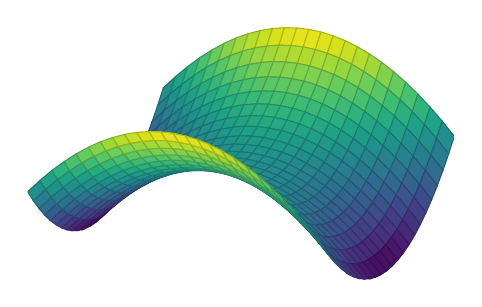
\begin{tikzpicture}
        \begin{axis}[    
            axis lines = none,       % 设置坐标轴通过原点
            xlabel = {$x$},            % x轴标签
            ylabel = {$y$},            % y轴标签
            zlabel = {$z$},            % z轴标签
            % title = {$z = y^2-x^2$},  % 图像标题
            % title style={at={(0.5,-0.1)}, anchor=north},
            colormap/viridis,          % 选择颜色映射
            ]
            \addplot3[
                surf,                    % 使用表面绘图
                domain=-3:3,              % x和y的范围
                y domain=-3:3,
            ]
            {y^2-x^2};    % 目标函数 z = sin(x^2 + y^2)
        \end{axis}
    \end{tikzpicture}
\end{center}
\begin{definition}
    For  $ p\in S $ in a surface,
    
    Call it  \name{elliptic} if  $ \det \dd N_p>0 $.
    
    Call it \name{hyperbolic} if  $ \det \dd N_p<0 $. 
    
    Call it \name{parabolic} if  $ \det \dd N_p=0 $ but  $ \dd N_p\neq 0 $, or call it \name{planar} if  $ \dd N_p=0 $.   
\end{definition}

The 1st fundamental form $ \Romannumer1_p=E\dd u^2+2F\dd u\dd v+G\dd v^2 $ where 
\begin{equation}
    E=\<X_u,X_u\>,\,F=\<X_u,X_v\>,\,G=\<X_v,X_v\>
\end{equation} 

However,
$ \Romannumer2(\alpha')=e\dd u^2+2f\dd u\dd v+g\dd v^2 $ where
\begin{equation}
    e=\<N,X_{u,u}\>,\, f=\<N,X_{u,v}\>,\, g=\<N,X_{v,v}\>
\end{equation} 

Since  $ \{X_u,X_v, N\} $ is an orthogonormal basis in  $ \Rbb^3 $,  $ \<N,N\>=1 $  $ \Rightarrow  $  $ 2\<N_u,N\>=0 $ if we take  $ \dps\frac{\partial }{\partial u} $. Then 
\[\begin{cases}
    N_u=a_{11}X_u+a_{21}X_v\\
    N_v=a_{12}X_u+a_{22}X_v
\end{cases}\]  
Then for  $ \dd N(\alpha')=\dd N(X_u\cdot u'+X_v\cdot v')=\begin{pmatrix}
    a_{11}&a_{12}\\
    a_{21}&a_{22}
\end{pmatrix}\cdot\begin{pmatrix}
    u'\\
    v'
\end{pmatrix}$. Therefore,  $ \dd N=\begin{pmatrix}
    a_{11}&a_{12}\\
    a_{21}&a_{22}
\end{pmatrix} $. Now 
\[f=\<N,X_{u,v}\>=-\<N_v,X_u\>=-\<a_{12}X_u+a_{22}X_v,X_u\>=-a_{12}E-a_{22}F\]
Similarly, one can prove 
\[f=-\<N_v,X_u\>=-a_{12}E-a_{22}F\]
\[e=-\<N_u,X_u\>=-a_{11}E-a_{21}F\]
\[g=-\<N_v,X_v\>=-a_{12}F-a_{22}G\]

So 
\[-\begin{pmatrix}
    e&f\\
    f&g 
\end{pmatrix}=\begin{pmatrix}
    a_{11}&a_{12}\\
    a_{21}&a_{22}   
\end{pmatrix}\begin{pmatrix}
    E&F\\
    F&G
\end{pmatrix}\]
 $ \Rightarrow  $ 
\begin{equation}
    \begin{pmatrix}
        a_{11}&a_{12}\\
        a_{21}&a_{22}
    \end{pmatrix}=-\frac{1}{EG-F^2}\begin{pmatrix}
        e&f\\
        f&g
    \end{pmatrix}\begin{pmatrix}
        G&-F\\
        -F&E
    \end{pmatrix}
\end{equation} 
\ie 
\begin{equation}
    \begin{aligned}
        &a_{11}=\frac{fF-eG}{EG-F^2}&a_{12}=\frac{gF-fG}{EG-F^2}\\
        &a_{21}=\frac{eF-fE}{EG-F^2}&a_{22}=\frac{fE-gE}{EG-F^2}
    \end{aligned}
\end{equation}
So  $ K=\det \dd N_p=\dps\frac{eg-f^2}{EG-F^2} $,  $ H=-\tr \dd N_p=\dps\frac{1}{2}\cdot\frac{eG-2fF+gE}{EG-F^2}$. 

\begin{example}
    For torus  $ T^2=S^1\times S^1 $, 
    
    $ X(u,v)=((a+r\cos u)\cos v,(a+r\cos u)\sin v,r\sin u) $.

    Then we can calculate  $ E,F,G,N $ by calculating  $ X_u,X_v $. And we obtain  $ f,g,e $ in a similar way. The result 
    \[K=\frac{eg-f^2}{EG-F^2}=\frac{\cos u}{r(a+r\cos v)}\]  
    Then 
    \[\begin{cases}
        K=0&u=\dps\frac{\pi}{2}\text{ or }\frac{3\pi}{2}\\
        K<0&\dps\frac{3\pi}{2}>u>\frac{\pi}{2}\\
        K>0&\text{otherwise}
    \end{cases}\] 

    So the torus is elliptic in the outer half and is hyperbolic in the inner half. 

    \begin{center}     
        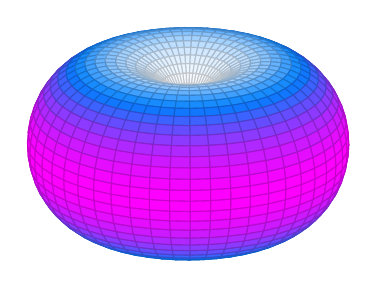
\begin{tikzpicture}
            \begin{axis}[
                axis lines = none,
            ]
                \addplot3[surf,
                colormap/cool,
                samples=50,
                domain=0:2*pi,y domain=0:2*pi,
                z buffer=sort,
                point meta={x * x + y * y}
                ]
               ({(2 + 2 * cos(deg(x))) * cos(deg(y + pi/2))}, 
                {(2 + 2 * cos(deg(x))) * sin(deg(y + pi/2))}, 
                {2 * sin(deg(x))});
            \end{axis}
        \end{tikzpicture}
    \end{center}
    
\end{example}

\begin{theorem}[Gauss Theorem Egregium]\label{Gauss fantanstic theorem}
    $ K  $ is the invariant of  $ S $, only depending on  $ E,F,G $.  Equivalently, Gauss curvature is invariant under local isometry.
\end{theorem}
\begin{proof}
    For  $ \{X_u,X_v,N\} $ an orthogonormal basis of  $ \Rbb^3 $, let 
    \[X_{u,u}=\Gamma^1_{11}X_u+\Gamma_{11}^2X_v+L_1N\]
    \[X_{u,v}=\Gamma_{12}^1X_u+\Gamma_{12}^2X_v+L_2N\]  
    \[X_{v,u}=\Gamma_{21}^1X_u+\Gamma_{21}^2X_v+\tilde{L}_2N\]
    \[X_{v,v}=\Gamma_{22}^1X_u+\Gamma_{22}^2X_v+L_3N\]
    where  $ \Gamma_{ij}^k $ is called \name{Cristopher symbol},  $ \Gamma_{21}^i=\Gamma_{21}^i,i=1,2 $ 
    \[N_u=a_{11}X_u+a_{12}X_v\]
    \[N_v=a_{12}X_u+a_{22}X_v\]
    Then take the inner product of  $ X_{u,u} $ with  $ N,X_u,X_v $ separately  
    \[e=\<X_{u,u},N\>=L_1\]
    \[\frac{1}{2}E_u=\frac{1}{2}\cdot\frac{\partial }{\partial u}\<X_u,X_u\>=\<X_{u,u},X_u\>=\Gamma_{1,1}^1E+\Gamma_{12}^2F\]
    \[F_u-\frac{1}{2}E_v=\<X_{u,u},X_v\>=\Gamma_{11}^1F+\Gamma_{11}^2G\]
    So we have  $ \begin{cases}
        L_1=e\\
        \Gamma_{11}^1E+\Gamma_{11}^2F=\dps\frac{1}{2}E_u\\
        \Gamma_{11}^1F+\Gamma_{11}^2G=\dps\frac{1}{2}F_u-\frac{1}{2}E_v
    \end{cases} $ \ie 
    \begin{equation}
        \begin{pmatrix}
            \Gamma_{11}^1\\
            \Gamma_{11}^2
        \end{pmatrix}=\begin{pmatrix}
            E&F\\
            F&G
        \end{pmatrix}^{-1}\begin{pmatrix}
            \dps\frac{1}{2}E_u\\
            F_u-\frac{1}{2}E_v
        \end{pmatrix}
    \end{equation}
    So any  $ \Gamma_{ij}^k $ can be represented by  $ E,F,G $.
    
    Now since   $ (X_{u,u})_v=(X_{v,v})_u $.
    
    \begin{equation}
        \begin{aligned}
            \frac{\partial }{\partial v}X_{u,u}&=((\Gamma_{11}^1)_vX_u+\Gamma_{11}^1X_{uv})+((\Gamma_{11}^2)_vX_v+\Gamma_{11}^2X_{vv})+((e_1)_vN+eN_v)\\
            &=(\Gamma_{11}^1)_vX_u+\Gamma_{11}^1((\Gamma_{12}^1)X_u+\Gamma_{12}^2X_v+fN)\\
            &+(\Gamma_{11}^2)_vX_v+\Gamma_{11}^2(\Gamma_{22}^1X_u+\Gamma_{22}^2X_v+gN)\\
            &+e_vN+e(a_{12}X_u+a_{22}X_v)
        \end{aligned}
    \end{equation}
    Similarly, one can calculate that
    \begin{equation}
        \begin{aligned}
            \frac{\partial}{\partial u}X_{u,v}&=(\Gamma_{12}^1)_uX_u+\Gamma_{12}^1(\Gamma_{11}^1X_u+\Gamma_{11}^2X_v+eN)\\
            &+(\Gamma_{12}^2)_uX_v+\Gamma_{12}^2(\Gamma_{12}^1X_u+\Gamma_{12}^2X_v+fN)\\
            &+f_uN+f(a_{11}X_u+a_{21}X_v)
        \end{aligned}
    \end{equation}
    The coefficients of  $ X_v $ is 
    \[\Gamma_{11}^1\Gamma_{12}^2+(\Gamma_{11}^2)_v+\Gamma_{11}^2\Gamma_{22}^2+ea_{22}=\Gamma_{12}^1\Gamma_{11}^2+(\Gamma_{12}^2)_u+\Gamma_{12}^2\Gamma_{12}^2+fa_{21}\]
    where 
    \[ea_{22}-fa_{21}=\frac{(efF-egE)-(feF-f^2E)}{EG-F^2}=\frac{(f^2-eg)E}{EG-F^2}=-KE\]
    So we obtain
    \begin{equation}
        \frac{(\Gamma_{11}^1\Gamma_{12}^2+(\Gamma_{11}^2)_v+\Gamma_{11}^2\Gamma_{22}^2)-(\Gamma_{12}^1\Gamma_{11}^2+(\Gamma_{12}^2)_u+\Gamma_{12}^2\Gamma_{12}^2)}{E}=K
    \end{equation} 

    Here we have proved that  $ K  $ can be represented by  $ E,F,G $.
\end{proof}

This is the \name{Gauss formula} we obtain 
\begin{equation}\label{Gauss equation 1}
    (\Gamma_{12}^2)_u-(\Gamma_{11}^2)_v+\Gamma_{12}^1\Gamma_{11}^2+\Gamma_{12}^2\Gamma_{12}^2-\Gamma_{11}^2\Gamma_{22}^2-\Gamma_{11}^1\Gamma_{12}^2=-EK
\end{equation}

Similarly, one can prove for the coefficients of  $ X_u $
    \begin{equation}\label{Gauss equation 2}
        (\Gamma_{12}^1)_u-(\Gamma_{11}^1)_v+\Gamma_{12}^2\Gamma_{12}^1-\Gamma_{11}^2\Gamma_{22}^1=FK
    \end{equation}
It is (when  $ F\neq 0 $) merely another form of the Gauss formula.

    And the coefficients of  $ N $
    \begin{equation}\label{Gauss equation 3}
        e_v-f_u=e\Gamma_{12}^1-f(\Gamma_{12}^2-\Gamma_{11}^1)-g\Gamma_{11}^2
    \end{equation} 

By applying the same process  to  $ (x_{v,v})_u=(x_{u,v})_v $, we obtain the equation giving again the
Gauss formula \eqref{Gauss equation 1}. Furthermore, we can obtain another equation 

\begin{equation}\label{Gauss equation 4}
    f_v-g_u=e\Gamma_{22}^1+f(\Gamma_{22}^2-\Gamma_{12}^1)-g\Gamma_{12}^2        
\end{equation}
\eqref{Gauss equation 3} and \eqref{Gauss equation 4} are called \name{Maindardi-Codazzi} equations

The Gauss formula and the Mainardi-Codazzi equations are known under the name of compatibility equations of the theory of surfaces.
\begin{theorem}
    If  $ E,F,G,e,f,g $ satisfies \eqref{Gauss equation 1}  $ \sim $  \eqref{Gauss equation 4}, then it uniquely determines a surface.
\end{theorem}
% \tikzset{external/export=true}

% \begin{tikzcd}[arrow style=math font,cells={nodes={text height=2ex,text depth=0.75ex}}]
% 	\cdots & H_{k-1}(U) \oplus H_{k-1}(V) \arrow[l] \arrow[draw=none]{d}[name=Y, shape=coordinate]{} & \arrow[l] H_{k-1}(U \cap V) \\
% 	H_{k}(M) \arrow[curarrow=Y]{urr}{} & H_{k}(U) \oplus H_{k}(V) \arrow[l] \arrow[draw=none]{d}[name=Z,shape=coordinate]{} & H_{k}(U \cap V) \arrow[l] \\
% 	H_{k+1}(M) \arrow[curarrow=Z]{urr}{} & H_{k+1}(U) \oplus H_{k+1}(V) \arrow[l] & \cdots \arrow[l]
% \end{tikzcd}



% \begin{tikzpicture}
% 	\begin{axis}[view={0}{90},domain=-4:4,axis lines=middle,xlabel={$ x $},ylabel={$ y $}]
% 	\addplot3 [blue,-stealth,samples=16,
% 			quiver={
% 				u={-y},
% 				v={x},
% 				scale arrows=0.2,
% 			},
% 		] { 1}; % use pow(x^2 + y^2,1/2) if you choose to have a real 3D plot
% 	\end{axis}
% 	\end{tikzpicture}
\printindex
\newpage
\listoftheorems[ignoreall, show={theorem,proposition}]
\end{document}

%%%%%%%%%%%
% 
% \documentclass[x11names, border=5pt]{standalone}

% \usepackage{pst-plot}
% \usepackage{auto-pst-pdf}

% \begin{document}
% %
% %%%%%%%%%%% v(x, y) = =x² + y² - 1
% \psset{unit=4cm, arrowinset=0.12}
% \begin{pspicture}(-1.2,-1.2)(1.1,1.1)
%     \psaxes[ticksize=0 4pt,axesstyle=frame,tickstyle=inner,subticks=20,
%     Ox=-1,Oy=-1](-1,-1)(1,1)
%     \psset{arrows=->,algebraic}
%     \psVectorfield[linecolor=DarkOliveGreen3](-0.9,-0.9)(0.9,0.9){ x²+y²-1 }
% \end{pspicture}

% \end{document} 


%%%%%%%%


%%%%%%%%
% An example to draw Mayer-Vietoris sequence 
% \documentclass{article}
% \usepackage{tikz-cd}



% \begin{document}

%     \begin{tikzcd}[arrow style=math font,cells={nodes={text height=2ex,text depth=0.75ex}}]
%        \cdots & H_{k-1}(U) \oplus H_{k-1}(V) \arrow[l] \arrow[draw=none]{d}[name=Y, shape=coordinate]{} & \arrow[l] H_{k-1}(U \cap V) \\
%        H_{k}(M) \arrow[curarrow=Y]{urr}{} & H_{k}(U) \oplus H_{k}(V) \arrow[l] \arrow[draw=none]{d}[name=Z,shape=coordinate]{} & H_{k}(U \cap V) \arrow[l] \\
%        H_{k+1}(M) \arrow[curarrow=Z]{urr}{} & H_{k+1}(U) \oplus H_{k+1}(V) \arrow[l] & \cdots \arrow[l]
%    \end{tikzcd}

% \end{document}









%%%%%%%%